\pdfoutput=1
\pdfinclusioncopyfonts=1
%% Author: PGL  Porta Mana
%% Created: 2015-05-01T20:53:34+0200
%% Last-Updated: 2025-08-25T10:10:54+0200
%%%%%%%%%%%%%%%%%%%%%%%%%%%%%%%%%%%%%%%%%%%%%%%%%%%%%%%%%%%%%%%%%%%%%%%%%%%%
\newif\ifanon
\anontrue
\newif\ifarxiv
\arxivfalse
%\iftrue\pdfmapfile{+classico.map}\fi
\newif\ifafour
\afourtrue% true = A4, false = A5
% \newif\iftypodisclaim % typographical disclaim on the side
% \typodisclaimfalse
\newcommand*{\memfontfamily}{zpl}
%\newcommand*{\memfontenc}{T1}
\newcommand*{\memfontpack}{newpx}
\documentclass[a4paper,12pt,%extrafontsizes,%
onecolumn,oneside,%titlepage,%french,italian,german,swedish,latin,
british%
]{memoir}
\newcommand*{\firstdraft}{15 January 2025}
\newcommand*{\version}{0.1}
\newcommand*{\updated}{\ifarxiv***\else\today\enskip\DTMsetstyle{iso}\DTMcurrenttime\fi}
\newcommand*{\propertitle}{The Seven Wonders of the World%\\[\jot]\Large Notes on 21st-century physics
\\[3\jot]\LARGE\itshape Exercises}
%\newcommand*{\propertitle}{The Seven Wonders of the World\\[\jot]\Large Lecture notes for ING\,175}
\newcommand*{\pdftitle}{The Seven Wonders of the World: Exercises}
\newcommand*{\pdfauthor}{P.G.L.  Porta Mana}
% \newcommand*{\headauthor}{\nameref}
\newcommand*{\reporthead}{\iftrue\else Open Science Framework \href{https://doi.org/10.31219/osf.io/***}{\textsc{doi}:10.31219/osf.io/***}\fi}% Report number

%%%%%%%%%%%%%%%%%%%%%%%%%%%%%%%%%%%%%%%%%%%%%%%%%%%%%%%%%%%%%%%%%%%%%%%%%%%%
%%% Calls to packages (uncomment as needed)
%%%%%%%%%%%%%%%%%%%%%%%%%%%%%%%%%%%%%%%%%%%%%%%%%%%%%%%%%%%%%%%%%%%%%%%%%%%%

%\usepackage{pifont}

%\usepackage{fontawesome}
\PassOptionsToPackage{obeyspaces}{url}
\usepackage[T1]{fontenc}
\input{glyphtounicode} \pdfgentounicode=1

\usepackage[utf8]{inputenx}

%\usepackage{newunicodechar}
% \newunicodechar{Ĕ}{\u{E}}
% \newunicodechar{ĕ}{\u{e}}
% \newunicodechar{Ĭ}{\u{I}}
% \newunicodechar{ĭ}{\u{\i}}
% \newunicodechar{Ŏ}{\u{O}}
% \newunicodechar{ŏ}{\u{o}}
% \newunicodechar{Ŭ}{\u{U}}
% \newunicodechar{ŭ}{\u{u}}
% \newunicodechar{Ā}{\=A}
% \newunicodechar{ā}{\=a}
% \newunicodechar{Ē}{\=E}
% \newunicodechar{ē}{\=e}
% \newunicodechar{Ī}{\=I}
% \newunicodechar{ī}{\={\i}}
% \newunicodechar{Ō}{\=O}
% \newunicodechar{ō}{\=o}
% \newunicodechar{Ū}{\=U}
% \newunicodechar{ū}{\=u}
% \newunicodechar{Ȳ}{\=Y}
% \newunicodechar{ȳ}{\=y}

\newcommand*{\bmmax}{3} % reduce number of bold fonts, before font packages
\newcommand*{\hmmax}{0} % reduce number of heavy fonts, before font packages

\usepackage{textcomp}

%\usepackage[normalem]{ulem}% package for underlining
% \makeatletter
% \def\ssout{\bgroup \ULdepth=-.35ex%\UL@setULdepth
%  \markoverwith{\lower\ULdepth\hbox
%    {\kern-.03em\vbox{\hrule width.2em\kern1.2\p@\hrule}\kern-.03em}}%
%  \ULon}
% \makeatother

\usepackage{amsmath}

\usepackage{mathtools}
%\addtolength{\jot}{\jot} % increase spacing in multiline formulae
\setlength{\multlinegap}{0pt}

%\usepackage{empheq}% automatically calls amsmath and mathtools
%\newcommand*{\widefbox}[1]{\fbox{\hspace{1em}#1\hspace{1em}}}

%%%% empheq above seems more versatile than these:
%\usepackage{fancybox}
%\usepackage{framed}

% \usepackage[misc]{ifsym} % for dice
% \newcommand*{\diceone}{{\scriptsize\Cube{1}}}

\usepackage{amssymb}

\usepackage{amsxtra}

\usepackage[main=british]{babel}\selectlanguage{british}
%\newcommand*{\langnohyph}{\foreignlanguage{nohyphenation}}
\newcommand{\langnohyph}[1]{\begin{hyphenrules}{nohyphenation}#1\end{hyphenrules}}

\usepackage[autostyle=false,autopunct=false,english=british]{csquotes}
\setquotestyle{american}
\newcommand*{\defquote}[1]{`\,#1\,'}

% \makeatletter
% \renewenvironment{quotation}%
%                {\list{}{\listparindent 1.5em%
%                         \itemindent    \listparindent
%                         \rightmargin=1em   \leftmargin=1em
%                         \parsep        \z@ \@plus\p@}%
%                 \item[]\footnotesize}%
%                 {\endlist}
% \makeatother


% \usepackage{amsthm}
% %% from https://tex.stackexchange.com/a/404680/97039
% \makeatletter
% \def\@endtheorem{\endtrivlist}
% \makeatother

% \newcommand*{\QED}{\textsc{q.e.d.}}
% \renewcommand*{\qedsymbol}{\QED}
% \theoremstyle{remark}
% \newtheorem{note}{Note}
% \newtheorem*{remark}{Note}
% \newtheoremstyle{innote}{\parsep}{\parsep}{\footnotesize}{}{}{}{0pt}{}
% \theoremstyle{innote}
% \newtheorem*{innote}{}

\usepackage[shortlabels,inline]{enumitem}
\SetEnumitemKey{para}{itemindent=\parindent,leftmargin=0pt,listparindent=\parindent,parsep=0pt,itemsep=\topsep}
% \SetEnumitemKey{shift}{leftmargin=8.81pt}
\SetEnumitemKey{exerc}{leftmargin=17.62pt,label=\bfseries\arabic*.}
% \begin{asparaenum} = \begin{enumerate}[para]
% \begin{inparaenum} = \begin{enumerate*}
\setlist{itemsep=0pt,topsep=\parsep}
\setlist[enumerate,2]{label=(\roman*)}
\setlist[enumerate]{label=(\alph*),leftmargin=26.44pt}
\setlist[itemize]{leftmargin=26.44pt}% parindent is 17.62482pt
\setlist[description]{leftmargin=26.44pt,font=\sffamily\bfseries}
% old alternative:
% \setlist[enumerate,2]{label=\alph*.}
% \setlist[enumerate]{leftmargin=\parindent}
% \setlist[itemize]{leftmargin=\parindent}
% \setlist[description]{leftmargin=\parindent}

\usepackage[babel,theoremfont,largesc,smallerops,nosymbolsc]{newpx}

% For Baskerville see https://ctan.org/tex-archive/fonts/baskervillef?lang=en
% and http://mirrors.ctan.org/fonts/baskervillef/doc/baskervillef-doc.pdf
% \usepackage[p]{baskervillef}
% \usepackage[varqu,varl,var0]{inconsolata}
% \usepackage[scale=.95,type1]{cabin}
% \usepackage[baskerville,vvarbb]{newtxmath}
% \usepackage[cal=boondoxo]{mathalfa}


% \usepackage[bigdelims,nosymbolsc%,smallerops % probably arXiv doesn't have it
% ]{newpxmath}
%\useosf
%\linespread{1.083}%
%\linespread{1.05}% widely used
\linespread{1.1}% best for text with maths
%% smaller operators for old version of newpxmath
\makeatletter
\def\re@DeclareMathSymbol#1#2#3#4{%
    \let#1=\undefined
    \DeclareMathSymbol{#1}{#2}{#3}{#4}}
%\re@DeclareMathSymbol{\bigsqcupop}{\mathop}{largesymbols}{"46}
%\re@DeclareMathSymbol{\bigodotop}{\mathop}{largesymbols}{"4A}
\re@DeclareMathSymbol{\bigoplusop}{\mathop}{largesymbols}{"4C}
\re@DeclareMathSymbol{\bigotimesop}{\mathop}{largesymbols}{"4E}
\re@DeclareMathSymbol{\sumop}{\mathop}{largesymbols}{"50}
\re@DeclareMathSymbol{\prodop}{\mathop}{largesymbols}{"51}
\re@DeclareMathSymbol{\bigcupop}{\mathop}{largesymbols}{"53}
\re@DeclareMathSymbol{\bigcapop}{\mathop}{largesymbols}{"54}
%\re@DeclareMathSymbol{\biguplusop}{\mathop}{largesymbols}{"55}
\re@DeclareMathSymbol{\bigwedgeop}{\mathop}{largesymbols}{"56}
\re@DeclareMathSymbol{\bigveeop}{\mathop}{largesymbols}{"57}
%\re@DeclareMathSymbol{\bigcupdotop}{\mathop}{largesymbols}{"DF}
%\re@DeclareMathSymbol{\bigcapplusop}{\mathop}{largesymbolsPXA}{"00}
%\re@DeclareMathSymbol{\bigsqcupplusop}{\mathop}{largesymbolsPXA}{"02}
%\re@DeclareMathSymbol{\bigsqcapplusop}{\mathop}{largesymbolsPXA}{"04}
%\re@DeclareMathSymbol{\bigsqcapop}{\mathop}{largesymbolsPXA}{"06}
\re@DeclareMathSymbol{\bigtimesop}{\mathop}{largesymbolsPXA}{"10}
%\re@DeclareMathSymbol{\coprodop}{\mathop}{largesymbols}{"60}
%\re@DeclareMathSymbol{\varprod}{\mathop}{largesymbolsPXA}{16}
\makeatother
%%
%% With euler font cursive for Greek letters - the [1] means 100% scaling
\DeclareFontFamily{U}{egreek}{\skewchar\font'177}%
\DeclareFontShape{U}{egreek}{m}{n}{<-6>s*[1]eurm5 <6-8>s*[1]eurm7 <8->s*[1]eurm10}{}%
\DeclareFontShape{U}{egreek}{m}{it}{<->s*[1]eurmo10}{}%
\DeclareFontShape{U}{egreek}{b}{n}{<-6>s*[1]eurb5 <6-8>s*[1]eurb7 <8->s*[1]eurb10}{}%
\DeclareFontShape{U}{egreek}{b}{it}{<->s*[1]eurbo10}{}%
\DeclareSymbolFont{egreeki}{U}{egreek}{m}{it}%
\SetSymbolFont{egreeki}{bold}{U}{egreek}{b}{it}% from the amsfonts package
\DeclareSymbolFont{egreekr}{U}{egreek}{m}{n}%
\SetSymbolFont{egreekr}{bold}{U}{egreek}{b}{n}% from the amsfonts package
% Take also \sum, \prod, \coprod symbols from Euler fonts
\DeclareFontFamily{U}{egreekx}{\skewchar\font'177}
\DeclareFontShape{U}{egreekx}{m}{n}{%
       <-7.5>s*[0.9]euex7%
    <7.5-8.5>s*[0.9]euex8%
    <8.5-9.5>s*[0.9]euex9%
    <9.5->s*[0.9]euex10%
}{}
\DeclareSymbolFont{egreekx}{U}{egreekx}{m}{n}
\DeclareMathSymbol{\sumop}{\mathop}{egreekx}{"50}
\DeclareMathSymbol{\prodop}{\mathop}{egreekx}{"51}
\DeclareMathSymbol{\coprodop}{\mathop}{egreekx}{"60}
\makeatletter
\def\sum{\DOTSI\sumop\slimits@}
\def\prod{\DOTSI\prodop\slimits@}
\def\coprod{\DOTSI\coprodop\slimits@}
\makeatother
%%%% Greek letters not usually given in LaTeX
%%%% best to uncomment only the ones needed
%% %% \input{definegreek.tex} % originally in a separate file
% \DeclareMathSymbol{\varpartial}{\mathalpha}{egreeki}{"40}
% \DeclareMathSymbol{\partialup}{\mathalpha}{egreekr}{"40}
% \DeclareMathSymbol{\alpha}{\mathalpha}{egreeki}{"0B}
% \DeclareMathSymbol{\beta}{\mathalpha}{egreeki}{"0C}
% \DeclareMathSymbol{\gamma}{\mathalpha}{egreeki}{"0D}
% \DeclareMathSymbol{\delta}{\mathalpha}{egreeki}{"0E}
% \DeclareMathSymbol{\epsilon}{\mathalpha}{egreeki}{"0F}
% \DeclareMathSymbol{\zeta}{\mathalpha}{egreeki}{"10}
% \DeclareMathSymbol{\eta}{\mathalpha}{egreeki}{"11}
% \DeclareMathSymbol{\theta}{\mathalpha}{egreeki}{"12}
% \DeclareMathSymbol{\iota}{\mathalpha}{egreeki}{"13}
% \DeclareMathSymbol{\kappa}{\mathalpha}{egreeki}{"14}
% \DeclareMathSymbol{\lambda}{\mathalpha}{egreeki}{"15}
% \DeclareMathSymbol{\mu}{\mathalpha}{egreeki}{"16}
% \DeclareMathSymbol{\nu}{\mathalpha}{egreeki}{"17}
% \DeclareMathSymbol{\xi}{\mathalpha}{egreeki}{"18}
% \DeclareMathSymbol{\omicron}{\mathalpha}{egreeki}{"6F}
% \DeclareMathSymbol{\pi}{\mathalpha}{egreeki}{"19}
% \DeclareMathSymbol{\rho}{\mathalpha}{egreeki}{"1A}
% \DeclareMathSymbol{\sigma}{\mathalpha}{egreeki}{"1B}
% \DeclareMathSymbol{\tau}{\mathalpha}{egreeki}{"1C}
% \DeclareMathSymbol{\upsilon}{\mathalpha}{egreeki}{"1D}
% \DeclareMathSymbol{\phi}{\mathalpha}{egreeki}{"1E}
% \DeclareMathSymbol{\chi}{\mathalpha}{egreeki}{"1F}
% \DeclareMathSymbol{\psi}{\mathalpha}{egreeki}{"20}
% \DeclareMathSymbol{\omega}{\mathalpha}{egreeki}{"21}
% \DeclareMathSymbol{\varepsilon}{\mathalpha}{egreeki}{"22}
% \DeclareMathSymbol{\vartheta}{\mathalpha}{egreeki}{"23}
% \DeclareMathSymbol{\varpi}{\mathalpha}{egreeki}{"24}
% \let\varrho\rho
% \let\varsigma\sigma
% \let\varkappa\kappa
% \DeclareMathSymbol{\varphi}{\mathalpha}{egreeki}{"27}
% %
% \DeclareMathSymbol{\varAlpha}{\mathalpha}{egreeki}{"41}
% \DeclareMathSymbol{\varBeta}{\mathalpha}{egreeki}{"42}
% \DeclareMathSymbol{\varGamma}{\mathalpha}{egreeki}{"00}
% \DeclareMathSymbol{\varDelta}{\mathalpha}{egreeki}{"01}
% \DeclareMathSymbol{\varEpsilon}{\mathalpha}{egreeki}{"45}
% \DeclareMathSymbol{\varZeta}{\mathalpha}{egreeki}{"5A}
% \DeclareMathSymbol{\varEta}{\mathalpha}{egreeki}{"48}
% \DeclareMathSymbol{\varTheta}{\mathalpha}{egreeki}{"02}
% \DeclareMathSymbol{\varIota}{\mathalpha}{egreeki}{"49}
% \DeclareMathSymbol{\varKappa}{\mathalpha}{egreeki}{"4B}
% \DeclareMathSymbol{\varLambda}{\mathalpha}{egreeki}{"03}
% \DeclareMathSymbol{\varMu}{\mathalpha}{egreeki}{"4D}
% \DeclareMathSymbol{\varNu}{\mathalpha}{egreeki}{"4E}
% \DeclareMathSymbol{\varXi}{\mathalpha}{egreeki}{"04}
% \DeclareMathSymbol{\varOmicron}{\mathalpha}{egreeki}{"4F}
% \DeclareMathSymbol{\varPi}{\mathalpha}{egreeki}{"05}
% \DeclareMathSymbol{\varRho}{\mathalpha}{egreeki}{"50}
% \DeclareMathSymbol{\varSigma}{\mathalpha}{egreeki}{"06}
% \DeclareMathSymbol{\varTau}{\mathalpha}{egreeki}{"54}
% \DeclareMathSymbol{\varUpsilon}{\mathalpha}{egreeki}{"07}
% \DeclareMathSymbol{\varPhi}{\mathalpha}{egreeki}{"08}
% \DeclareMathSymbol{\varChi}{\mathalpha}{egreeki}{"58}
% \DeclareMathSymbol{\varPsi}{\mathalpha}{egreeki}{"09}
% \DeclareMathSymbol{\varOmega}{\mathalpha}{egreeki}{"0A}
% %
% \DeclareMathSymbol{\Alpha}{\mathalpha}{egreekr}{"41}
% \DeclareMathSymbol{\Beta}{\mathalpha}{egreekr}{"42}
% \DeclareMathSymbol{\Gamma}{\mathalpha}{egreekr}{"00}
% \DeclareMathSymbol{\Delta}{\mathalpha}{egreekr}{"01}
% \DeclareMathSymbol{\Epsilon}{\mathalpha}{egreekr}{"45}
% \DeclareMathSymbol{\Zeta}{\mathalpha}{egreekr}{"5A}
% \DeclareMathSymbol{\Eta}{\mathalpha}{egreekr}{"48}
% \DeclareMathSymbol{\Theta}{\mathalpha}{egreekr}{"02}
% \DeclareMathSymbol{\Iota}{\mathalpha}{egreekr}{"49}
% \DeclareMathSymbol{\Kappa}{\mathalpha}{egreekr}{"4B}
% \DeclareMathSymbol{\Lambda}{\mathalpha}{egreekr}{"03}
% \DeclareMathSymbol{\Mu}{\mathalpha}{egreekr}{"4D}
% \DeclareMathSymbol{\Nu}{\mathalpha}{egreekr}{"4E}
% \DeclareMathSymbol{\Xi}{\mathalpha}{egreekr}{"04}
% \DeclareMathSymbol{\Omicron}{\mathalpha}{egreekr}{"4F}
% \DeclareMathSymbol{\Pi}{\mathalpha}{egreekr}{"05}
% \DeclareMathSymbol{\Rho}{\mathalpha}{egreekr}{"50}
% \DeclareMathSymbol{\Sigma}{\mathalpha}{egreekr}{"06}
% \DeclareMathSymbol{\Tau}{\mathalpha}{egreekr}{"54}
% \DeclareMathSymbol{\Upsilon}{\mathalpha}{egreekr}{"07}
% \DeclareMathSymbol{\Phi}{\mathalpha}{egreekr}{"08}
% \DeclareMathSymbol{\Chi}{\mathalpha}{egreekr}{"58}
% \DeclareMathSymbol{\Psi}{\mathalpha}{egreekr}{"09}
% \DeclareMathSymbol{\Omega}{\mathalpha}{egreekr}{"0A}
% %
% \DeclareMathSymbol{\alphaup}{\mathalpha}{egreekr}{"0B}
% \DeclareMathSymbol{\betaup}{\mathalpha}{egreekr}{"0C}
% \DeclareMathSymbol{\gammaup}{\mathalpha}{egreekr}{"0D}
% \DeclareMathSymbol{\deltaup}{\mathalpha}{egreekr}{"0E}
% \DeclareMathSymbol{\epsilonup}{\mathalpha}{egreekr}{"0F}
% \DeclareMathSymbol{\zetaup}{\mathalpha}{egreekr}{"10}
% \DeclareMathSymbol{\etaup}{\mathalpha}{egreekr}{"11}
% \DeclareMathSymbol{\thetaup}{\mathalpha}{egreekr}{"12}
% \DeclareMathSymbol{\iotaup}{\mathalpha}{egreekr}{"13}
% \DeclareMathSymbol{\kappaup}{\mathalpha}{egreekr}{"14}
% \DeclareMathSymbol{\lambdaup}{\mathalpha}{egreekr}{"15}
% \DeclareMathSymbol{\muup}{\mathalpha}{egreekr}{"16}
% \DeclareMathSymbol{\nuup}{\mathalpha}{egreekr}{"17}
% \DeclareMathSymbol{\xiup}{\mathalpha}{egreekr}{"18}
% \DeclareMathSymbol{\omicronup}{\mathalpha}{egreekr}{"6F}
% \DeclareMathSymbol{\piup}{\mathalpha}{egreekr}{"19}
% \DeclareMathSymbol{\rhoup}{\mathalpha}{egreekr}{"1A}
% \DeclareMathSymbol{\sigmaup}{\mathalpha}{egreekr}{"1B}
% \DeclareMathSymbol{\tauup}{\mathalpha}{egreekr}{"1C}
% \DeclareMathSymbol{\upsilonup}{\mathalpha}{egreekr}{"1D}
% \DeclareMathSymbol{\phiup}{\mathalpha}{egreekr}{"1E}
% \DeclareMathSymbol{\chiup}{\mathalpha}{egreekr}{"1F}
% \DeclareMathSymbol{\psiup}{\mathalpha}{egreekr}{"20}
% \DeclareMathSymbol{\omegaup}{\mathalpha}{egreekr}{"21}
% \DeclareMathSymbol{\varepsilonup}{\mathalpha}{egreekr}{"22}
% \DeclareMathSymbol{\varthetaup}{\mathalpha}{egreekr}{"23}
% \DeclareMathSymbol{\varpiup}{\mathalpha}{egreekr}{"24}
% \let\varrhoup\rhoup
% \let\varsigmaup\sigmaup
% \let\varkappaup\kappaup
% \DeclareMathSymbol{\varphiup}{\mathalpha}{egreekr}{"27}


\usepackage[scaled=0.837435]%
{DejaVuSansCondensed}%  sans-serif font
%\renewcommand\sfdefault{URWClassico-TLF}
\DeclareMathAlphabet{\mathsf}  {T1}{\sfdefault}{m}{sl}
\SetMathAlphabet{\mathsf}{bold}{T1}{\sfdefault}{b}{sl}
%\newcommand*{\mathte}[1]{\textbf{\textit{\textsf{#1}}}}
% Upright sans-serif math alphabet
% \DeclareMathAlphabet{\mathsu}  {T1}{\sfdefault}{m}{n}
% \SetMathAlphabet{\mathsu}{bold}{T1}{\sfdefault}{b}{n}

\usepackage[scaled=0.837435]%
{DejaVuSansMono}% typewriter text


\usepackage{mathdots}

\usepackage[usenames]{xcolor}
% Tol (2012) colour-blind-, print-, screen-friendly colours, alternative scheme; Munsell terminology
\definecolor{blue}{HTML}{4477AA}
\definecolor{cyan}{HTML}{66CCEE}
\definecolor{green}{HTML}{228833}
\definecolor{yellow}{HTML}{CCBB44}
\definecolor{red}{HTML}{EE6677}
\definecolor{purple}{HTML}{AA3377}
\definecolor{grey}{HTML}{BBBBBB}
\definecolor{midgrey}{HTML}{888888}
% \definecolor{darkgrey}{HTML}{555555}
\definecolor{darkgrey}{HTML}{333333}
\definecolor{lgrey}{HTML}{DDDDDD}
%\newcommand*\mycolourbox[1]{%
%\colorbox{grey}{\hspace{1em}#1\hspace{1em}}}
\colorlet{shadecolor}{lgrey}

\usepackage{bm}


\usepackage{microtype}

\usepackage[backend=biber,mcite,%subentry,
citestyle=authoryear-comp,bibstyle=pglpm_latex/pglpm-authoryear,autopunct=false,sorting=ny,sortcites=false,natbib=false,maxcitenames=2,maxbibnames=8,minbibnames=8,giveninits=true,uniquename=false,uniquelist=false,maxalphanames=1,block=space,hyperref=true,defernumbers=false,useprefix=true,sortupper=false,language=british,parentracker=false,autocite=inline,dashed=false]{biblatex}
\DeclareSortingTemplate{ny}{\sort{\field{sortname}\field{author}\field{editor}}\sort{\field{year}}}
\DeclareFieldFormat{postnote}{#1}
\iffalse\makeatletter%%% replace parenthesis with brackets
\newrobustcmd*{\parentexttrack}[1]{%
  \begingroup
  \blx@blxinit
  \blx@setsfcodes
  \blx@bibopenparen#1\blx@bibcloseparen
  \endgroup}
\AtEveryCite{%
  \let\parentext=\parentexttrack%
  \let\bibopenparen=\bibopenbracket%
  \let\bibcloseparen=\bibclosebracket}
\makeatother\fi
\DefineBibliographyExtras{british}{\def\finalandcomma{\addcomma}}
\renewcommand*{\finalnamedelim}{\addspace\amp\space}
% \renewcommand*{\finalnamedelim}{\addcomma\space}
\renewcommand*{\textcitedelim}{\addcomma\space}
% % These penalties are not needed with xurl loaded
% \setcounter{biburlucpenalty}{1}  %break URL after uppercase character
% \setcounter{biburlnumpenalty}{1} %break URL after number
% \setcounter{biburllcpenalty}{1}  %break URL after lowercase character
\DeclareDelimFormat{multicitedelim}{\addsemicolon\addspace\space}
\DeclareDelimFormat{compcitedelim}{\addsemicolon\addspace\space}
\DeclareDelimFormat{postnotedelim}{\addspace}
\ifarxiv\else\addbibresource{portamanabib.bib}\fi
\renewcommand{\nameyeardelim}{~}
\renewcommand{\bibfont}{\footnotesize}
%\appto{\citesetup}{\footnotesize}% smaller font for citations
\defbibheading{bibliography}[\bibname]{\chapter*{#1}\label{sec:biblio}\addcontentsline{toc}{chapter}{#1}%\markboth{#1}{#1}
}

\usepackage{xurl}
\PassOptionsToPackage{hyphens}{url}\usepackage[hypertexnames=false,pdfencoding=unicode,psdextra]{hyperref}
% % Not needed with xurl
% %\def\UrlOrds{\do\*\do\-\do\~\do\'\do\"\do\-}%
% % \def\myUrlOrds{\do\0\do\1\do\2\do\3\do\4\do\5\do\6\do\7\do\8\do\9\do\a\do\b\do\c\do\d\do\e\do\f\do\g\do\h\do\i\do\j\do\k\do\l\do\m\do\n\do\o\do\p\do\q\do\r\do\s\do\t\do\u\do\v\do\w\do\x\do\y\do\z\do\A\do\B\do\C\do\D\do\E\do\F\do\G\do\H\do\I\do\J\do\K\do\L\do\M\do\N\do\O\do\P\do\Q\do\R\do\S\do\T\do\U\do\V\do\W\do\X\do\Y\do\Z}%
% \makeatletter
% %\g@addto@macro\UrlSpecials{\do={\newline}}
% \g@addto@macro{\UrlBreaks}{%
% \do\0\do\1\do\2\do\3\do\4\do\5\do\6\do\7\do\8\do\9\do\a\do\b\do\c\do\d\do\e\do\f\do\g\do\h\do\i\do\j\do\k\do\l\do\m\do\n\do\o\do\p\do\q\do\r\do\s\do\t\do\u\do\v\do\w\do\x\do\y\do\z\do\A\do\B\do\C\do\D\do\E\do\F\do\G\do\H\do\I\do\J\do\K\do\L\do\M\do\N\do\O\do\P\do\Q\do\R\do\S\do\T\do\U\do\V\do\W\do\X\do\Y\do\Z%
% }
% % \g@addto@macro\UrlSpecials{%
% % \do\/{\mbox{\UrlFont/}\hskip 0pt plus 10pt}%
% % }
% \makeatother
\newcommand*{\citep}{\footcites}
\newcommand*{\citey}{\footcites}%{\parencites*}
\newcommand*{\ibid}{\unspace\addtocounter{footnote}{-1}\footnotemark{}}
%\renewcommand*{\cite}{\parencite}
%\renewcommand*{\cites}{\parencites}
\providecommand{\href}[2]{#2}
\providecommand{\eprint}[2]{\texttt{\href{#1}{#2}}}
\newcommand*{\amp}{\&}
% \newcommand*{\citein}[2][]{\textnormal{\textcite[#1]{#2}}%\addtocategory{extras}{#2}
% }
\newcommand*{\citein}[2][]{\textnormal{\textcite[#1]{#2}}%\addtocategory{extras}{#2}
}
\newcommand*{\citebi}[2][]{\textcite[#1]{#2}%\addtocategory{extras}{#2}
}
\newcommand*{\subtitleproc}[1]{}
\newcommand*{\chapb}{ch.}

\newcommand*{\arxiveprint}[1]{%
arXiv \doi{10.48550/arXiv.#1}%
}
\newcommand*{\mparceprint}[1]{%
\href{http://www.ma.utexas.edu/mp_arc-bin/mpa?yn=#1}{mp_arc:\allowbreak\nolinkurl{#1}}%
}
\newcommand*{\haleprint}[1]{%
\href{https://hal.archives-ouvertes.fr/#1}{\textsc{hal}:\allowbreak\nolinkurl{#1}}%
}
\newcommand*{\philscieprint}[1]{%
\href{http://philsci-archive.pitt.edu/archive/#1}{PhilSci:\allowbreak\nolinkurl{#1}}%
}
\newcommand*{\doi}[1]{%
\href{https://doi.org/#1}{\textsc{doi}:\allowbreak\nolinkurl{#1}}%
}
\newcommand*{\biorxiveprint}[1]{%
bioRxiv \doi{10.1101/#1}%
}
\newcommand*{\osfeprint}[1]{%
Open Science Framework \doi{10.31219/osf.io/#1}%
}
\newcommand*{\osfproj}[1]{%
Open Science Framework \doi{10.17605/osf.io/#1}%
}

\usepackage{graphicx}
\usepackage{graphbox}

%\usepackage{tikz-cd}

\usepackage{pdfrender}
\newcommand*{\textxbf}[1]{\textpdfrender{TextRenderingMode=2,LineWidth=0.2pt}{\textbf{#1}}}
\renewcommand*{\bm}[1]{\textpdfrender{TextRenderingMode=2,LineWidth=0.2pt}{\boldsymbol{#1}}}

\usepackage[depth=3]{bookmark}
\hypersetup{%
colorlinks=true,
%pdfborderstyle={/S/U/W 0.5},
bookmarksnumbered,pdfborder={0 0 0.25},
citebordercolor=blue,citecolor=blue,linkbordercolor=blue,linkcolor=blue,urlbordercolor=green,urlcolor=green,breaklinks=true,pdftitle={\pdftitle},pdfauthor={\pdfauthor}}
% \usepackage[vertfit=local]{breakurl}% only for arXiv
\providecommand*{\urlalt}{\href}
% \makeatletter
% \DeclareUrlCommand\ULurl@@{%
%   \def\UrlFont{\ttfamily\color{cyan}}%
%   \def\UrlLeft{\uline\bgroup}%
%   \def\UrlRight{\egroup}}
% \def\ULurl@#1{\hyper@linkurl{\ULurl@@{#1}}{#1}}
% \DeclareRobustCommand*\ULurl{\hyper@normalise\ULurl@}
% \makeatother

\usepackage{tensor}

\usepackage[british,showseconds=false]{datetime2}
\DTMnewdatestyle{mydate}%
{% definitions
\renewcommand*{\DTMdisplaydate}[4]{%
\number##3\ \DTMenglishmonthname{##2} ##1}%
\renewcommand*{\DTMDisplaydate}{\DTMdisplaydate}%
}
\DTMsetdatestyle{mydate}

%%%%%%%%%%%%%%%%%%%%%%%%%%%%%%%%%%%%%%%%%%%%%%%%%%%%%%%%%%%%%%%%%%%%%%%%%%%%
%%% Layout. I do not know on which kind of paper the reader will print the
%%% paper on (A4? letter? one-sided? double-sided?). So I choose A5, which
%%% provides a good layout for reading on screen and save paper if printed
%%% two pages per sheet. Average length line is 66 characters and page
%%% numbers are centred.
%%%%%%%%%%%%%%%%%%%%%%%%%%%%%%%%%%%%%%%%%%%%%%%%%%%%%%%%%%%%%%%%%%%%%%%%%%%%
\ifafour\setstocksize{297mm}{210mm}%{*}% A4
\else\setstocksize{210mm}{5.5in}%{*}% 210x139.7
%\else\setstocksize{210mm}{148mm}%{*}% A5
\fi
\settrimmedsize{\stockheight}{\stockwidth}{*}
% \newlength{\mylen} % a length
% \newcommand{\alphabet}{abcdefghijklmnopqrstuvwxyz} % the lowercase alphabet
% \begingroup % keep font change local
% \normalfont% font specification e.g., \Large\sffamily
% \settowidth{\mylen}{\alphabet}
% %The length of this alphabet is \the\mylen. % print in document
% \typeout{The length of the normal alphabet is \the\mylen} % put in log file
% \endgroup  % end the grouping
%     66       70
% 10 {26.1408, 27.872}, 133.05988pt
% 11 {28.1023, 29.9307}, 145.70042pt
% 12 {30.3586, 32.2944}, 159.6719pt
% % alphabet 133.05988pt, 66 ch/line = 26.1408pc
% % alphabet 133.05988pt, 69 ch/line = 27.431pc
% % alphabet 133.05988pt, 70 ch/line = 27.872pc
% % alphabet 133.05988pt, 71 ch/line = 28.3186pc
%
%\setlxvchars[\normalfont] %313.3632pt for a 66-characters line
% \setxlvchars[\normalfont]
% \setlength{\lxvchars}{28pc}
% \typeout{lxvchars is \the\lxvchars}
% \setlength{\trimtop}{0pt}
% \setlength{\trimedge}{\stockwidth}
% \addtolength{\trimedge}{-\paperwidth}
% \settrims{0pt}{0pt}
% The length of the normalsize alphabet is 133.05988pt - 10 pt = 26.1408pc
% The length of the normalsize alphabet is 159.6719pt - 12pt = 30.3586pc
% Bringhurst gives 32pc as boundary optimal with 69 ch per line
% The length of the normalsize alphabet is 191.60612pt - 14pt = 35.8634pc
%\ifafour\settypeblocksize{*}{32pc}{1.618} % A4
%\setulmargins{*}{*}{1.667}%gives 5/3 margins % 2 or 1.667
%\settypeblocksize{*}{\lxvchars}{2}% nearer to a 66-line newpx and preserves GR
%\settypeblocksize{*}{32pc}{2}% nearer to a 66-line newpx and preserves GR
\settypeblocksize{*}{32pc}{1.618}% nearer to a 66-line newpx and preserves GR
%\settypeblocksize{*}{27pc}{1.414}% nearer to a 70-line newpx and preserves sqrt2
%\fi
\setulmargins{*}{*}{1}%gives equal margins
\setlrmargins{*}{*}{4}
\setheadfoot{\onelineskip}{2.5\onelineskip}
\setheaderspaces{*}{2\onelineskip}{*}
\setmarginnotes{\parindent}{0.33\textwidth}{1em}
\checkandfixthelayout[nearest]
%%% End layout
%% this fixes missing white spaces
%\pdfmapline{+dummy-space <dummy-space.pfb}
%\pdfinterwordspaceon% seems to add a white margin to Sumatrapdf

%%% Sectioning
% \newcommand*{\asudedication}[1]{%
% {\par\centering\textit{#1}\par}}
% \newenvironment{acknowledgements}{\section*{Thanks}\addcontentsline{toc}{section}{Thanks}}{\par}
\makeatletter\renewcommand{\appendix}{\par
  \bigskip{\centering
   \interlinepenalty \@M
   \normalfont
   \printchaptertitle{\sffamily\appendixpagename}\par}
  \setcounter{chapter}{0}%
  \gdef\@chapapp{\appendixname}%
  \gdef\thesection{\@Alph\c@section}%
  \anappendixtrue}\makeatother
% \counterwithout{section}{chapter}

\openany
% \makeatletter
% \renewcommand{\@chapapp}{}
% \makeatother
% \makeatletter
\makechapterstyle{manacha}{%
   \setlength{\afterchapskip}{40pt}
  \renewcommand*{\chapterheadstart}{\vspace*{40pt}}
  \renewcommand*{\afterchapternum}{\par\nobreak\vskip -34pt}
   % \renewcommand*{\chapnamefont}{\normalfont\LARGE\flushright}
   \renewcommand*{\chapnumfont}{\normalfont\HUGE\sffamily\color{midgrey}}
\renewcommand*{\chaptitlefont}{\normalfont\huge\sffamily\bfseries}
   % \renewcommand*{\chaptitlefont}{\normalfont\HUGE\bfseries\flushright}
\renewcommand*{\printchaptername}{}%
   % \renewcommand*{\printchaptername}{%
   %   \chapnamefont\MakeTextUppercase{\@chapapp}}
   \renewcommand*{\chapternamenum}{}
  \setlength{\beforechapskip}{18mm}%  \numberheight
  \setlength{\midchapskip}{\paperwidth}% \barlength
  \addtolength{\midchapskip}{-\textwidth}
  \addtolength{\midchapskip}{-\spinemargin}
   \renewcommand*{\printchapternum}{%
\flushright\makebox[0pt][l]{%
       \hspace{1em}%
       \resizebox{!}{\beforechapskip}{\chapnumfont \thechapter}%
       \hspace{1em}%
       \color{midgrey}\rule{\midchapskip}{\beforechapskip}%
     }%
   }%
   \renewcommand*{\printchapternonum}{%
\flushright\makebox[0pt][l]{%
  % \hspace{1em}%
  % \resizebox{!}{\beforechapskip}{\chapnumfont \thechapter}%
  % \hspace{1em}%
  \makebox[0.5\midchapskip][c]{}%
  \color{midgrey}\rule{0.5\midchapskip}{\beforechapskip}%
}%
\afterchapternum%
}%
% \makeoddfoot{plain}{}{}{\thepage}
}
% \makeatother
\chapterstyle{manacha}
% \chapterstyle{veelo}

%\renewcommand*{\chapterheadstart}{\vspace*{40pt}\color{midgrey}}
%\renewcommand*{\afterchapternum}{\par\nobreak\vskip -34pt}
%\renewcommand*{\chaptitlefont}{\normalfont\huge\sffamily\bfseries}
%\chapterstyle{veelo}
%\chapterstyle{pedersen}
%\chapterstyle{ell}
\setsecnumdepth{section}
\setsecnumformat{\faIcon{puzzle-piece}\enskip\upshape\csname the#1\endcsname\quad}
\setsecheadstyle{\Large\bfseries\sffamily%
\raggedright}
% \setsecheadstyle{\bfseries\sffamily%
% \raggedright}
%\setbeforesecskip{-1.5ex plus 1ex minus .2ex}% plus 1ex minus .2ex}
%\setaftersecskip{1.3ex plus .2ex }% plus 1ex minus .2ex}
%\setsubsubsecheadstyle{\bfseries\sffamily\slshape\raggedright}
%\setbeforesubsecskip{1.25ex plus 1ex minus .2ex }% plus 1ex minus .2ex}
%\setaftersubsecskip{-1em}%{-0.5ex plus .2ex}% plus 1ex minus .2ex}
\setsecindent{0pt}%0ex plus 1ex minus .2ex}
\setsubsecheadstyle{\large\bfseries\sffamily%
\raggedright}
\setparaheadstyle{\itshape\bfseries\sffamily%
\raggedright}
\newcommand{\addchap}[1]{\chapter*[#1]{#1}\addcontentsline{toc}{chapter}{#1}}
\newcommand{\addsec}[1]{\section*{#1}\addcontentsline{toc}{section}{#1}}
\newcommand{\addsubsec}[1]{\subsection*{#1}\addcontentsline{toc}{subsection}{#1}}
\newcommand{\addpara}[1]{\paragraph*{#1.}\addcontentsline{toc}{subsubsection}{#1}}
\newcommand{\addparap}[1]{\paragraph*{#1}\addcontentsline{toc}{subsubsection}{#1}}
\newcommand{\sollabel}[1]{\addsubsec{\faIcon[regular]{lightbulb}\enskip\ref{#1}}}
% \newcommand{\exsubsec}[1]{\subsection*{\color{green}\faIcon{puzzle-piece}\ Exercise for \sect~#1}}

% \newcommand{\exsubsec}[1]{\subsection*{\color{green}\faIcon{puzzle-piece}\ Exercise for \sect~#1}}

%%% Headers, footers, pagestyle
%% \newlength{\newheadwidth}
\setlength{\headwidth}{\textwidth}
\addtolength{\headwidth}{\marginparsep}
\addtolength{\headwidth}{\marginparwidth}
\makerunningwidth{plain}{\headwidth}
\makeheadposition{plain}{flushleft}{flushleft}{flushleft}{flushleft}
\makeoddhead{plain}{\scriptsize\reporthead}{}{}
\makeoddfoot{plain}{}{\thepage}{}

\copypagestyle{manaart}{plain}
\makeheadrule{manaart}{\headwidth}{0.5\normalrulethickness}
\makeoddhead{manaart}{%
{\footnotesize%
\sffamily\leftmark}}{}{}
\makeoddfoot{manaart}{}{\thepage}{}
%\newcommand*\autanet{
\includegraphics[height=\heightof{M}]{autanet.pdf}}
\definecolor{mygray}{gray}{0.333}
% \iftypodisclaim%
% \ifafour\newcommand\addprintnote{\begin{picture}(0,0)%
% \put(245,149){\makebox(0,0){\rotatebox{90}{\tiny\color{mygray}\textsf{This
%             document is designed for screen reading and
%             two-up printing on A4 or Letter paper}}}}%
% \end{picture}}% A4
% \else\newcommand\addprintnote{\begin{picture}(0,0)%
% \put(176,112){\makebox(0,0){\rotatebox{90}{\tiny\color{mygray}\textsf{This
%             document is designed for screen reading and
%             two-up printing on A4 or Letter paper}}}}%
% \end{picture}}\fi%afourtrue
% \makeoddfoot{plain}{}{\makebox[0pt]{\thepage}\addprintnote}{}
% \else
% \makeoddfoot{plain}{}{\makebox[0pt]{\thepage}}{}
% \fi%typodisclaimtrue
%\makeheadposition{manaart}{flushleft}{flushleft}{flushleft}{flushleft}

%\setmpjustification{\flushleftright}{\flushleftright}
\setfloatadjustment{marginfigure}{\flushleftright}

% \copypagestyle{manainitial}{plain}
% \makeheadrule{manainitial}{\headwidth}{0.5\normalrulethickness}
% \makeoddhead{manainitial}{%
% \footnotesize\sffamily%
% \scshape\headauthor}{}{\footnotesize\sffamily%
% \headtitle}
% \makeoddfoot{manaart}{}{\thepage}{}

% \makepsmarks{headings}{%
% \createmark{section}{both}{shownumber}{}{. }
% %\createmark{subsection}{both}{shownumber}{}{. \ }
% % \createplainmark{toc}{both}{\contentsname}
% % \createplainmark{lof}{both}{\listfigurename}
% % \createplainmark{lot}{both}{\listtablename}
% \createplainmark{bib}{both}{\bibname}
% % \createplainmark{index}{both}{\indexname}
% % \createplainmark{glossary}{both}{\glossaryname}
% }
% \nouppercaseheads
% \makeheadrule{headings}{\headwidth}{0.5\normalrulethickness}
% \makeoddfoot{headings}{}{\thepage}{}
\makepsmarks{manaart}{%
\createmark{chapter}{left}{shownumber}{}{. }
\createmark{section}{right}{shownumber}{}{ }
}
\nouppercaseheads
\pagestyle{manaart}

%\setlength{\droptitle}{-3.9\onelineskip}
\pretitle{\begin{center}
% \smash{
\includegraphics[align=t,width=\textwidth]{images/palebluedot2.png}}
\huge\sffamily%
\bfseries%\color{white}%
}
\posttitle{\par\vspace{2em}%
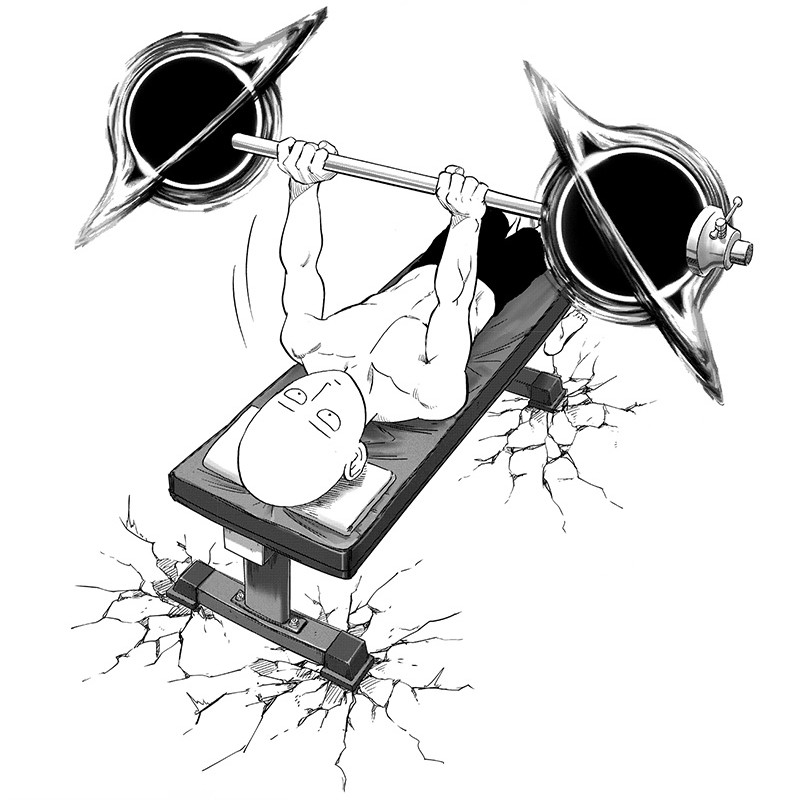
\includegraphics[width=\linewidth]{images/saitama_blackholes.jpg}%
\end{center}\bigskip}

\makeatletter\newcommand*{\atf}{
\includegraphics[totalheight=\heightof{@}]{pglpm_latex/atblack.png}}\makeatother
% \providecommand{\affiliation}[1]{\textsl{\textsf{\footnotesize #1}}}
\providecommand{\epost}[1]{\texttt{\footnotesize\textless#1\textgreater}}
\providecommand{\email}[2]{\href{mailto:#1ZZ@#2 ((remove ZZ))}{#1\protect\atf#2}}
%\providecommand{\email}[2]{\href{mailto:#1@#2}{#1@#2}}

\preauthor{\begin{center}%\color{white}%
\Large\sffamily%
}
\postauthor{\par\end{center}}
\predate{\DTMsetdatestyle{mydate}\begin{center}\footnotesize%\color{white}%
}
\postdate{\par\end{center}}

\setfloatadjustment{figure}{\footnotesize}
\captiondelim{\quad}
\captionnamefont{\footnotesize\sffamily%
}
\captiontitlefont{\footnotesize}
%\firmlists*
\midsloppy
% handling orphan/widow lines, memman.pdf
% \clubpenalty=10000
% \widowpenalty=10000
% \raggedbottom
% Downes, memman.pdf
\clubpenalty=9996
\widowpenalty=9999
\brokenpenalty=4991
\predisplaypenalty=10000
\postdisplaypenalty=1549
\displaywidowpenalty=1602
\raggedbottom

\paragraphfootnotes
\setlength{\footmarkwidth}{2ex}
% \threecolumnfootnotes
%\setlength{\footmarksep}{0em}
\footmarkstyle{\textsuperscript{%\color{red}
\scriptsize\bfseries#1}~}
%\footmarkstyle{\textsuperscript{\color{red}\scriptsize\bfseries#1}~}
%\footmarkstyle{\textsuperscript{[#1]}~}

\selectlanguage{british}\frenchspacing
\usepackage{fontawesome5}

% \usepackage{wrapfig2}
% \newlength{\wfwidth}
% \setlength{\wfwidth}{0.4\linewidth}

\colorlet{mpcolor}{green}
%\newcommand*{\puzzle}{\maltese}
% \newcommand*{\puzzle}{{\fontencoding{U}\fontfamily{fontawesometwo}\selectfont\symbol{225}}}
% \newcommand*{\wrench}{{\fontencoding{U}\fontfamily{fontawesomethree}\selectfont\symbol{114}}}
% \newcommand*{\pencil}{{\fontencoding{U}\fontfamily{fontawesometwo}\selectfont\symbol{210}}}
\newcommand{\mynotew}[1]{{\footnotesize\color{midgrey}\faIcon{tools}\ #1}}
% \newcommand{\mynotep}[1]{{\footnotesize\color{notecolour}\pencil\ #1}}
% \newcommand{\mynotez}[1]{{\footnotesize\color{notecolour}\puzzle\ #1}}

%%%%%%%%%%%%%%%%%%%%%%%%%%%%%%%%%%%%%%%%%%%%%%%%%%%%%%%%%%%%%%%%%%%%%%%%%%%%
%%% Paper's details
%%%%%%%%%%%%%%%%%%%%%%%%%%%%%%%%%%%%%%%%%%%%%%%%%%%%%%%%%%%%%%%%%%%%%%%%%%%%
\title{\propertitle}
\ifanon\else\author{%
\hspace*{\stretch{1}}%
%% uncomment if additional authors present
% \parbox{0.5\linewidth}%\makebox[0pt][c]%
% {\protect\centering ***\\%
% \footnotesize\epost{\email{***}{***}}}%
% \hspace*{\stretch{1}}%
\parbox{1\linewidth}%\makebox[0pt][c]%
{\protect\centering P.G.L.  Porta\,Mana
 %\href{https://orcid.org/0000-0002-6070-0784}{\raisebox{0.5ex}{\protect
\includegraphics[height=1ex]{pglpm_latex/orcid_32x32.png}}}%
% \\\footnotesize
% Western Norway University of Applied Sciences%
% \quad\epost{\email{pgl}{portamana.org}}%
}%
%% uncomment if additional authors present
% \hspace*{\stretch{1}}%
% \parbox{0.5\linewidth}%\makebox[0pt][c]%
% {\protect\centering ***\\%
% \footnotesize\epost{\email{***}{***}}}%
\hspace*{\stretch{1}}%
}\fi

%\date{Draft of \today\ (first drafted \firstdraft)}
\date{%\textbf{Working draft} version \version, updated
Updated \updated%\\[\jot]\href{https://pglpm.github.io/7wonders/}{pglpm.github.io/7wonders}
}

%%%%%%%%%%%%%%%%%%%%%%%%%%%%%%%%%%%%%%%%%%%%%%%%%%%%%%%%%%%%%%%%%%%%%%%%%%%%
%%% Macros @@@
%%%%%%%%%%%%%%%%%%%%%%%%%%%%%%%%%%%%%%%%%%%%%%%%%%%%%%%%%%%%%%%%%%%%%%%%%%%%

% Common ones - uncomment as needed
%\providecommand{\nequiv}{\not\equiv}
%\providecommand{\coloneqq}{\mathrel{\mathop:}=}
%\providecommand{\eqqcolon}{=\mathrel{\mathop:}}
%\providecommand{\varprod}{\prod}
\newcommand*{\de}{\mathop{}\!\uppartial}%partial diff
\newcommand*{\pu}{\piup}%constant pi
\newcommand*{\delt}{\deltaup}%Kronecker, Dirac
%\newcommand*{\eps}{\varepsilonup}%Levi-Civita, Heaviside
%\newcommand*{\riem}{\zetaup}%Riemann zeta
%\providecommand{\degree}{\textdegree}% degree
%\newcommand*{\celsius}{\textcelsius}% degree Celsius
%\newcommand*{\micro}{\textmu}% degree Celsius
% \newcommand*{\I}{\mathrm{i}}%imaginary unit
\newcommand*{\I}{\ensuremath{\mathrm{i}}}
% \newcommand*{\e}{\mathrm{e}}%Neper
\newcommand*{\e}{\ensuremath{\mathrm{e}}}
% See https://tex.stackexchange.com/a/84308/97039
\newcommand*{\di}{\mathop{}\!\mathrm{d}}%differential
% \newcommand*{\dii}{\ensuremath{\mathrm{d}}}
% %% From TUGboat 18 (1997) 1 - leads to very strange spacing
% \makeatletter
% \providecommand*{\di}%
% {\@ifnextchar^{\DIfF}{\DIfF^{}}}
% \def\DIfF^#1{%
% \mathop{\mathrm{\mathstrut d}}%
% \nolimits^{#1}\gobblespace}
% \def\gobblespace{%
% \futurelet\diffarg\opspace}
% \def\opspace{%
% \let\DiffSpace\!%
% \ifx\diffarg(%
% \let\DiffSpace\relax
% \else
% \ifx\diffarg[%
% \let\DiffSpace\relax
% \else
% \ifx\diffarg\{%
% \let\DiffSpace\relax
% \fi\fi\fi\DiffSpace}
% \makeatother

% \newcommand*{\Di}{\mathop{}\!\mathrm{D}}%capital differential
%\newcommand*{\Li}{\mathop{}\!\mathrm{L}}%Lie derivative
%\newcommand*{\planckc}{\hslash}
%\newcommand*{\avogn}{N_{\textrm{A}}}
%\newcommand*{\NN}{\bm{\mathrm{N}}}
%\newcommand*{\ZZ}{\bm{\mathrm{Z}}}
%\newcommand*{\QQ}{\bm{\mathrm{Q}}}
\newcommand*{\RR}{\bm{\mathrm{R}}}
%\newcommand*{\CC}{\bm{\mathrm{C}}}
%\newcommand*{\nabl}{\bm{\nabla}}%nabla
%\DeclareMathOperator{\lb}{lb}%base 2 log
%\DeclareMathOperator{\tr}{tr}%trace
%\DeclareMathOperator{\card}{card}%cardinality
%% From TUGboat 18 (1997) 1
% \renewoperator{\Re}{\mathrm{Re}}{\nolimits}
% \renewoperator{\Im}{\mathrm{Im}}{\nolimits}
\DeclareMathOperator{\im}{Im}%im part
\DeclareMathOperator{\re}{Re}%re part
%\DeclareMathOperator{\sgn}{sgn}%signum
%\DeclareMathOperator{\ent}{ent}%integer less or equal to
%\DeclareMathOperator{\Ord}{O}%same order as
%\DeclareMathOperator{\ord}{o}%lower order than
% \newcommand*{\incr}{\triangle}%finite increment
\newcommand*{\incr}{\Delta}%finite increment
\newcommand*{\defd}{\coloneqq}
\newcommand*{\defs}{\eqqcolon}
%\newcommand*{\Land}{\bigwedge}
%\newcommand*{\Lor}{\bigvee}
%\newcommand*{\lland}{\DOTSB\;\land\;}
%\newcommand*{\llor}{\DOTSB\;\lor\;}
\newcommand*{\limplies}{\mathbin{\Rightarrow}}%implies
%\newcommand*{\suchthat}{\mid}%{\mathpunct{|}}%such that (eg in sets)
%\newcommand*{\with}{\colon}%with (list of indices)
%\newcommand*{\mul}{\times}%multiplication
%\newcommand*{\inn}{\cdot}%inner product
%\newcommand*{\dotv}{\mathord{\,\cdot\,}}%variable place
%\newcommand*{\comp}{\circ}%composition of functions
%\newcommand*{\con}{\mathbin{:}}%scal prod of tensors
%\newcommand*{\equi}{\sim}%equivalent to
\renewcommand*{\asymp}{\simeq}%equivalent to
%\newcommand*{\corr}{\mathrel{\hat{=}}}%corresponds to
%\providecommand{\varparallel}{\ensuremath{\mathbin{/\mkern-7mu/}}}%parallel (tentative symbol)
% \renewcommand*{\le}{\leqslant}%less or equal
% \renewcommand*{\ge}{\geqslant}%greater or equal
\DeclarePairedDelimiter\clcl{[}{]}
\DeclarePairedDelimiter\clop{[}{[}
\DeclarePairedDelimiter\opcl{]}{]}
\DeclarePairedDelimiter\opop{]}{[}%}
\DeclarePairedDelimiter\abs{\lvert}{\rvert}
%\DeclarePairedDelimiter\norm{\lVert}{\rVert}
\DeclarePairedDelimiter\set{\{}{\}} %}
%\DeclareMathOperator{\pr}{P}%probability
\newcommand*{\p}{\mathrm{p}}%probability
\renewcommand*{\P}{\mathrm{P}}%probability
%\newcommand*{\E}{\mathrm{E}}
%% The "\:" space is chosen to correctly separate inner binary and external rels
\renewcommand*{\|}[1][]{\nonscript\:#1\vert\nonscript\:\mathopen{}}
%\DeclarePairedDelimiterX{\cp}[2]{(}{)}{#1\nonscript\:\delimsize\vert\nonscript\:\mathopen{}#2}
%\DeclarePairedDelimiterX{\ct}[2]{[}{]}{#1\nonscript\;\delimsize\vert\nonscript\:\mathopen{}#2}
%\DeclarePairedDelimiterX{\cs}[2]{\{}{\}}{#1\nonscript\:\delimsize\vert\nonscript\:\mathopen{}#2}
%\newcommand*{\+}{\lor}
%\renewcommand{\*}{\land}
%% symbol = for equality statements within probabilities
%% from https://tex.stackexchange.com/a/484142/97039
% \newcommand*{\eq}{\mathrel{\!=\!}}
% \let\texteq\=
% \renewcommand*{\=}{\TextOrMath\texteq\eq}
% \newcommand*{\eq}[1][=]{\mathrel{\!#1\!}}
\newcommand*{\mo}[1][=]{\mathclose{}\mathord{\nonscript\mkern0.5mu#1\nonscript\mkern0.5mu}\mathopen{}}
%%
\newcommand*{\sect}{\S}% Sect.~
\newcommand*{\sects}{\S\S}% Sect.~
\newcommand*{\chap}{Chapter}%
\newcommand*{\chaps}{chs}%
\newcommand*{\bref}{ref.}%
\newcommand*{\brefs}{refs}%
%\newcommand*{\fn}{fn}%
\newcommand*{\eqn}{eq.}%
\newcommand*{\eqns}{eqs}%
\newcommand*{\fig}{fig.}%
\newcommand*{\figs}{figs}%
\newcommand*{\vs}{{vs}}
\newcommand*{\eg}{{e.g.}}
\newcommand*{\etc}{{etc.}}
\newcommand*{\ie}{{i.e.}}
%\newcommand*{\ca}{{c.}}
\newcommand*{\foll}{{ff.}}
%\newcommand*{\viz}{{viz}}
\newcommand*{\cf}{{cf.}}
%\newcommand*{\Cf}{{Cf.}}
%\newcommand*{\vd}{{v.}}
\newcommand*{\etal}{{et al.}}
%\newcommand*{\etsim}{{et sim.}}
%\newcommand*{\ibid}{{ibid.}}
%\newcommand*{\sic}{{sic}}
%\newcommand*{\id}{\mathte{I}}%id matrix
%\newcommand*{\nbd}{\nobreakdash}%
%\newcommand*{\bd}{\hspace{0pt}}%
%\def\hy{-\penalty0\hskip0pt\relax}
%\newcommand*{\labelbis}[1]{\tag*{(\ref{#1})$_\text{r}$}}
%\newcommand*{\mathbox}[2][.8]{\parbox[t]{#1\columnwidth}{#2}}
\newcommand*{\zerob}[1]{\makebox[0pt][c]{#1}}
\newcommand*{\tprod}{\mathop{\textstyle\prod}\nolimits}
\newcommand*{\tsum}{\mathop{\textstyle\sum}\nolimits}
%\newcommand*{\tint}{\begingroup\textstyle\int\endgroup\nolimits}
%\newcommand*{\tland}{\mathop{\textstyle\bigwedge}\nolimits}
%\newcommand*{\tlor}{\mathop{\textstyle\bigvee}\nolimits}
%\newcommand*{\sprod}{\mathop{\textstyle\prod}}
%\newcommand*{\ssum}{\mathop{\textstyle\sum}}
%\newcommand*{\sint}{\begingroup\textstyle\int\endgroup}
%\newcommand*{\sland}{\mathop{\textstyle\bigwedge}}
%\newcommand*{\slor}{\mathop{\textstyle\bigvee}}
%\newcommand*{\T}{^\transp}%transpose
%%\newcommand*{\QEM}%{\textnormal{$\Box$}}%{\ding{167}}
%\newcommand*{\qem}{\leavevmode\unskip\penalty9999 \hbox{}\nobreak\hfill
%\quad\hbox{\QEM}}
%% from TUGboat 18 (1997) 1:
%\providecommand*{\unit}[1]{\ensuremath{\mathrm{\,#1}}}

%%%%%%%%%%%%%%%%%%%%%%%%%%%%%%%%%%%%%%%%%%%%%%%%%%%%%%%%%%%%%%%%%%%%%%%%%%%%
%%% Custom macros for this file @@@
%%%%%%%%%%%%%%%%%%%%%%%%%%%%%%%%%%%%%%%%%%%%%%%%%%%%%%%%%%%%%%%%%%%%%%%%%%%%

\newcommand*{\widebar}[1]{{\mkern1.5mu\skew{2}\overline{\mkern-1.5mu#1\mkern-1.5mu}\mkern 1.5mu}}

% \newcommand{\explanation}[4][t]{%\setlength{\tabcolsep}{-1ex}
% %\smash{
% \begin{tabular}[#1]{c}#2\\[0.5\jot]\rule{1pt}{#3}\\#4\end{tabular}}%}
% \newcommand*{\ptext}[1]{\text{\small #1}}% for propositions
% \DeclareMathOperator*{\argsup}{arg\,sup}
\newcommand*{\furl}[2]{\href{#1}{#2}\,\pagenote{\url{#1}}}
% \renewcommand*{\autoref}[3][\sect~\ref]{\sidepar{\vspace{-1ex}\footnotesize{\color{blue}\faIcon{angle-right}\enskip#1{#2} page~\pageref{#2}}}\textcolor{blue}{#3}}
\renewcommand*{\autoref}[3][\sect\,\ref]{\textcolor{blue}{#3} {\color{blue}\scriptsize(\faIcon{angle-right}~#1{#2}\;p.\,\pageref{#2})}}
% %hand-point-right%
% %undo%
% %undo-alt%
% %reply%
% %history%

%% auxiliary
\newcommand*{\energym}{energy-mass}
\newcommand*{\masse}{mass-energy}
\newcommand*{\tot}{_{\textrm{tot}}}

\newcommand{\textdim}{\textsf}

%% constants
%% R % molar gas constant
\newcommand*{\yc}{c} % lightspeed, according to SI
% \newcommand*{\yc}{c_{0}} % lightspeed, according to SI
\newcommand*{\yfri}{\mu} % friction coeff
\newcommand*{\yfris}{\mu_{\text{s}}}
\newcommand*{\yfrik}{\mu_{\text{k}}}
\newcommand*{\yvis}{\mu} % viscosity coeff
\newcommand*{\yhea}{h} % heat-transfer coeff
\newcommand*{\yg}{\bm{g}} % gravitational acceleration
\newcommand*{\yh}{\bm{h}} % gravitational-inertial-magnetic force
\newcommand*{\yGG}{\kappa} % gravitational constant


%% time and space
\newcommand*{\ye}{\bm{e}} % unit vector
\newcommand*{\yuu}{\bm{u}}
\newcommand*{\yww}{\bm{w}}
\newcommand*{\yr}{\bm{r}}
\newcommand*{\yra}{\yr_{a}}
\newcommand*{\yrb}{\yr_{b}}
\newcommand*{\yxa}{x_{a}}%
\newcommand*{\yxb}{x_{b}}%
\newcommand*{\yv}{\bm{v}}
\newcommand*{\yva}{\yv_{a}}
\newcommand*{\yvb}{\yv_{b}}
\newcommand*{\yvs}{\bm{v}_{\text{s}}}
\newcommand*{\yns}{\bm{n}_{\text{s}}}
\newcommand*{\yst}{\bm{\sigma}}
\newcommand*{\ylo}{l_{\textrm{n}}}
\newcommand*{\yle}{l}
\newcommand*{\ydl}{\incr\bm{l}}
\newcommand*{\ydlm}{\incr l}
\newcommand*{\yti}{t_{0}}
\newcommand*{\ytf}{t_{1}}
\newcommand*{\yxi}{x_{0}}
\newcommand*{\yyi}{y_{0}}
\newcommand*{\yzi}{z_{0}}
\newcommand*{\dt}{\di t}
\newcommand*{\Dt}{\incr t}
\newcommand*{\Dx}{\incr x}
\newcommand*{\Dy}{\incr y}
\newcommand*{\Dz}{\incr z}
\newcommand*{\Dth}{\tfrac{\incr t}{2}}
\newcommand*{\Dxh}{\tfrac{\incr x}{2}}
\newcommand*{\Dyh}{\tfrac{\incr y}{2}}
\newcommand*{\Dzh}{\tfrac{\incr z}{2}}

%% matter
\newcommand*{\yN}{N}
\newcommand*{\yJ}{J}
\newcommand*{\yn}{n}
\newcommand*{\yj}{\bm{j}}
% \newcommand*{\ya}{\varAlpha}
\newcommand*{\ya}{\mathcal{A}}
\newcommand*{\yrho}{\rho}
\newcommand*{\yNu}{\yN_{\text{u}}}
\newcommand*{\yNv}{\yN_{\text{v}}}
\newcommand*{\yJu}{\yJ_{\text{u}}}
\newcommand*{\yJv}{\yJ_{\text{v}}}
\newcommand*{\yau}{\ya_{\text{u}}}
\newcommand*{\yav}{\ya_{\text{v}}}

%% energy
\newcommand*{\ym}{m}% m, and q_m for mass flow
\newcommand*{\yma}{\ym_{a}}
\newcommand*{\ymb}{\ym_{b}}
\newcommand*{\yE}{E}
\newcommand*{\yU}{U}
\newcommand*{\yUd}{u}
\newcommand*{\yUr}{U_{\textrm{new}}}
\newcommand*{\yUo}{\yU_{0}}
\newcommand*{\yEk}{\yE_{\textrm{k}}}%T
\newcommand*{\yEp}{\yE_{\textrm{p}}}%V
\newcommand*{\yH}{\varPhi}% really used for heat-flow
\newcommand*{\yHs}{\yH_{s}}%
% \newcommand*{\yEp}{\yE_{\text{p}}}
\newcommand*{\yHfl}{\yH_{\textrm{floor}}}
\newcommand*{\yHc}{\yH_{\textrm{crate}}}
\newcommand*{\yQ}{Q}% Q really for time-integral
\newcommand*{\yQb}{Q_{\textrm{bot}}}%
\newcommand*{\yQp}{\yQ^{+}}%
\newcommand*{\yQm}{\yQ^{-}}%
\newcommand*{\yQc}{\yQ_{\textrm{crate}}}
\newcommand*{\yQfl}{\yQ_{\textrm{floor}}}
\newcommand*{\yhe}{\incr H}% integrated heat flux
\newcommand*{\yhep}{\incr H^{+}}%
\newcommand*{\yhem}{\incr H^{-}}%
\newcommand*{\yW}{\incr W}% work
\newcommand*{\yR}{\mathcal{R}}% for energy source

%% momentum
\newcommand*{\yP}{\bm{P}}
\newcommand*{\yPa}{\yP_{a}}
\newcommand*{\yPb}{\yP_{b}}
\newcommand*{\yp}{\bm{p}}
\newcommand*{\yF}{\bm{F}}
\newcommand*{\yFab}{\yF_{as}}
\newcommand*{\yFba}{\yF_{bs}}
\newcommand*{\yFa}{\yF_{a}}
\newcommand*{\yFb}{\yF_{b}}
\newcommand*{\yFpg}{F_{\text{pg}}}
\newcommand*{\yFgp}{F_{\text{gp}}}
\newcommand*{\yFatm}{F_{\text{atm}}}
\newcommand*{\yFc}{\yF_{\text{c}}}
\newcommand*{\yFn}{F_{\text{n}}}
\newcommand*{\yFs}{F_{\text{s}}}
\newcommand*{\yFk}{\yF_{\text{k}}}
\newcommand*{\yFr}{\yF_{\text{other}}}
\newcommand*{\yFrx}{F_{\text{other},x}}
\newcommand*{\yFrz}{F_{\text{other},z}}
\newcommand*{\yFp}{F_{\text{p}}}
\newcommand*{\yFf}{F_{\text{f}}}
\newcommand*{\ypr}{p} % pressure
\newcommand*{\ypv}{\bm{\ypr}} % pressure vector
\newcommand*{\yG}{\bm{G}}
\newcommand*{\yGa}{\yG_{a}}
\newcommand*{\yGb}{\yG_{b}}

%% rigid motion
\newcommand*{\yOm}{\bm{\varOmega}}
\newcommand*{\yo}{\bm{\omega}}
\newcommand*{\yox}{\omega_{x}}
\newcommand*{\yoy}{\omega_{y}}
\newcommand*{\yoz}{\omega_{z}}
\newcommand*{\yro}{\yr_{0}}
\newcommand*{\yrcm}{\yr_{\textrm{c}}}
\newcommand*{\yxcm}{x_{\textrm{c}}}
\newcommand*{\yycm}{y_{\textrm{c}}}
\newcommand*{\yzcm}{z_{\textrm{c}}}
\newcommand*{\yvcm}{\yv_{\textrm{c}}}
\newcommand*{\yvxcm}{\dot{x}_{\textrm{c}}}
\newcommand*{\yvycm}{\dot{y}_{\textrm{c}}}
\newcommand*{\yvzcm}{\dot{z}_{\textrm{c}}}
\newcommand*{\yIc}{\bm{I}_{\textrm{c}}}

%% angular momentum
\newcommand*{\yL}{\bm{L}}% L or H
%\newcommand*{\yl}{\bm{L}}
% \newcommand*{\yto}{\bm{\varTau}}% volume torque M or T or M_Q
\newcommand*{\ytoo}{\mathcal{T}}% volume torque M or T or M_Q
\newcommand*{\yto}{\bm{\ytoo}}% volume torque M or T or M_Q
\newcommand*{\yM}{\bm{M}}% surface torque M or T or M_Q
%\newcommand*{\yt}{\bm{\tau}}

%% entropy and temperature
\newcommand*{\yS}{S}
\newcommand*{\yB}{\varPi}
\newcommand*{\yT}{T}%temperature
\newcommand*{\yTce}{T_{\text{C}}}%
\newcommand*{\yTp}{\yT^{+}}%
\newcommand*{\yTm}{\yT^{-}}%
\newcommand*{\yTa}{\yT_{a}}%
\newcommand*{\yTb}{\yT_{b}}%
\newcommand*{\yTe}{\yT_{\text(ext)}}%

%% electric charge and magnetic flux
\newcommand*{\yC}{\mathcal{Q}}
\newcommand*{\yI}{\mathcal{I}}
\newcommand*{\yBf}{\mathcal{B}}
\newcommand*{\yEv}{\mathcal{E}}
\newcommand*{\yBB}{\bm{B}}
\newcommand*{\yEE}{\bm{E}}

\newcommand*{\cx}[1]{x_{\text{#1}}}
\newcommand*{\cy}[1]{y_{\text{#1}}}
\newcommand*{\cz}[1]{z_{\text{#1}}}
\newcommand*{\vx}[1]{\dot{x}_{\text{#1}}}
\newcommand*{\vy}[1]{\dot{y}_{\text{#1}}}
\newcommand*{\vz}[1]{\dot{z}_{\text{#1}}}
\newcommand*{\ax}[1]{\ddot{x}_{\text{#1}}}
\newcommand*{\ay}[1]{\ddot{y}_{\text{#1}}}
\newcommand*{\az}[1]{\ddot{z}_{\text{#1}}}

%%% Custom macros end @@@

% % https://latex.org/forum/viewtopic.php?t=878
% \newenvironment{widepar}%
% {\setlength{\rightskip}{-\marginparsep}\addtolength{\rightskip}{-\marginparwidth}}{\par}


\usepackage[%
print-unity-mantissa=true,%
parse-units=false,%
%exponent-product=\cdot,%
%quantity-product=\:,%
retain-explicit-plus,%
]{siunitx}
%\sisetup{input-digits = 0123456789\piup}

\colorlet{codecolour}{blue}
\usepackage{listings}
\lstdefinestyle{mycode}{
  basicstyle=\ttfamily\footnotesize\bfseries\color{codecolour},
  moredelim=**[is][\color{grey}]{\%@}{\%@},
  frame=single,
  numbers=left,
  numberstyle=\sffamily\scriptsize,
  xleftmargin=\parindent
}

% \usepackage{multimedia}
\usepackage[breakable,skins]{tcolorbox}

% \newtcolorbox{myframe}{enhanced, no shadow, colback=white, colframe=midgrey, boxrule=1pt, breakable, after={\smallskip}}

\newtcolorbox{solution}{enhanced, no shadow,
  %colback=green!5!white,
  interior hidden,
  borderline west={1pt}{0pt}{midgrey},
  borderline south={1pt}{0pt}{midgrey!25!white},
  frame hidden,
  left=1ex, right=0ex, bottom=1ex,
  fontupper=\color{midgrey},
  %colframe=green,
  %leftrule=0pt, rightrule=0pt, bottomrule=0.5pt, toprule=0pt,
  breakable, fonttitle=\bfseries\sffamily, after={\smallskip},
  title=\color{midgrey}Example solution}
%map-marker-alt


% \newtcolorbox[auto counter, number within=chapter]{exercise}[1][]{enhanced,
%   no shadow,
%   %parbox=false,
%   % colback=yellow!5!white, colframe=yellow, boxrule=1pt,
%   interior hidden,
%   borderline west={1pt}{0pt}{yellow},
%   borderline south={1pt}{0pt}{yellow!25!white},
%   frame hidden,
%   left=1ex, right=0ex, bottom=1ex,
%   breakable,
%   % fontupper=\small,
%   fonttitle=\bfseries\sffamily,
%   after={\smallskip},
%   title=\color{yellow}\faIcon{puzzle-piece}\enskip Exercise~\thetcbcounter,#1}
% 
% \newtcolorbox{warning}[1][]{enhanced, no shadow,
%   %parbox=false,
%   % colback=red!5!white,
%   % colframe=red, left=1ex, right=1ex, leftrule=0pt, rightrule=0pt, bottomrule=0.5pt, toprule=0pt,
%   interior hidden,
%   borderline west={1pt}{0pt}{red},
%   borderline south={1pt}{0pt}{red!25!white},
%   frame hidden,
%   left=1ex, right=0ex, bottom=1ex,
%   breakable,
% % fontupper=\small, fonttitle=\bfseries\small,
% fonttitle=\bfseries,
% after={\smallskip},
% title=\color{red}\faIcon{exclamation-circle}\enskip#1}
% 
% % \newtcolorbox{critique}[1][Critique]{enhanced, no shadow,parbox=false,center,
% % width=0.9\linewidth, colback=blue!5!white, colframe=blue, boxrule=1pt, breakable, fontupper=\small, fonttitle=\bfseries\small, after={\smallskip}, title=\hspace{-2ex}\faIcon{microscope}\enskip#1}
% 
% \newtcolorbox{definition}[1]{enhanced, no shadow,
%   %colback=green!5!white,
%   interior hidden,
%   borderline west={1pt}{0pt}{green},
%   borderline south={1pt}{0pt}{green!25!white},
%   frame hidden,
%   left=1ex, right=0ex, bottom=1ex,
%   %colframe=green,
%   %leftrule=0pt, rightrule=0pt, bottomrule=0.5pt, toprule=0pt,
%   breakable, fonttitle=\bfseries\sffamily, after={\smallskip}, title=\color{green}\faIcon{bookmark}\enskip#1}
% %map-marker-alt
% 
% \newtcolorbox{extra}[1]{enhanced, no shadow,
%   %parbox=false, %width=0.975\linewidth,
%   % center, colback=blue!5!white, colframe=blue, boxrule=0.5pt,
%   interior hidden,
%   borderline west={1pt}{0pt}{blue},
%   borderline south={1pt}{0pt}{blue!25!white},
%   frame hidden,
%   left=1ex, right=0ex, bottom=1ex,
%   breakable,
%    fontupper=\footnotesize,
%   fonttitle=\bfseries\sffamily\footnotesize, after={\smallskip}, title=\color{blue}\faIcon{user-astronaut}\enskip#1}
% \newtcolorbox[auto counter, number within=chapter]{extra}[2][]{enhanced, no shadow, parbox=false,width=0.975\linewidth, flush right, colback=blue!5!white, colframe=blue, boxrule=0.5pt, breakable, fontupper=\small, fonttitle=\bfseries\small, after={\smallskip}, title=\hspace{-2ex}\faIcon{rocket}\enskip Curiosity~\thetcbcounter\enskip#2,#1}

%%%%%%%%%%%%%%%%%%%%%%%%%%%%%%%%%%%%%%%%%%%%%%%%%%%%%%%%%%%%%%%%%%%%%%%%%%%%
%%% Beginning of document
%%%%%%%%%%%%%%%%%%%%%%%%%%%%%%%%%%%%%%%%%%%%%%%%%%%%%%%%%%%%%%%%%%%%%%%%%%%%
% \firmlists

% \setlength{\wrapoverhang}{\parindent}
% \setlength{\intextsep}{1ex}% with wrapfigure
% % \setlength{\columnsep}{2em}% with wrapfigure

\makepagenote
\renewcommand*{\notedivision}{}
\renewcommand*{\pagenotesubhead}[3]{\clearpage\addsec{URLs for chapter #2}}
\renewcommand*{\pagenotesubheadstarred}[3]{\clearpage\addsec{URLs for chapter \textit{#3}}}
\renewcommand*{\notenuminnotes}[1]{\footnotesize #1.\space}
% \renewcommand{\prenotetext}{\begingroup\footnotesize}
% \renewcommand{\postnotetext}{\endgroup}
\sideparmargin{right}

% \newlength{\pagewidth}
% \setlength{\pagewidth}{\linewidth}
% \addtolength{\pagewidth}{\marginparsep}
% \addtolength{\pagewidth}{\marginparwidth}

%\usepackage{cancel}

% \usepackage{eso-pic}
% \newcommand\BackgroundPic{%
% \put(0,0){%
% \parbox[b][\paperheight]{\paperwidth}{%
% \vfill
% \centering
% 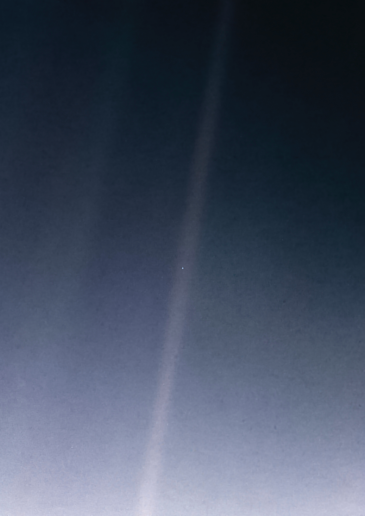
\includegraphics[width=\paperwidth,height=\paperheight,%
% keepaspectratio]{images/palebluedotA4s.png}%
% \vfill
% }}}

%\usepackage[6-73,105-107]{pagesel}
\usepackage{tikz}
\usetikzlibrary{tikzmark}
\usetikzlibrary{arrows.meta}
% \usetikzlibrary{positioning}
% \newcommand{\tikzmark}[1]{\tikz[overlay,remember picture] \node (#1) {};}

\begin{document}
%\AddToShipoutPicture*{\BackgroundPic}
\captiondelim{\quad}\captionnamefont{\footnotesize}\captiontitlefont{\footnotesize}
\selectlanguage{british}\frenchspacing

\begin{titlingpage}
\calccentering{\unitlength}
\begin{adjustwidth}{\unitlength}{-\unitlength}
  \centering
  % c6ddff % color of Earth in the Pale Blue Dot picture
% \color[HTML]{C6DDFF}
 \color[HTML]{354055}
  \maketitle
\end{adjustwidth}
\end{titlingpage}
\killtitle

\calccentering{\unitlength}
\begin{adjustwidth*}{\unitlength}{-\unitlength}\thispagestyle{empty}
  \centering
  
\includegraphics[align=c,height=1em]{images/cc_by_sa.png} Licence

  \medskip
  P.G.L. Porta Mana \enskip\epost{\email{pgl}{portamana.org}}
  \\\href{https://orcid.org/0000-0002-6070-0784}{%
%\raisebox{0.5ex}{\protect%

\includegraphics[height=1ex]{pglpm_latex/orcid_32x32.png}%}
}%
\,{\footnotesize\url{https://orcid.org/0000-0002-6070-0784}}

\medskip

Typeset with \LaTeX.%\ using 12\,pt Palatino and Optima fonts

\medskip

No large language models were used in the production of this document.

\bigskip

Cover image: adapted from \href{https://onepunchman.fandom.com}{\emph{One Punch Man}} Punch~192: \href{https://onepunchman.fandom.com/wiki/Chapter_192_(Online)}{\emph{Level Up}}.
\end{adjustwidth*}
\setcounter{page}{2}

% \calccentering{\unitlength}
% \begin{adjustwidth*}{\unitlength}{-\unitlength}\thispagestyle{empty}
%   \centering
%   
\includegraphics[align=c,height=1em]{images/cc_by_sa.png} Licence
% 
%   \smallskip
% 
%   %%% ***%%% Luca\enskip\href{https://orcid.org/0000-0002-6070-0784}{\raisebox{0.5ex}{\protect
\includegraphics[height=1ex]{pglpm_latex/orcid_32x32.png}}}{\footnotesize\url{https://orcid.org/0000-0002-6070-0784}}
% 
% \smallskip
% 
% Typeset with \LaTeX%\ using 12\,pt Palatino and Optima fonts
% 
% \bigskip
% 
% % Cover image: the \enquote{Pale Blue Dot} image of the Earth taken by Voyager~1,
% % \\from right outside Pluto's orbit\\
% % \url{https://science.nasa.gov/resource/voyager-1s-pale-blue-dot/}
% \end{adjustwidth*}
\setcounter{page}{2}


%%%%%%%%%%%%%%%%%%%%%%%%%%%%%%%%%%%%%%%%%%%%%%%%%%%%%%%%%%%%%%%%%%%%%%%%%%%%
%%% Abstract
%%%%%%%%%%%%%%%%%%%%%%%%%%%%%%%%%%%%%%%%%%%%%%%%%%%%%%%%%%%%%%%%%%%%%%%%%%%%
% \abstractrunin
% \abslabeldelim{}
% \renewcommand*{\abstractname}{}
% \setlength{\absleftindent}{0pt}
% \setlength{\absrightindent}{0pt}
% \setlength{\abstitleskip}{-\absparindent}
% \begin{abstract}\labelsep 0pt%
%   \noindent Lecture notes on introductory mechanics and thermodynamics (ING175)
% % \\\noindent\emph{\footnotesize Note: Dear Reader
% %     \amp\ Peer, this manuscript is being peer-reviewed by you. Thank you.}
% % \par%\\[\jot]
% % \noindent
% % {\footnotesize PACS: ***}\qquad%
% % {\footnotesize MSC: ***}%
% %\qquad{\footnotesize Keywords: ***}
% \end{abstract}
\selectlanguage{british}\frenchspacing

%%%%%%%%%%%%%%%%%%%%%%%%%%%%%%%%%%%%%%%%%%%%%%%%%%%%%%%%%%%%%%%%%%%%%%%%%%%%
%%% Epigraph
%%%%%%%%%%%%%%%%%%%%%%%%%%%%%%%%%%%%%%%%%%%%%%%%%%%%%%%%%%%%%%%%%%%%%%%%%%%%
% \asudedication{\small ***}
% \vspace{\bigskipamount}
\setlength{\epigraphwidth}{0.67\linewidth}
% \epigraphtextposition{flushright}
% %\epigraphsourceposition{flushright}
\epigraphfontsize{\footnotesize}
\setlength{\epigraphrule}{0pt}
% % \epigraphposition{flushright}
% %\setlength{\beforeepigraphskip}{0pt}
%\setlength{\afterepigraphskip}{2em}



%%%%%%%%%%%%%%%%%%%%%%%%%%%%%%%%%%%%%%%%%%%%%%%%%%%%%%%%%%%%%%%%%%%%%%%%%%%%
%%% BEGINNING OF MAIN TEXT
%%%%%%%%%%%%%%%%%%%%%%%%%%%%%%%%%%%%%%%%%%%%%%%%%%%%%%%%%%%%%%%%%%%%%%%%%%%%
% \renewcommand{\cftchapterfont}{\hfill\bfseries}
% \renewcommand{\cftchapterleader}{}
% \renewcommand{\cftsectionfont}{\hfill\normalfont}
% \renewcommand{\cftcsectionleader}{}

\cleartooddpage
\phantomsection\pdfbookmark{\contentsname}{toc}
\setlength{\cftsectionnumwidth}{2.75em}
\tableofcontents*
\label{sec:toc}

\setcounter{chapter}{0}


%%%%%%%%%%%%%%%%%%%%%%%%%%%%%%%%%%%%%%%%%%%%%%%%%%%%%%%%%%%%%%%%%%%%%%%%%%%%
%%% Preface
%%%%%%%%%%%%%%%%%%%%%%%%%%%%%%%%%%%%%%%%%%%%%%%%%%%%%%%%%%%%%%%%%%%%%%%%%%%%
% \printpagenotes*
% \cleartooddpage
% \addchap{Preface}
% \label{cha:preface}



% \printpagenotes*
% \cleartooddpage
% \chapter{Overview}
% \label{cha:overview}



\printpagenotes*
\cleartooddpage
\chapter{Physics, quantities, units}
\label{cha:physics_quantities_units}
\setcounter{section}{-1}

For some of the following exercises you can refer to tables~\ref{tab:units} and \ref{tab:symbols_volint_fluxes} on page~\pageref{tab:units} (reproduced from the textbook).

\section{}

(Do the \textcolor{yellow}{exercises} in the main text.)

\section{}
\label{sec:chatgpt_laws}

\emph{Preferably together with a colleague:}

If you have some large-language-model service (such as ChatGPT), ask it which physical laws are universally valid in Newtonian Mechanics and in General Relativity and in Thermodynamics and in Chemistry and in Electromagnetics.

Discuss the answer you get, based on what you have learned so far. (Note: if the answer mention a \enquote*{balance of boost momentum}, that's actually correct.)

Argue with the LLM and see where the discussion goes.



\section{}\label{sec:time_vel_primitive}

Take \emph{time} and \emph{velocity} as primitive quantities.
\begin{enumerate}[exerc]
\item Try to define \emph{distance} as a derived quantity

\item Try to define \emph{acceleration} as a derived quantity.
\end{enumerate}

\section{}
\label{sec:scalar_vect_quants}

Which of the following quantities are \emph{scalars}, and which are \emph{vectors}?
\begin{itemize}[noitemsep]
\item Time
\item Distance
\item Position
\item Energy
\item Velocity
\item Speed
\item Momentum
\item Entropy
\item Angular momentum
\item Force
\item Temperature
\item Magnetic flux
\item Electric charge
\item Electric current
\item Heat
\item Power
\item Volume
\item Pressure
\end{itemize}


\section{}
\label{sec:correct_units}

Find the correct units for the following quantities:
\begin{itemize}[noitemsep]
\item \emph{Volumic energy} or \emph{energy density}, defined as energy divided by volume
\item \emph{Energy flux}, defined as energy divided by time.
\item \emph{Power}, defined as energy divided by time.
\item \emph{Heating}, defined as energy divided by time.
\item \emph{Magnetic flux}, which we take as a primitive quantity.
\item \emph{Electric potential difference}, defined as magnetic flux divided by time.
\item \emph{Force}, defined as momentum divided by time.
\item \emph{Momentum flux}, defined as momentum divided by time.
\item \emph{Momentum supply}, defined as momentum divided by time.
\item \emph{Pressure}, defined as force divided by area.
\item \emph{Amount of substance (or of matter)}, which we take as primitive.
\item \emph{Molar mass}, defined as mass divided by amount of substance.
\item \emph{Specific momentum}, defined as momentum divided by mass.
\item \emph{Volumic charge} or \emph{charge density}, defined as charge divided by volume.
\item \emph{Entropy}, which we take as primitive, has dimension of energy divided by temperature.
\item \emph{Matter density}, defined as amount of substance divided by volume.
\item \emph{Matter flux}, defined as amount of substance divided by time.
\end{itemize}

\section{}
\label{sec:explain_primitive}

\emph{With a friend or colleague:}

\smallskip

\begin{enumerate}[exerc]
\item Try to explain to your friend the difference between a \emph{primitive quantity} and a \emph{derived quantity}; then let your friend criticize unclear or incorrect points in your explanation, and comment on the good points. Then invert your roles: your friend tries to explain to you, and you criticize and comment.

\item Similarly as the previous exercise, but explaining the difference between a \emph{scalar quantity} and a \emph{vector quantity}.

\item If you have some large-language-model service (such as ChatGPT or DeepSeek), ask it to explain the difference between primitive and derived quantity, and between scalar and vector quantity. Find out weak or unsure points in its answer, given what you've learned so far.
\end{enumerate}

\section{}
\label{sec:units_functions}

Find which of the following mathematical expressions and equalities are dimensionally incorrect, and explain why they are incorrect:
\begin{itemize}[label=\textbullet\enskip,itemsep=1ex]
\item $\displaystyle\qty{11}{J} + \qty{4}{kg}$%%
\item $\displaystyle\tan\biggl(\frac{a}{b}\biggr)$, where $a$ has dimension \textdim{length} and $b$ has dimension \textdim{time}%%
\item $\displaystyle\qty{299792458}{m/s}$
\item $\displaystyle\exp\biggl(\frac{\qty{71}{s}}{\qty{3}{s}}\biggr)$
\item $\displaystyle\cos(\num{3.14})\:\unit{m}$
\item $\displaystyle m - v$, where $m$ has dimension of \textdim{mass} and $v$ of \textdim{velocity}%%
\item $\displaystyle \qty{10}{N\, s}-\qty{2}{kg\, m/s} = \qty{8}{J\, s/m}$
\item $\displaystyle\exp(-8\,\unit{J})$%%
\item $\displaystyle\bigl(\qty{9}{m},\, \qty{0.1}{rad},\, -\qty{0.5}{rad}\bigr)$
\item $\displaystyle\qty{8}{J/s}=\qty{12}{N\,m}-\qty{4}{N\,m}$%%
\item $\displaystyle\e^{-8}\:\unit{J}$
\item $\displaystyle\frac{\qty{15}{J}}{\qty{5}{kg/s^{2}}} = \qty{3}{m^{2}}$
\item $\displaystyle \sqrt{25}\,\unit{K} = 5$%%
\item $\displaystyle\bigl(\e^{7}\bigr)^{\unit{s}}$%%
\item $\displaystyle\tan\biggl(\frac{\qty{10}{m}}{\qty{5}{m}}\biggr)$
\item $\displaystyle\sqrt{\qty{300}{K}\,}$
\item $\displaystyle\sin(t/\unit{s})$, where $t$ has dimension of \textdim{time}
\item $\displaystyle\frac{3}{\unit{s}}$
\item $\displaystyle\sin(\qty{10}{s})$%%
\end{itemize}

\clearpage
\begin{table}
  \centering
  \begin{tabular}{lll}
    \hline\\
    \textbf{Quantity}&\textbf{SI Dimension}&\textbf{Unit}
    \\[2\jot]
    Time&\textdim{time}&\emph{second}\;\unit{s}
    \\[\jot]
    Length&\textdim{length}&\emph{metre}\;\unit{m}
    \\[\jot]
    Temperature&\textdim{temperature}&\emph{kelvin}\;\unit{K}
    \\[2\jot]
    Matter&\textsf{amount of substance}&\emph{mole}\;\unit{mol}
    \\[\jot]
    Electric charge&\textsf{electric charge}&\emph{coulomb}\;\unit{C}
    \\[\jot]
    Magnetic flux&\textsf{magnetic flux}&\emph{weber}\;\unit{Wb}
    \\[2\jot]
    Energy&\parbox[t]{10em}{\textdim{energy},\\[0\jot] \textdim{mass}}&\parbox[t]{5em}{\emph{joule}\;\unit{J},\\[0\jot] \emph{kilogram}\;\unit{kg}}
    \\[7\jot]
    \textbf{Momentum}
    &\parbox[t]{10em}{$\textdim{force}\cdot\textdim{time}$,
      \\[0\jot]$\textdim{mass}\cdot\textdim{length}/\textdim{time}$,
      \\[0\jot]$\textdim{energy}\cdot\textdim{time}/\textdim{length}$}
    &\parbox[t]{5em}{\unit{N\cdot s},
      \\[0\jot]\unit{kg\cdot m/s},
      \\[0\jot] \unit{J\cdot s/m}}
    \\[12\jot]
    \textbf{Angular momentum}
    &\parbox[t]{10em}{$\textdim{force}\cdot\textdim{length}\cdot\textdim{time}$,
      \\[0\jot]$\textdim{mass}\cdot\textdim{length}^{2}/\textdim{time}$,
      \\[0\jot]$\textdim{energy}\cdot\textdim{time}$}
    &\parbox[t]{5em}{\unit{N\cdot m\cdot s},
      \\[0\jot]\unit{kg\cdot m^2/s},
      \\[0\jot] \unit{J\cdot s}}
    \\[12\jot]
    Entropy&\textsf{energy$/$temperature}&\unit{J/K}
    \\[2\jot]
    \hline
  \end{tabular}
  \caption{Dimensions and units of the main physical quantities used in these notes. Their fluxes have the dimensions divided by time, and therefore units divided by seconds. Quantities in \textbf{boldface} are vectors, the others are scalars.}\label{tab:units}
\end{table}

\begin{table}
  \centering
  \begin{tabular*}{\linewidth}{@{\extracolsep{\fill}}lcll}
    \hline\\
    \textbf{Quantity}&& \textbf{Volume content}\enskip[unit] & \textbf{Flux}\enskip[unit]
    \\[2\jot]
    matter&& $\yN$\enskip[\unit{mol}] & $\yJ$\enskip[\unit{mol/s}]
    \\[2\jot]
    electric charge&&$\yC$\enskip[\unit{C}] &$\yI$\enskip[\unit{C/s} \textcolor{grey}{\footnotesize or} \unit{A}]
    \\[2\jot]
    magnetic flux&&$\yBf$\enskip[\unit{Wb}] &$\yEv$\enskip[\unit{Wb/s} \textcolor{grey}{\footnotesize or} \unit{V}]
    \\[2\jot]
    energy&& $\yE$\enskip[\unit{J}] & $\yH$\enskip[\unit{J/s} \textcolor{grey}{\footnotesize or} \unit{W}]
    \\[2\jot]
    momentum&& $\yP$\enskip[\unit{N\,s}] & $\yF$\enskip[\unit{N}]
    \\[2\jot]
    angular momentum&& $\yL$\enskip[\unit{N\,m\,s}] & $\yto$\enskip[\unit{N\,m}]
    \\[3\jot]
    entropy&& $\yS$\enskip[\unit{J/K}] & $\yB$\enskip[\unit{J/(K\,s)}]
    \\[2\jot]
    \hline
  \end{tabular*}
\caption{Units for volume contents and fluxes of the main seven quantities.}
  \label{tab:symbols_volint_fluxes}
\end{table}


\clearpage
\addsec{Example solutions}

\sollabel{sec:time_vel_primitive}

\begin{enumerate}[exerc]
\item  \enquote{Distance is the product of a time lapse and a particular velocity}. See section~2.3 about \emph{Radar distance} in our lecture notes.

\item \enquote{Acceleration is the ratio between a change in the product of a time lapse and a particular velocity, and the time taken by that change}.
\end{enumerate}


\sollabel{sec:scalar_vect_quants}

These quantities are scalars:
\begin{itemize}[noitemsep]
\item Time
\item Distance
\item Energy
\item Speed
\item Entropy
\item Temperature
\item Magnetic flux
\item Electric charge
\item Electric current
\item Heat
\item Power
\item Volume
\end{itemize}

These quantities are vectors:
\begin{itemize}[noitemsep]
\item Position
\item Velocity
\item Momentum
\item Angular momentum
\item Force
\end{itemize}

For \emph{pressure}, it depends on the context. In some applications it is considered a scalar, but in other applications it is considered a vector -- or actually a generalized kind of vector, called \emph{tensor}, which can be represented by a matrix.


\sollabel{sec:correct_units}

\begin{itemize}[noitemsep]
\item \emph{Volumic energy}: \unit{J/m^3}
\item \emph{Energy flux}: \unit{J/s}
\item \emph{Power}: \unit{J/s}
\item \emph{Heating}: \unit{J/s}
\item \emph{Magnetic flux}: \unit{Wb}
\item \emph{Electric potential difference}: \unit{Wb/s}
\item \emph{Force}: \unit{N}
\item \emph{Momentum flux}: \unit{N}
\item \emph{Momentum supply}: \unit{N}
\item \emph{Pressure}: \unit{N/m^2}
\item \emph{Amount of substance}: \unit{mol}
\item \emph{Molar mass}: \unit{kg/mol}
\item \emph{Specific momentum}: $\unit{N\cdot s/kg} \equiv \unit{m/s}$
\item \emph{Volumic charge}: \unit{C/m^3}
\item \emph{Entropy}: \unit{J/K}
\item \emph{Matter density}: \unit{mol/m^3}
\item \emph{Matter flux}: \unit{mol/s}
\end{itemize}


\sollabel{sec:units_functions}

\begin{itemize}[label=$\triangleright$\enskip,itemsep=1ex]
\item $\displaystyle\qty{11}{J} + \qty{4}{kg}$\\%%
  \textbf{Incorrect}: cannot sum quantities of different dimension
\item $\displaystyle\tan\biggl(\frac{a}{b}\biggr)$, where $a$ dimension \textdim{length} and $b$ has dimension \textdim{time}\\%%
  \textbf{Incorrect}: trigonometric function must have a dimensionless argument, but $a/b$ has dimension \textdim{length}/\textdim{time}
\item $\displaystyle\qty{299792458}{m/s}$
\item $\displaystyle\exp\biggl(\frac{\qty{71}{s}}{\qty{3}{s}}\biggr)$
\item $\displaystyle\cos(\num{3.14})\:\unit{m}$
\item $\displaystyle m - v$, where $m$ has dimension of \textdim{mass} and $v$ of \textdim{velocity}\\%%
  \textbf{Incorrect}: cannot subtract quantities of different dimension
\item $\displaystyle \qty{10}{N\, s}-\qty{2}{kg\, m/s} = \qty{8}{J\, s/m}$
\item $\displaystyle\exp(-8\,\unit{J})$\\%%
  \textbf{Incorrect}: exponential function must have a dimensionless argument, but this argument has dimension \textdim{energy}
\item $\displaystyle\bigl(\qty{9}{m},\, \qty{0.1}{rad},\, -\qty{0.5}{rad}\bigr)$
\item $\displaystyle\qty{8}{J/s}=\qty{12}{N\,m}-\qty{4}{N\,m}$\\%%
  \textbf{Incorrect}: $\unit{J/s} \ne \unit{N\,m}$ (correct is $\unit{J} = \unit{N\,m}$)
\item $\displaystyle\e^{-8}\:\unit{J}$
\item $\displaystyle\frac{\qty{15}{J}}{\qty{5}{kg/s^{2}}} = \qty{3}{m^{2}}$
\item $\displaystyle \sqrt{25}\,\unit{K} = 5$\\%%
  \textbf{Incorrect}: both sides of an equation must have the same dimension; here the left side has dimension \textdim{length}${}^{1/2}$, right side is dimensionless
\item $\displaystyle\bigl(\e^{7}\bigr)^{\unit{s}}$\\%%
  \textbf{Incorrect}: cannot raise to a dimensional power
\item $\displaystyle\tan\biggl(\frac{\qty{10}{m}}{\qty{5}{m}}\biggr)$
\item $\displaystyle\sqrt{\qty{300}{K}\,}$
\item $\displaystyle\sin(t/\unit{s})$, where $t$ has dimension of \textdim{time}
\item $\displaystyle\frac{3}{\unit{s}}$
\item $\displaystyle\sin(\qty{10}{s})$\\%%
  \textbf{Incorrect}: trigonometric function must have a dimensionless argument
\end{itemize}


% \section{Physics?}
% \label{sec:physics_general}

% \section{What is \enquote{fundamental} physics?}
% \label{sec:fundamental_physics}

% \section{Several possible formalisms or \enquote{languages}}
% \label{sec:languages}


% \section{Quantities: primitive and derived}
% \label{sec:primitives}


% \section{Physical dimensions and units}
% \label{sec:units}


% \section{Importance of units}
% \label{sec:importance_units}


% \section{Variables and units}
% \label{sec:variables_units}


% \section{Mathematical functions and units}
% \label{sec:functions_units}


% \section{Units and derivatives}
% \label{sec:units_derivatives}


\printpagenotes*
\cleartooddpage
\chapter{Time and space}
\label{cha:time_space}
\setcounter{section}{-1}

\emph{Make sure you're familiar with the \enquote*{dot-notation} explained in \sect\,2.8 of our text.}



\section{}
(Do the \textcolor{yellow}{exercises} in the main text.)

\section{}
\label{sec:veritasium_lightspeed}

\emph{Preferably together with a colleague:}

\smallskip

The \furl{https://www.youtube.com/c/veritasium/videos}{\emph{Veritasium}} channel has many informative and entertaining videos on diverse scientific topics. Most of these videos are accurate and pedagogically very useful. But a couple of them contain some inaccuracies or partially faulty reasoning.

One example of partially inaccurate video is \furl{https://www.youtube.com/watch?v=pTn6Ewhb27k}{\emph{Why no one has measured the speed of light}}. It contains many correct and insightful statements and explanations, but also some faulty reasoning.

Watch the video and
\begin{enumerate}[exerc]
\item Identify and ponder about some explanations that reflect what you learned so far. (For instance, do you recognize \emph{radar distance} between \texttt{t=3:10} and \texttt{t=3:20}?)

  \medskip

\item Consider the discussion between \furl{https://youtu.be/pTn6Ewhb27k?t=297}{\texttt{t=4:57}} and \texttt{t=5:14}, and the statement \enquote{and get a response 20 minutes later}. What kind of time is this statement referring to? is it proper time? if so, whose proper time? or is it coordinate time?
\item Consider the same snip and the statement \enquote{we imagine our signal takes 10 minutes to get there}. Draw a spacetime diagram (similar to \fig~2.1 in our main text) illustrating this statement. In the diagram, place the proper times on the worldline of the Earth station and on Mark's worldline; and mark the points where the signal is sent and where it is received.

  How can we imagine that it takes 10 minutes to get there? Which proper time are we speaking about?

\item Consider again the snip and the statement \enquote{it's possible that our message took all 20 minutes to get there}. Draw a spacetime diagram illustrating this statement. What's the difference from the previous spacetime diagram? Are the two spacetime diagrams actually different?

\medskip

\item Now consider the discussion between \furl{https://youtu.be/pTn6Ewhb27k?t=588}{\texttt{t=9:47}} and \texttt{t=10:16}, and the statement \enquote{one of the clocks will be ahead of the other}. When we say \emph{ahead}, to which kind of time are we referring? is it proper time? if so, whose proper time? Does it make sense to say that one clock is \enquote{ahead} of the other?

\item Draw one or two spacetime diagrams illustrating the discussion in the snip above. Can we make sense of the discussion using the diagrams?

  \medskip

\item Find parts in which the reasoning offered in the video is inconsistent. For instance, find discussions where Derek says \enquote{right now}: does \enquote{right now} make sense in those discussions?
\end{enumerate}

\section{}
\label{sec:personal_coords}

\emph{Preferably together with a colleague:}

\smallskip

A particular coordinate system $(t,x,y,z)$ with spatial Cartesian coordinates is defined as follows:
\begin{itemize}
\item The time coordinate $t$ is your proper time.
\item The origin of the coordinates is your navel
\item The $x$-axis points in front of you, the $y$-axis to your left, the $z$-axis upwards (through the top of your head).
\item The unit coordinate is \qty{1}{m}, measured as usual.
\end{itemize}

Answer the following questions:
\begin{enumerate}[exerc]
\item What are your position $\yr(t)$ and velocity $\yv(t)$ in this coordinate system while you sleep? (Let's say that by \enquote{your position} we mean the position of your navel.)
\item What are your position $\yr(t)$ and velocity $\yv(t)$ while you run or bike or drive to school?
\item What is your acceleration $\bm{a}(t)$ in different situations?
\item Determine the $z$ coordinate of the floor in this coordinate system, when you are standing still.
  \item Determine the spatial coordinates of the tip of the index finger of your right hand, when it is extended horizontally outwards.
\end{enumerate}


\section{}
\label{sec:vel_accel}

\begin{enumerate}[exerc]
\item You're told that the position $\yr(t)$ of an object is constant in time $t$. How much is the velocity $\yv(t)$?
\item If the velocity $\yv(\yti)$ is zero at a time $\yti$, must also the acceleration $\bm{a}(\yti)$ be zero at time $\yti$?
\item Is it possible for a coordinate velocity $v_{x}(\ytf)$ to be positive at a time $\ytf$, and the acceleration $a_{x}(\ytf)$ negative at the same time? If not, explain why not. If yes, show by constructing a concrete example and explain what this situation means physically.
\end{enumerate}


\section{}
\label{sec:1D_motion}

We have a coordinate system $(t,x)$ with one spatial dimension only. A small object S has position $\cx{S}(t)$ which changes with the coordinate time $t$. The time dependence of the position is given by
\begin{equation*}
  \cx{S}(t) = a t + b
  \qquad\text{with}\quad
  a = \qty{-3}{m/s} \,,\ 
  b = \qty{7}{m} \ .
\end{equation*}
\begin{enumerate}[exerc]
\item Verify that the equation above is dimensionally consistent.
\item What is the spatial coordinate of S at times $t=\qty{0}{s}$, $t=\qty{-10}{s}$, and $t=\qty{5}{s}$?
\item What is the spatial coordinate of S at time $t=10$?

\item Calculate the time dependence of the coordinate velocity of S.
\item What is the cooordinate velocity of S at time $t=\qty{5}{s}$?
\item What is the \emph{speed} of S at time $t=\qty{5}{s}$?
\item Calculate the time dependence of the coordinate acceleration of S.
\end{enumerate}

\section{}
\label{sec:1D_motion_b}

We have a coordinate system $(t,x)$ with one spatial dimension only. A small object S has position $\cx{S}(t)$ given by
\begin{equation*}
  \cx{S}(t) = L \sin(\omega t) + b
  \qquad\text{with}\quad
  L = \qty{2}{m} \,,\
  \omega = \frac{\pu}{3}\,\unit{s^{-1}} \,,\
  b = \qty{7}{m}  \ .
\end{equation*}
\begin{enumerate}[exerc]
\item Verify that the equation above is dimensionally consistent.
\item Calculate the expressions for velocity $\vx{S}(t)$ and acceleration $\ax{S}(t)$.
\item Find a time $\yti$ in which the velocity is \qty{0}{m/s} and the acceleration is approximately \qty{-2.2}{m/s^2}.
\item Find a time $\ytf$ in which the velocity is approximately \qty{-2.1}{m/s} and the acceleration is \qty{0}{m/s^2}.
\item Plot $\cx{S}(t)$ and $\vx{S}(t)$ as functions of time for $t \in \clcl{-4, 4}\,\unit{s}$.
\end{enumerate}


\section{}
\label{sec:3Dmotion_simple}
We have a coordinate system $(t,x,y,z)$, where the three spatial coordinates have each dimension \textdim{length}. A small object S has position $\yr_{\text{S}}(t)$ given by
\begin{multline*}
  \yr_{\text{S}}(t) =
  \begin{bmatrix}
 a t + b
    \\
    L \sin(\omega t) + b
    \\
    0
  \end{bmatrix}
  \\\text{with}\quad
  L = \qty{2}{m} \,,\
  \omega = \frac{\pu}{3}\,\unit{s^{-1}} \,,\
  a = \qty{-3}{m/s} \,,\ 
  b = \qty{7}{m/s}  \ .
\end{multline*}
\begin{enumerate}[exerc]
\item Verify that the equation above is dimensionally consistent.
\item Calculate the expressions for velocity $\dot{\yr}_{\text{S}}(t)$ and acceleration $\ddot{\yr}_{\text{S}}(t)$.
\item Plot the three components of the velocity as functions of time for $t \in \clcl{-4, 4}\,\unit{s}$.
\end{enumerate}


\section{}
\label{sec:1Dintegration}

We have a coordinate system $(t,z)$ with one spatial dimension only. The coordinate velocity $v_{z}(t)$ of a small pulse of light travelling in a particular material is given by
\begin{equation*}
  v_{z}(t) = c \exp(-t/\tau)
  \qquad\text{with}\quad
  c = \qty{299792458}{m/s} \,,\
  \tau = \qty{0.08}{s} \ ,
\end{equation*}
and the pulse is located at $z=\qty{-2}{m}$ at $t=\qty{1}{s}$.

\begin{enumerate}[exerc]
\item Find the expression for the position $z(t)$ of the pulse as a function of coordinate time.
\item Find the location of the pulse at time $t=\qty{1.01}{s}$.
\end{enumerate}

\clearpage
\addsec{Example solutions}

\sollabel{sec:vel_accel}

\begin{enumerate}[exerc]
\item The derivative of a constant is zero, so the velocity is $\yv(t)=\qty{0}{m/s}$. We must not forget the correct units!
\item No, we can have zero velocity and non-zero acceleration at a given time. See exercise~\ref{sec:1D_motion_b} as an example.
\item No, we can have positive velocity and negative acceleration at a given time. See exercise~\ref{sec:1D_motion_b} as an example. It means that, at that time, the movement is in the positive-$x$ direction (positive $x$-velocity), and the $x$-velocity is decreasing -- that is, it will be positive but smaller a very short time later.
\end{enumerate}

\sollabel{sec:1D_motion}

\begin{enumerate}[exerc]
\item It is, provided that $t$ has dimension \textdim{time} and $x$ has dimension \textdim{length}. In this case, since $a$ has dimension \textdim{length}/\textdim{time}, then $a\,t$ has dimension \textdim{length}, which is added to $b$ which also has dimension \textdim{length}; the left and right side have then both dimension \textdim{length}.
\item
    $\cx{S}(\qty{0}{s}) = \qty{7}{m}\ , \qquad
    \cx{S}(\qty{-10}{s}) = \qty{37}{m}\ , \qquad
    \cx{S}(\qty{5}{s}) = \qty{-8}{m}$\ .
    
  \item The question doesn't make sense, because \enquote{$t=10$} is dimensionless; it should have dimension \textdim{length} instead.

\item Denoting with $\vx{S}$ the coordinate velocity of S, then $\vx{S}(t) = a$, which is constant in time.
\item $\vx{S}(t) = \qty{-3}{m/s}$ at any time.
\item The speed is $\abs{\vx{S}(t)} = \qty{3}{m/s}$ at any time.
\item Denoting with $\ax{S}$ the coordinate acceleration of S, then $\ax{S}(t) = \qty{0}{m/s^{2}}$, which is zero at all times.
\end{enumerate}


\sollabel{sec:1D_motion_b}
\begin{enumerate}[exerc]
\item The expression is dimensionally correct, provided $t$ has dimension \textdim{time} and $x$ has dimension \textdim{length}. The argument of the sine function is dimensionless, and the two terms on the right have dimension \textdim{length}.

\item From the rules for the derivative,
  \begin{equation*}
    \vx{S}(t) = \omega L \cos(\omega t) \ , \qquad
    \ax{S}(t) = -\omega^{2} L \sin(\omega t) \ .
  \end{equation*}

\item The time $\yti$ must satisfy the system of equations
  \begin{equation*}
    \omega L \cos(\omega t) = \qty{0}{m/s}
    \qquad
    -\omega^{2} L \sin(\omega t) \approx \qty{-2.2}{m/s^{2}} \ .
  \end{equation*}
The cosine is zero when its argument is $\pu/2$, $3\pu/2$, and so on. Let's try taking $\omega \yti = \pu/2$, which means $\yti = \pu/(2\omega)$. We find indeed
\begin{equation*}
    \vx{S}(\yti) = \omega L \cos(\omega \yti) = \qty{0}{m/s}
    \qquad
    \ax{S}(\yti) = -\omega^{2} L \sin(\omega \yti) \approx \qty{-2.19}{m/s^{2}} \ .
\end{equation*}

\item The time $\ytf$ must satisfy the system of equations
  \begin{equation*}
    \omega L \cos(\omega t) = \qty{-2.1}{m/s}
    \qquad
    -\omega^{2} L \sin(\omega t) \approx \qty{0}{m/s^{2}} \ .
  \end{equation*}
The sine is zero when its argument is $0$, $\pu$, and so on. Let's try taking $\omega \ytf = 0$, which means $\ytf = \qty{0}{s}$. We find
\begin{equation*}
  \omega L \cos(\omega \ytf) \approx \qty{2.09}{m/s}
  \qquad
  -\omega^{2} L \sin(\omega \ytf) = \qty{0}{m/s^{2}} \ ,
\end{equation*}
which is not what we want. Trying next $\omega \ytf = \pu$, which means $\ytf = \pu/\omega$, leads to the desired result.

\item We can plot $\cx{S}$ and $\vx{S}$ in two separate graphs:
  \begin{center}
    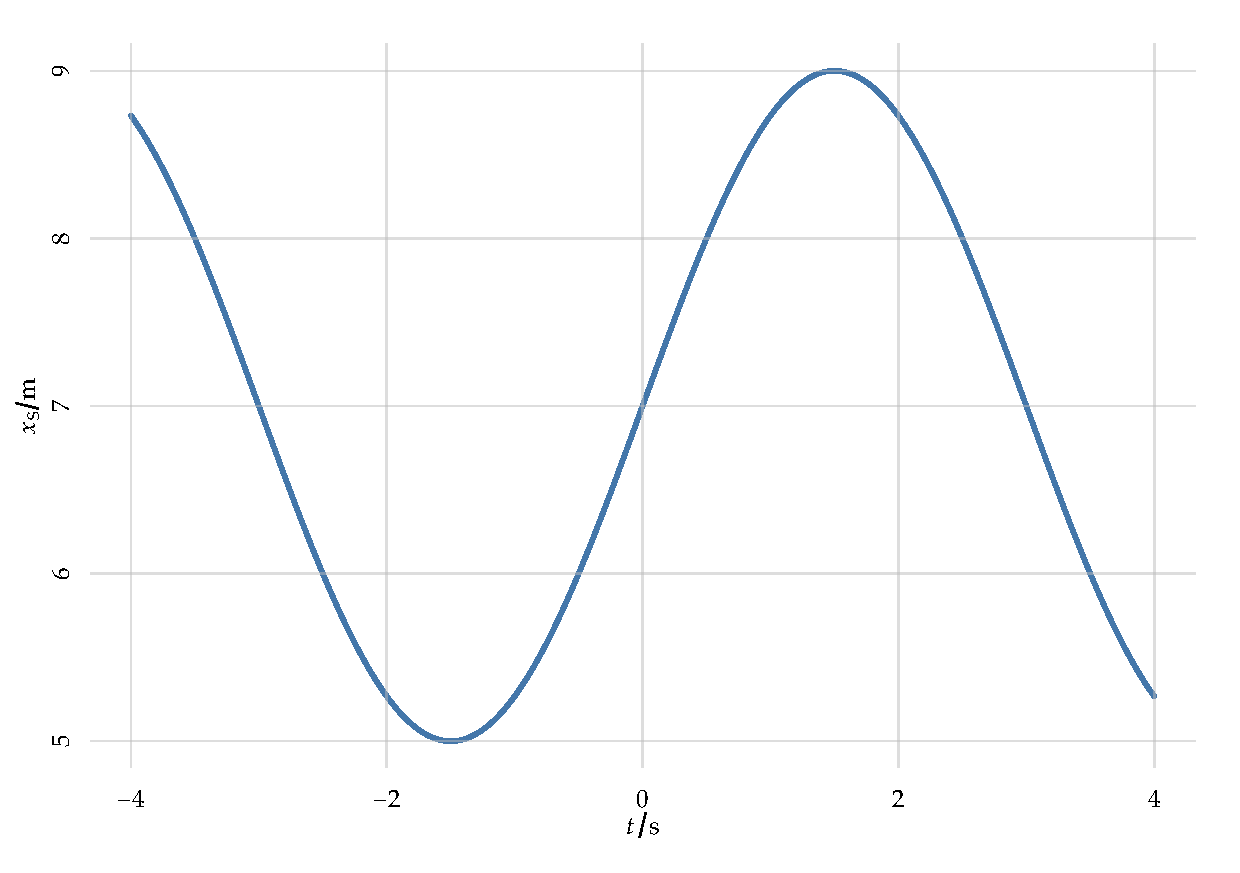
\includegraphics[width=0.49\linewidth]{images/xs.pdf}\hfill%
    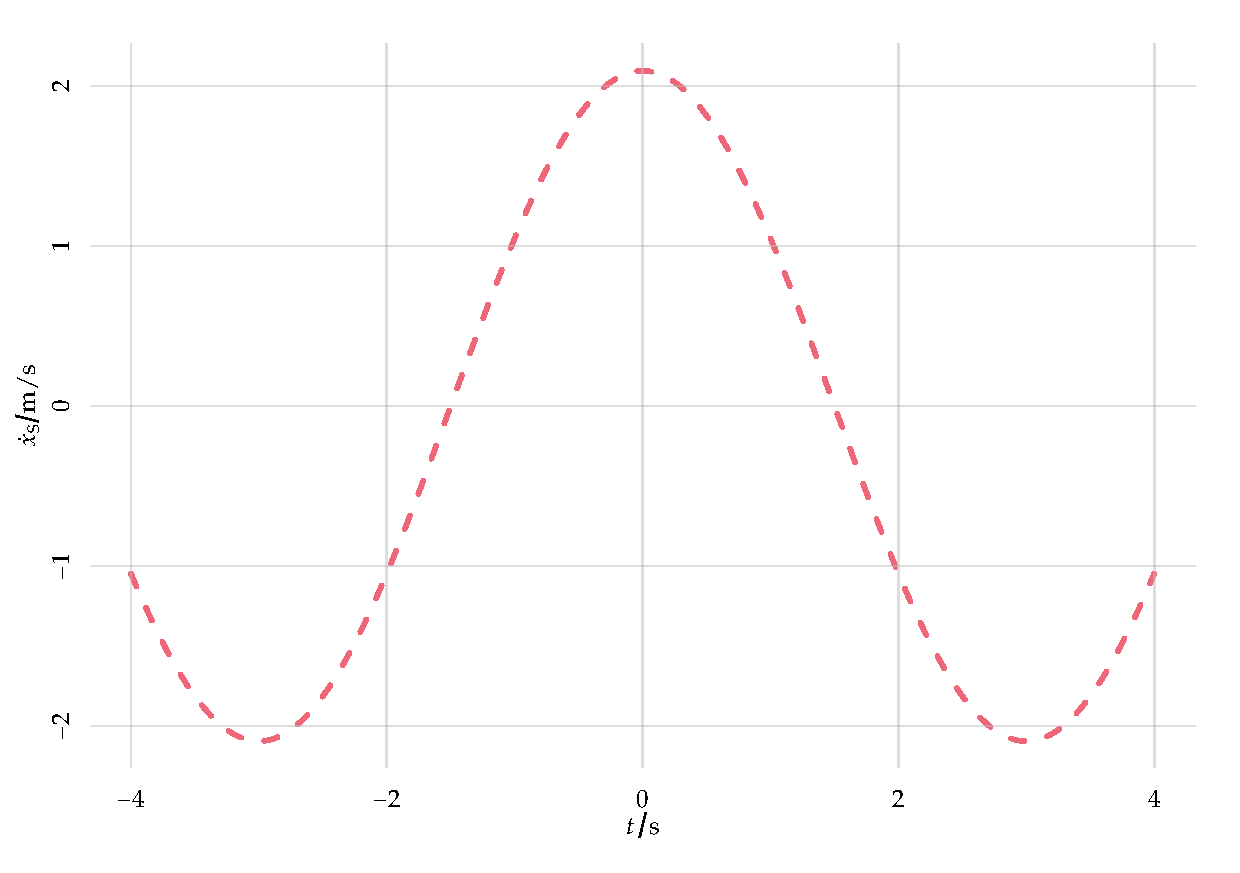
\includegraphics[width=0.49\linewidth]{images/vs.pdf}%
  \end{center}
  Or we could plot them on the same graph -- but only if we indicate separately the vertical axis for $\cx{S}$ and the one for $\vx{S}$ (for instance one on the left and one on the right), because these quantities have different dimensions.
\end{enumerate}


\sollabel{sec:3Dmotion_simple}

\begin{enumerate}[exerc]
\item No, the expression is not dimensionally correct, because the $z$ component of $\yr_{\text{S}}$ is \enquote{$0$}, which is a dimensionless number, whereas $z$ has dimension \textdim{length}. The $z$ component should be \enquote{\qty{0}{m}}.
\item See exercises~\ref{sec:1D_motion} and \ref{sec:1D_motion_b}\enskip\faIcon{smile}
\end{enumerate}

\sollabel{sec:1Dintegration}

\begin{enumerate}[exerc]
\item Let's call the specific position $z_{0} \defd \qty{-2}{m}$ at $\yti\qty{1}{s}$. The expression for $z(t)$ is found integrating $v_{z}(t)$ between $\yti$ and $t$, and adding the position at $\yti$:
  \begin{equation*}
    \begin{split}
      z(t) &= z_{0} + \int_{\yti}^{t} c \exp(-t/\tau) \dt
      \\[\jot]
      &= z_{0} - c \tau \exp(-t/\tau)\bigr\rvert_{\yti}^{t}
      \\[\jot]
      &= z_{0} - c \tau \bigl[\exp(-t/\tau) - \exp(-\yti/\tau)\bigr]
      \\[2\jot]
      &\qquad\text{with}\quad
  c = \qty{299792458}{m/s} \,,\
  \tau = \qty{0.08}{s} \,,\
  z_{0} = \qty{-2}{m}\,,\
  \yti = \qty{1}{s} \ .
    \end{split}
  \end{equation*}

\item Substituting in the expression above, $z(\qty{1.01}{s}) = \qty{8.50}{m}$\,.
\end{enumerate}


%% **** add exercise on Veritasium's \furl{https://www.youtube.com/watch?v=pTn6Ewhb27k}{\emph{Why No One Has Measured The Speed Of Light}}



% \section{Time and proper time}
% \label{sec:time}


% \section{Coordinate time}
% \label{sec:coord_time}


% \section{Space, length, distance}
% \label{sec:difficulties_distance}


% \section{Coordinate systems}
% \label{sec:coords}


% \section{Spatial coordinate distance and length}
% \label{sec:coord_distance}


% \section{Coordinate notation}
% \label{sec:coord_notation}


% \section{Velocity and acceleration}
% \label{sec:velocity}

\printpagenotes*
\cleartooddpage
\chapter{Main physical quantities}
\label{cha:stuff}
\setcounter{section}{-1}

\section{}
(Do the \textcolor{yellow}{exercises} in the main text.)



\section{}
\label{sec:extensive_vs_meas}

We have seen that six of the seven main physical quantities have two important properties:
\begin{itemize}[nosep]
\item We can speak about their \emph{content}, \emph{flux}, and \emph{supply}.
\item They are \emph{extensive}: for instance if a 3D region consists of two non-overlapping 3D subregions, then the content in the region is the sum of the content in the subregions. Similarly for flux and surfaces (2D regions).
\end{itemize}

\begin{enumerate}[exerc]
\item Can you think of some physical quantity that has the property of extensivity, but for which it doesn't make sense to speak of \enquote{content} or of \enquote{flux} or of \enquote{supply}?

\item Vice versa, can you think of some physical quantity for which we can speak of content, flux, supply, but which doesn't have the property of extensivity?
\end{enumerate}

\section{}
\label{sec:energy_meas_mass}

Do a little research, and find out whether there are any physics disciplines in which \emph{mass} is usually measured in units of \emph{energy}.

\section{}
\label{sec:energy_meas_mass}

Do a little research, and find out whether there are any physics disciplines in which \emph{mass} is usually measured in units of \emph{energy}.


\section{}
\label{sec:diff_mass_matter}

\emph{With a colleague or a large language model:}

\smallskip

Take turns to explain to each other what is the difference between \emph{matter} and \emph{mass}. Try to find weak points in each other's explanations.


\section{}
\label{sec:neg_matter}

\begin{enumerate}[exerc]
\item Imagine that someone tells you this:
  \begin{quote}
    An important difference between \emph{matter} and \emph{electric charge} is that electric charge can be both positive and negative, whereas matter can only be positive.
  \end{quote}
  How would you reply? Can you give counterexamples to this statement?

\item The same person tells you:
  \begin{quote}
    In nature we observe both positive and negative electric charge equally easily. But we mostly observe \enquote*{positive} matter, and very rarely \enquote*{negative} matter (antimatter).
  \end{quote}
  Do some research and find out whether this statement is true.
\end{enumerate}

\section{}
\label{sec:energy_vs_mass}

Someone tells you:
\begin{quote}
  \emph{Mass} and \emph{energy} are two different things. I can experimentally prove it to you: Take a battery for example, and weigh it to measure its mass. Now use the battery for some device. As you use it, the battery loses energy; in fact eventually it can't power the device anymore. But if you weigh it again, you'll find that it has the same mass as before. Therefore mass and energy must be two different things.
\end{quote}
How would you reply to this person?



\section{}
\label{sec:net_amount}

Let's say you use a coordinate system $(x,y,z)$. In a given 3D region of space you measure a net amount (content) of momentum $\yP = [2, -3, 0]\,\unit{N\,s}$. Which of the following statements are true? which false? Explain why.
\begin{enumerate}[exerc]
\item There must be some non-zero electric charge in the 3D region.
\item The net amount of momentum has zero $z$-component.
\item There must be some matter (or antimatter) in the 3D region.
\item The 3D region must be enough small.
\item Some kind of motion, with respect to your coordinate system, must be occurring in the 3D region.
\item Any scientist measuring the net momentum in the 3D region would agree that its value is $[2, -3, 0]\,\unit{N\,s}$.
\item Whatever it is that contributes to the net momentum, it must be uniformly spread out through the whole 3D region.
\end{enumerate}




\clearpage
\addsec{Example solutions}

\sollabel{sec:extensive_vs_meas}

\emph{[Before reading this answer, keep in mind that the word \emph{volume} has two different meanings: sometimes we use it in the sense of \enquote{3D region of space}; sometimes in the sense of the \emph{size} of a 3D region of space (measured in cubic metres for instance).]}

\begin{enumerate}[exerc]
\item One example is the \emph{volume} of a 3D region. It is extensive, because the volume of two non-overlapping 3D regions together is the sum of their volumes. But it doesn't make much sense to speak of the \enquote{flux} of volume through a surface. Similarly for \emph{area}.

\item The writer of this solution doesn't know any example of such a physical quantity. It is possible to define mathematical objects that behave this strange way, but no physical quantity seems to be represented by such objects.
\end{enumerate}


\sollabel{sec:energy_meas_mass}

One example is \furl{https://cms.cern/content/glossary\#E}{particle physics}, where the rest mass of subatomic particles is measured in \emph{electronvolts}, denoted \enquote*{\unit{eV}}, which is a unit for energy equal to \qty{1.602176634e-19}{J}. Other examples are special relativity and general relativity.



\sollabel{sec:net_amount}

\begin{enumerate}[exerc]
\item \emph{False.} There can be momentum in a region even if the net electric charge is zero.
\item \emph{True.} $z$ is the third coordinate, and the third momentum component is \qty{0}{N\,s}.
\item \emph{False.} Electromagnetic fields have momentum, so in the region there could be only an electromagnetic field, such as a beam of light, but no matter.
\item \emph{False.} We can speak of the net amount of momentum in arbitrarily large regions.
\item \emph{True.} Momentum is associated with the motion of matter or of electromagnetic fields.
\item \emph{False.} The amount of momentum depends on the coordinate system we choose; so  scientists that use coordinates different from yours will measure a different net momentum -- it could even be completely zero.
\item \emph{False.} The matter or electromagnetic field that possess the momentum might be concentrated in one or several small regions within the 3D region, for example.
\end{enumerate}


% \section{Matter}
% \label{sec:intro_matter}


% \section{Electric charge}
% \label{sec:intro_charge}


% \section{Magnetic flux}
% \label{sec:intro_magneticflux}


% \section{Energy-mass}
% \label{sec:intro_energy}


% \section{Momentum}
% \label{sec:intro_momentum}


% \section{Angular momentum}
% \label{sec:intro_angmomentum}


% \section{Entropy}
% \label{sec:intro_entropy}


% \section{Auxiliary quantities}
% \label{sec:aux_quantities}


% \section{Temperature}
% \label{sec:temperature}


% \section{Metric}
% \label{sec:metric}


\printpagenotes*
\cleartooddpage
\chapter{Volume contents, fluxes, supplies}
\label{cha:contents_fluxes}
\setcounter{section}{-1}

\section{}
(Do the \textcolor{yellow}{exercises} in the main text.)


\section{}
\label{sec:contents}

In the following figures, \textcolor{blue}{region A is indicated in blue and a solid contour}, and \textcolor{red}{region B is indicated in red and a dashed contour} (they are 2D simplified representations of 3D regions). For each figure determine, if possible, the net volume content of the corresponding quantities in the region comprising A and B. If not possible, explain why.

\begin{enumerate}[exerc,itemsep=2ex]
\item Energy-mass:\qquad 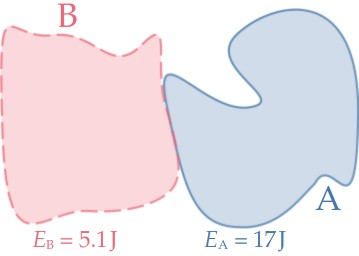
\includegraphics[align=c,height=10em]{images/ex_AB_J1.jpg}%
\item Matter:\qquad 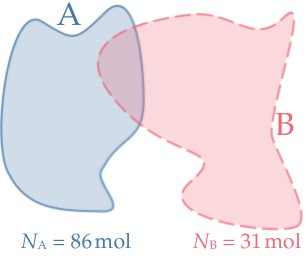
\includegraphics[align=c,height=10em]{images/ex_AB_mol1.jpg}%
\item Electric charge:\qquad 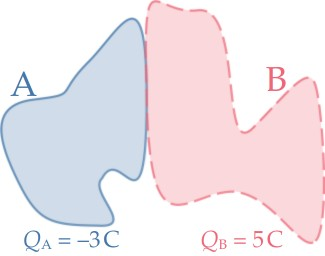
\includegraphics[align=c,height=10em]{images/ex_AB_C1.jpg}%
\item Energy-mass:\qquad 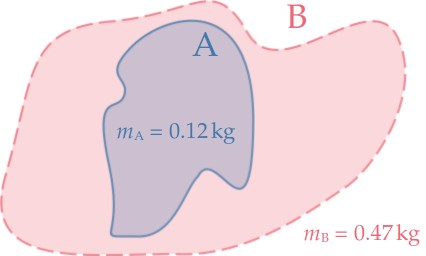
\includegraphics[align=c,height=10em]{images/ex_AB_kgin.jpg}%
\end{enumerate}


\section{}
\label{sec:Pcontents}

In the following figures, \textcolor{blue}{region A is indicated in blue and a solid contour}, and \textcolor{red}{region B is indicated in red and a dashed contour} (they are 2D simplified representations of 3D regions). Use a coordinate system $(x,y,z)$ where $x$ is horizontal to the right, $y$ is vertical upwards on the page, and $z$ comes out of the page towards you. For each figure:
\begin{itemize}[nosep]
\item draw the vectors representing the momentum contents of A and B;
\item determine, if possible, the net volume content of momentum in the region comprising A and B; if not possible, explain why.
\end{itemize}

\begin{enumerate}[exerc,itemsep=2ex]
\item \qquad 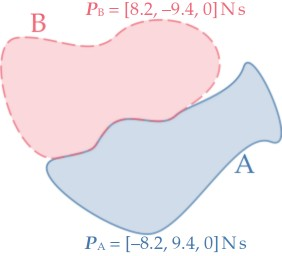
\includegraphics[align=c,height=11em]{images/ex_AB_P0.jpg}%
\item \qquad 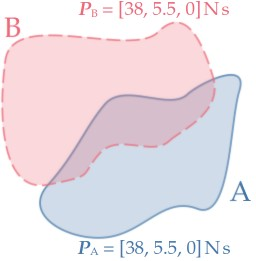
\includegraphics[align=c,height=11em]{images/ex_AB_Pov.jpg}%
\item \qquad 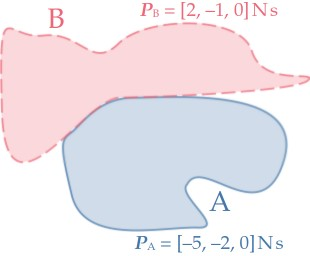
\includegraphics[align=c,height=11em]{images/ex_AB_P1.jpg}%
\item \qquad 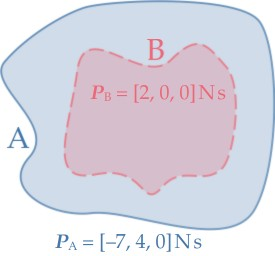
\includegraphics[align=c,height=11em]{images/ex_AB_Pin.jpg}%
\item \qquad 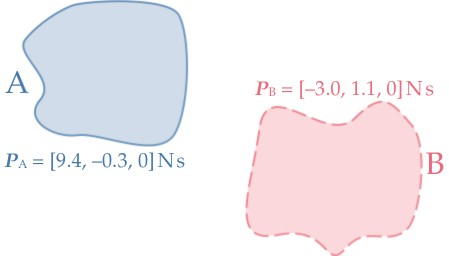
\includegraphics[align=c,height=11em]{images/ex_AB_Pdi.jpg}%
\end{enumerate}


\section{}
\label{sec:P_ball_light}

\marginpar{\vspace{0\baselineskip}\centering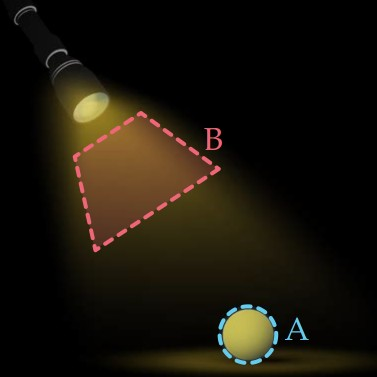
\includegraphics[width=\linewidth]{images/ex_AB_light_ball.jpg}%
}%
In the side figure, consider \textcolor{cyan}{volume~A}, which contains the ball, and \textcolor{red}{volume~B}, occupied by the light beam. Imagine there's no air (although in reality if there were no air we wouldn't be able to see the light beam).

In a given coordinate system, the momentum content of volume A is $\yP_{\text{A}} = [1, 0,0 ]\,\unit{N\,s}$, and that of volume B is $\yP_{\text{B}} = [2, -2, 1]\times\qty{e-16}{N\,s}$.

Does it really make sense to speak of the momentum in volume B (remember there's no air there)? If it does make sense, how much is the net momentum content of volumes A and B considered together?


\section{}
\label{sec:flux_sense}

\marginpar{\vspace{0\baselineskip}\centering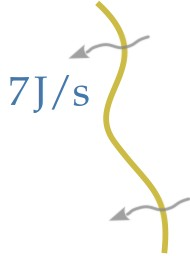
\includegraphics[height=7em]{images/Jflux_main.jpg}%
}%
Take a look at the energy flux through a surface represented in the side figure. Which of the representations below is completely equivalent to the one on the side? Which does represent a different flux instead?\noprelistbreak

\renewcommand{\tabularxcolumn}[1]{>{\bfseries}w{c}{0.3\linewidth}}
\begin{tabularx}{\linewidth}[h]{XXX}
1.&2.&3.
\\
  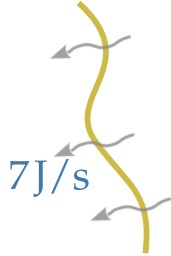
\includegraphics[align=c,height=6em]{images/Jflux_main1.jpg}
&  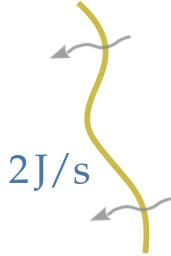
\includegraphics[align=c,height=6em]{images/Jflux_main2.jpg}
&  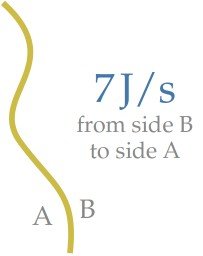
\includegraphics[align=c,height=6em]{images/Jflux_main3.jpg}
\\[10ex]
4.&5.&6.
\\
  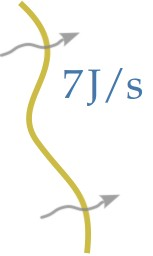
\includegraphics[align=c, height=6em]{images/Jflux_main5.jpg}
&  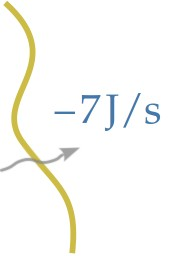
\includegraphics[align=c, height=6em]{images/Jflux_main6.jpg}
&  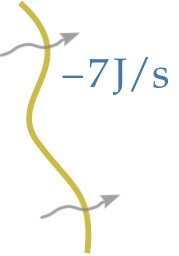
\includegraphics[align=c, height=6em]{images/Jflux_main7.jpg}
\end{tabularx}


\section{}
\label{sec:battery_wire}

\marginpar{\vspace{0\baselineskip}\centering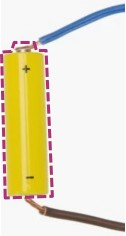
\includegraphics[height=7\baselineskip]{images/battery_wire_CS.jpg}%
}%
An ordinary battery is attached to wires and is powering some device. This means that there is a flow of electromagnetic energy from the battery to the device. Imagine a control surface around the battery, as illustrated in the side figure. Can you guess across which parts of the control surface is the flux of energy? Is it across the whole surface? or only across the parts where the wire is? Do a little research to find out.

\section{}
\label{sec:sum_fluxes}

A cuboid region is delimited by a closed control surface that can be divided into six parts; call them \enquote*{up}, \enquote*{down}, \enquote*{front}, \enquote*{back}, \enquote*{left}, \enquote*{right}. They are all have an inward crossing direction, except for \enquote*{back} which has an outward crossing direction.

Here are the fluxes of various quantities through the six surfaces in the given crossing directions. Calculate the total net \textbf{in}fluxes.\noprelistbreak

\smallskip

\begin{enumerate}[exerc,itemsep=1em]
\item
  $
  \begin{aligned}[t]
    \yJ_{\text{u}} &= \qty{23.9}{mol/s}&\quad
    \yJ_{\text{d}} &= \qty{-8.1}{mol/s}&\quad
    \yJ_{\text{f}} &= \qty{0.9}{mol/s}\\
    \yJ_{\text{b}} &= \qty{-30.5}{mol/s}&\quad
    \yJ_{\text{l}} &= \qty{2.3}{mol/s}&\quad
    \yJ_{\text{r}} &= \qty{37.6}{mol/s}
  \end{aligned}
  $

\item
  $\begin{aligned}[t]
    \yH_{\text{u}} &= \qty{-24.6}{J/s} &\quad
    \yH_{\text{d}} &= \qty{2.4}{J/s} &\quad
    \yH_{\text{f}} &= \qty{1.3}{J/s} \\
    \yH_{\text{b}} &= \qty{10.8}{J/s} &\quad
    \yH_{\text{l}} &= \qty{15.4}{J/s} &\quad
    \yH_{\text{r}} &= \qty{-2.1}{J/s}
  \end{aligned}$

\item
  $
  \begin{aligned}[t]
    \yI_{\text{u}} &= \qty{-9.7}{C/s} &\quad
    \yI_{\text{d}} &= \qty{27.4}{C/s} &\quad
    \yI_{\text{f}} &= \qty{-6.3}{C/s} \\
    \yI_{\text{b}} &= \qty{16.4}{C/s} &\quad
    \yI_{\text{l}} &= \qty{-25.1}{C/s} &\quad
    \yI_{\text{r}} &= \qty{-20.0}{C/s} 
  \end{aligned}
  $

\item
  $
  \begin{aligned}[t]
    \yB_{\text{u}} &= \qty{31.7}{J/(K\,s)} &\quad
    \yB_{\text{d}} &= \qty{17.9}{J/(K\,s)} &\quad
    \yB_{\text{f}} &= \qty{7.2}{J/(K\,s)} \\
    \yB_{\text{b}} &= \qty{-20.4}{J/(K\,s)} &\quad
    \yB_{\text{l}} &= \qty{-16.5}{J/(K\,s)} &\quad
    \yB_{\text{r}} &= \qty{-4.8}{J/(K\,s)}
  \end{aligned}
  $

\item
  $
  \begin{aligned}[t]
    \yF_{\text{u}} &= [25.2, -42.7, 4.1]\,\unit{N} &\quad
    \yF_{\text{d}} &= [-46.3, -5.9, -33.3]\,\unit{N} \\
    \yF_{\text{f}} &= [10.2, -16.2, -36.7]\,\unit{N} &\quad
    \yF_{\text{b}} &= [-9.8, 19.5, -60.0]\,\unit{N} \\ 
    \yF_{\text{l}} &= [29.5, 18.3, 58.4]\,\unit{N} &\quad
    \yF_{\text{r}} &= [16.0, 1.2, -3.2]\,\unit{N}
  \end{aligned}
  $
\end{enumerate}



\section{}
\label{sec:fluxes_scalar}

\renewcommand{\tabularxcolumn}[1]{>{\bfseries}w{c}{0.3\linewidth}}
Which of the following graphical representations of fluxes do make sense? Which don't? Explain why.\noprelistbreak

\begin{tabularx}{\linewidth}[h]{XXX}
1.&2.&3.
\\
  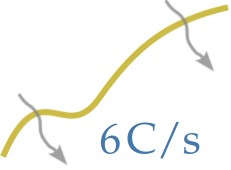
\includegraphics[align=c, height=6em,width=0.25\linewidth,keepaspectratio]{images/flux_scalar_1.jpg}
&  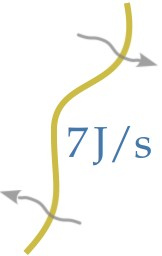
\includegraphics[align=c, height=6em,width=0.25\linewidth,keepaspectratio]{images/flux_scalar_2.jpg}
&  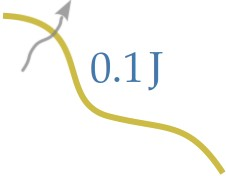
\includegraphics[align=c,height=6em,width=0.25\linewidth,keepaspectratio]{images/flux_scalar_4.jpg}
\\[10ex]
4.&5.&6.
\\
  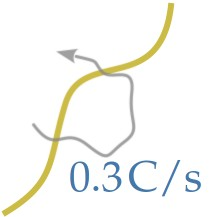
\includegraphics[align=c, height=6em,width=0.25\linewidth,keepaspectratio]{images/flux_scalar_5.jpg}
&  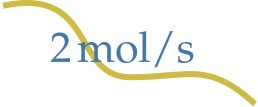
\includegraphics[align=c, height=6em,width=0.25\linewidth,keepaspectratio]{images/flux_scalar_6.jpg}
&  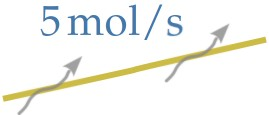
\includegraphics[align=c, height=6em,width=0.25\linewidth,keepaspectratio]{images/flux_scalar_7.jpg}
\\[10ex]
7.&8.&9.
\\
  
\includegraphics[align=c, height=6em,width=0.25\linewidth,keepaspectratio]{images/flux_scalar_8.jpg}
&  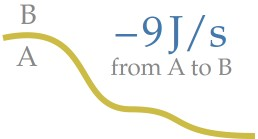
\includegraphics[align=c, height=6em,width=0.25\linewidth,keepaspectratio]{images/flux_scalar_9.jpg}
&  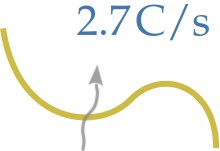
\includegraphics[align=c, height=6em,width=0.25\linewidth,keepaspectratio]{images/flux_scalar_10.jpg}
\end{tabularx}

\medskip

\section{}
\label{sec:surface_moves_if_flux}

\begin{enumerate}[exerc]
\item A control volume contains $[2,-3,1]\,\unit{N\,s}$ of momentum. Momentum is a quantity related to movement. Does this mean that the control volume is moving?
\item Suppose that through a control surface, in a given crossing direction, there is a non-zero flux of momentum. Does this mean that the control surface must be in motion?
\item If through a control surface there's a non-zero flux of some quantity, does it mean that the fluxes of all other quantities must be zero?

\item Can there be a flux of temperature through a control surface?
\end{enumerate}

\section{}
\label{sec:fluxes_vector}

Which of the following graphical representations of fluxes do make sense? Which don't? Explain why.\noprelistbreak

\renewcommand{\tabularxcolumn}[1]{>{\bfseries}w{c}{0.3\linewidth}}
\begin{tabularx}{\linewidth}[h]{XXX}
1.&2.&3.
\\
  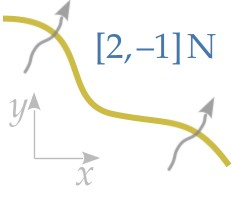
\includegraphics[align=c, height=6em,width=0.25\linewidth,keepaspectratio]{images/flux_vector_1.jpg}
&  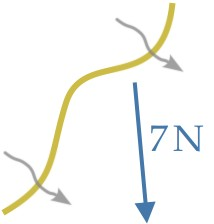
\includegraphics[align=c, height=6em,width=0.25\linewidth,keepaspectratio]{images/flux_vector_2.jpg}
&  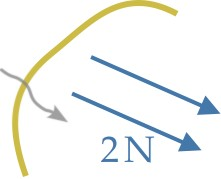
\includegraphics[align=c,
height=6em,width=0.25\linewidth,keepaspectratio]{images/flux_vector_3.jpg}
\\[10ex]
4.&5.&6.
\\
  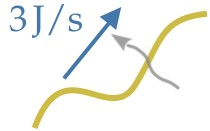
\includegraphics[align=c, height=6em,width=0.25\linewidth,keepaspectratio]{images/flux_vector_4.jpg}
&  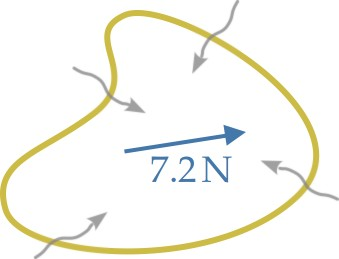
\includegraphics[align=c, height=6em,width=0.25\linewidth,keepaspectratio]{images/flux_vector_5.jpg}
&  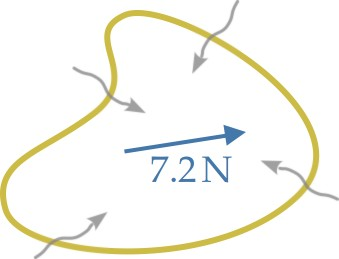
\includegraphics[align=c, height=6em,width=0.25\linewidth,keepaspectratio]{images/flux_vector_8.jpg}
\\[10ex]
7.&8.&9.
\\
  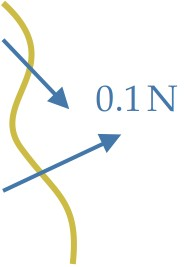
\includegraphics[align=c, height=6em,width=0.25\linewidth,keepaspectratio]{images/flux_vector_7.jpg}
&  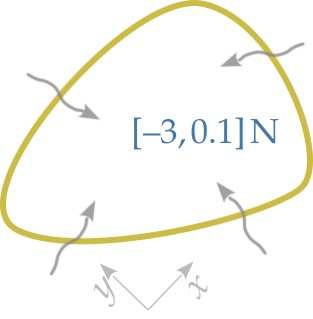
\includegraphics[align=c, height=6em,width=0.25\linewidth,keepaspectratio]{images/flux_vector_6.jpg}
&  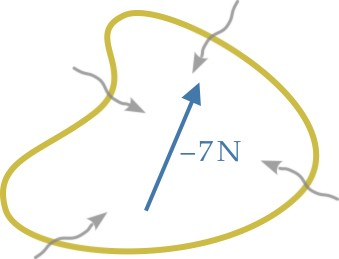
\includegraphics[align=c, height=6em,width=0.25\linewidth,keepaspectratio]{images/flux_vector_9.jpg}
\end{tabularx}


\section{}
\label{sec:moebius}

\marginpar{\vspace{0\baselineskip}\centering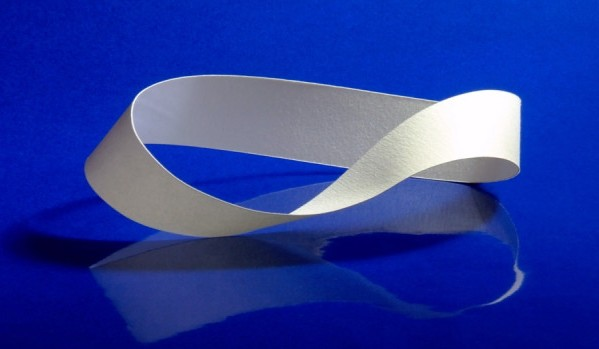
\includegraphics[width=\linewidth]{images/moebius_band.jpg}%
}%
The \furl{https://mathworld.wolfram.com/MoebiusStrip.html}{Möbius band} is a surface that, in a certain sense, has only \emph{one} side. It is quite easy to make with a strip of paper and some tape.

Do you manage to choose a definite crossing direction on this surface? Do you think it could be chosen as a control surface?


\section{}
\label{sec:netflux}

For each figure, calculate and draw, or describe precisely, the net total flux through the composite control surface. (The different parts are differentiated by different colours and thicknesses.) Don't forget to specify the crossing direction when you speak about a flux.\noprelistbreak

\renewcommand{\tabularxcolumn}[1]{>{\bfseries}w{c}{0.45\linewidth}}
\begin{tabularx}{\linewidth}[h]{XX}
1.&2.
\\
  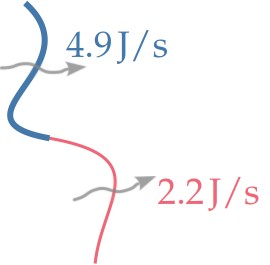
\includegraphics[align=c, height=9em,width=0.4\linewidth,keepaspectratio]{images/sumJ.jpg}
&  \includegraphics[align=c, height=9em,width=0.4\linewidth,keepaspectratio]{images/summol.jpg}
\\[15ex]
3.&4.
\\
 \includegraphics[align=c,
height=9em,width=0.4\linewidth,keepaspectratio]{images/sumC.jpg}
&  \includegraphics[align=c, height=9em,width=0.4\linewidth,keepaspectratio]{images/sumN1.jpg}
\\[15ex]
5.&6.
\\
 \includegraphics[align=c, height=9em,width=0.4\linewidth,keepaspectratio]{images/sumN2.jpg}
&  \includegraphics[align=c, height=9em,width=0.4\linewidth,keepaspectratio]{images/sumN3.jpg}
\end{tabularx}


\section{}
\label{sec:integrated_flux}

\begin{enumerate}[exerc]
\item Through a particular closed control surface there's a continuous influx of electric charge $\yI(t)$ with the following time dependence:
  \begin{equation*}
    \yI(t) = A \sin(\omega t) \qquad
    \text{with}\quad  A = \qty{30}{C/s}\ ,\quad \omega = \qty{376.991184}{s^{-1}} \ .
  \end{equation*}

  How much is the time-integrated influx of charge between times $\yti = \qty{10}{s}$ and $\ytf = \qty{40}{s}$?

\item Imagine a closed control surface around the planet Mercury. The energy $\yH(t)$ influx through this control surface is approximately given by
  \begin{multline*}
    \yH(t) = W + u\, \cos(\sigma t) \\
    \text{with}\quad  W = \qty{2e17}{J/s}\ ,\quad
    u = \qty{8e16}{J/s}\ ,\quad
    \sigma = \qty{8e-7}{s^{-1}} \ .
  \end{multline*}

  Mercury's year lasts around 88 Earth-days. How much is the time-integrated influx of energy over a year on Mercury?

\item A football has a \masse\ $\ym = \qty{0.4}{kg}$. The football has a continuous supply of momentum $\yG(t)$ from the Earth's gravitational field. This supply is constant in time and given by
  \begin{equation*}
    \yG(t) = \ym \yg
    \begin{bmatrix}
      0\\0\\-1
    \end{bmatrix}
  \end{equation*}
  where $\yg = \qty{9.8}{N/kg}$, and we are using a coordinate system $(t,x,y,z)$ where $z$ is vertical with respect to the ground and points upwards.

    How much is the time-integrated influx of momentum in the football between times $\yti = \qty{0}{s}$ and $\ytf = \qty{3600}{s}$?
\end{enumerate}

\clearpage
\addsec{Example solutions}

\sollabel{sec:contents}

\begin{enumerate}[exerc]
\item Net \energym\ content is $\yE_{\text{A}} + \yE_{\text{B}} = \qty{22.1}{J}$.
\item Unknown: A and B are overlapping, so we cannot simply add their contents. The result depends on the net matter content in the overlap region, which is unknown.
\item Net electric-charge content is $\yC_{\text{A}} + \yC_{\text{B}} = \qty{2}{C}$.
\item A and B are overlapping, so we cannot simply add their \masse\ contents. But in this case A is a subregion of B, so the full region occupied by both is B itself. The net \masse\ content in this region is therefore $\ym_{\text{B}} = \qty{0.47}{kg}$. We can also deduce that the net \masse\ content in the region between A and B is $\ym_{\text{B}} - \ym_{\text{A}} = \qty{0.35}{kg}$.
\end{enumerate}


\sollabel{sec:Pcontents}
\begin{enumerate}[exerc]
\item Net momentum content is $\yP_{\text{A}} + \yP_{\text{B}} = [0,0,0]\,\unit{N\,s}$.
\item Unknown: A and B are overlapping, so we cannot simply add their momentum contents. The result depends on the net momentum content in the overlap region, which is unknown.
\item Net momentum content is $\yP_{\text{A}} + \yP_{\text{B}} = [-3,-3,0]\,\unit{N\,s}$.
\item A and B are overlapping, so we cannot simply add their momentum contents. But in this case B is a subregion of A, so the full region occupied by both is A itself. The net momentum content in this region is therefore $\yP_{\text{A}} = [-7,4,0]\,\unit{N\,s}$. We can also deduce that the net momentum content in the region between B and A is  $\yP_{\text{A}} - \yP_{\text{B}} = [-9,4,0]\,\unit{N\,s}$.
\item Net momentum content is $\yP_{\text{A}} + \yP_{\text{B}} = [6.4,0.8,0]\,\unit{N\,s}$. The region consisting of A and B together is a spatially disconnected region, but we can speak of volume content even for such kind of regions.
\end{enumerate}


\sollabel{sec:P_ball_light}

Yes, it does make sense. First of all, we can \emph{always} speak of the momentum content in \emph{any} 3D region; it isn't important whether there's matter or electromagnetic fields or not in that region. If it's completely empty, its momentum content is simply zero. Second, in volume B in the figure there's an electromagnetic field, which does have momentum just like matter.

The net momentum content in the volumes A and B considered together is $\yP_{\text{A}} + \yP_{\text{B}} \approx [1, \qty{-2e-16}, \qty{1e-16}]\,\unit{N\,s}$.



\sollabel{sec:flux_sense}

\renewcommand{\tabularxcolumn}[1]{>{\bfseries}w{c}{0.3\linewidth}}
\begin{tabularx}{\linewidth}[h]{XXX}
1.&2.&3.
\\
Same \faIcon{thumbs-up}
&\textcolor{red}{Different \faIcon{thumbs-down}}
&Same \faIcon{thumbs-up}
\\
\parbox[t]{0.25\linewidth}{\normalfont\raggedright Same crossing direction, same flux magnitude. Wiggly arrows only indicate the crossing direction, it doesn't matter how many there are.}
&\parbox[t]{0.25\linewidth}{\normalfont\raggedright This flux has a different magnitude.}
&\parbox[t]{0.25\linewidth}{\normalfont\raggedright Same crossing direction, same flux magnitude. Crossing direction is indicated verbally.}
\\[15ex]
4.&5.&6.
\\
\textcolor{red}{Different \faIcon{thumbs-down}}
&Same \faIcon{thumbs-up}
&Same \faIcon{thumbs-up}
\\
\parbox[t]{0.25\linewidth}{\normalfont\raggedright This flux has same magnitude but opposite direction.}
&\parbox[t]{0.25\linewidth}{\normalfont\raggedright Same flux, by the principle of symmetry of flux.}
&\parbox[t]{0.25\linewidth}{\normalfont\raggedright Same flux, by the principle of symmetry of flux.}
\end{tabularx}


\sollabel{sec:battery_wire}

\marginpar{\vspace{0\baselineskip}\centering\includegraphics[height=7\baselineskip]{images/battery_wire_CS.jpg}%
}%
The flux of electromagnetic energy occurs -- that is, it is non-zero -- across \emph{every part of the control surface}, not just across the parts close to the wire.

In general the flow of electromagnetic energy occurs especially around wires, which act as sort of guides; but it extends to all space.

Two good videos for learning more about this are \emph{Veritasium}'s \furl{https://www.youtube.com/watch?v=bHIhgxav9LY}{\emph{The big misconception about electricity}} and \furl{https://www.youtube.com/watch?v=oI_X2cMHNe0}{\emph{How electricity actually works}}. More detailed examples, calculations, and figures can be found for example in \cites{jackson1996} (see especially \fig~4), \cites{davisetal2011},  \cites{harbola2010}, \cites{boyer2019b}.



\sollabel{sec:sum_fluxes}

To calculate the efflux across the whole surface we use the principle of extensivity. The fluxes across the \enquote*{back} surface get a minus sign, because that surface had an inward crossing direction.
\begin{enumerate}[exerc]
\item $\yJ_{\text{tot}} =
  \yJ_{\text{u}} + \yJ_{\text{d}} + \yJ_{\text{f}}
  - \yJ_{\text{b}} + \yJ_{\text{l}} + \yJ_{\text{r}} =
 \qty{87.1}{mol/s}$

\item $\yH_{\text{tot}} =
  \yH_{\text{u}} + \yH_{\text{d}} + \yH_{\text{f}}
  - \yH_{\text{b}} + \yH_{\text{l}} + \yH_{\text{r}} =
 \qty{-18.4}{J/s}$

\item $\yI_{\text{tot}} =
  \yI_{\text{u}} + \yI_{\text{d}} + \yI_{\text{f}}
  - \yI_{\text{b}} + \yI_{\text{l}} + \yI_{\text{r}} =
 \qty{-50.1}{C/s}$

\item $\yB_{\text{tot}} =
  \yB_{\text{u}} + \yB_{\text{d}} + \yB_{\text{f}}
  - \yB_{\text{b}} + \yB_{\text{l}} + \yB_{\text{r}} =
 \qty{-50.1}{C/s}$

\item $\yF_{\text{tot}} =
  \yF_{\text{u}} + \yF_{\text{d}} + \yF_{\text{f}}
  - \yF_{\text{b}} + \yF_{\text{l}} + \yF_{\text{r}} =
 [44.4, -64.8, 49.3]\,\unit{C/s}$

\end{enumerate}

\sollabel{sec:fluxes_scalar}

\renewcommand{\tabularxcolumn}[1]{>{\bfseries}w{c}{0.3\linewidth}}
\begin{tabularx}{\linewidth}[h]{XXX}
1.&2.&3.
\\
Makes sense \faIcon{thumbs-up}
&\textcolor{red}{No \faIcon{thumbs-down}}
&\textcolor{red}{No \faIcon{thumbs-down}}
\\
&\parbox[t]{0.25\linewidth}{\normalfont\raggedright Crossing direction is unclear.}
&\parbox[t]{0.25\linewidth}{\normalfont\raggedright \enquote*{\unit{J}} is not the unit of a flux.}
\\[5ex]
4.&5.&6.
\\
\textcolor{red}{No \faIcon{thumbs-down}}
&\textcolor{red}{No \faIcon{thumbs-down}}
&Makes sense \faIcon{thumbs-up}
\\
\parbox[t]{0.25\linewidth}{\normalfont\raggedright Crossing direction is unclear.}
&\parbox[t]{0.25\linewidth}{\normalfont\raggedright Crossing direction is missing.}
&\parbox[t]{0.25\linewidth}{\normalfont\raggedright The arrows for the crossing direction are very tilted, but crossing direction is still clear.}
\\[13ex]
7.&8.&9.
\\
\textcolor{red}{No \faIcon{thumbs-down}}
&Makes sense \faIcon{thumbs-up}
&Makes sense \faIcon{thumbs-up}
\\
\parbox[t]{0.25\linewidth}{\normalfont\raggedright \enquote*{\unit{N}} is the unit of a \textbf{vector} flux, but there's no vector or vector components here.}
&\parbox[t]{0.25\linewidth}{\normalfont\raggedright Alternative way of indicating the crossing direction, but perfectly clear.}
&
\end{tabularx}


\sollabel{sec:surface_moves_if_flux}

\begin{enumerate}[exerc]
\item No. If a control volume contains momentum, then something like matter or electromagnetic field is moving within the volume; but the volume itself may be static. This is because a control volume is just an imaginary delimitation of a region of space, not a physical object; we decide how it moves. In some situations we may decide that it should move together with the matter or electromagnetic field it contains, but in other situations we may keep it static.

\item No, for analogous reasons as in the answer above.

\item No: \emph{in principle} the fluxes of the seven quantities are independent and can all be non-zero; or some can be zero and others non-zero.

\item No: we can speak of the temperature at a point at a given time, but we cannot speak of volume content or flux or supply of temperature. Temperature is not an extensive quantity.
\end{enumerate}


\sollabel{sec:fluxes_vector}

\renewcommand{\tabularxcolumn}[1]{>{\bfseries}w{c}{0.3\linewidth}}
\begin{tabularx}{\linewidth}[h]{XXX}
1.&2.&3.
\\
Makes sense \faIcon{thumbs-up}
&Makes sense \faIcon{thumbs-up}
&\textcolor{red}{No \faIcon{thumbs-down}}
\\
\parbox[t]{0.25\linewidth}{\normalfont\raggedright This vector flux is expressed in components, and the coordinates are shown: we can reconstruct the vector if needed.}
&
&\parbox[t]{0.25\linewidth}{\normalfont\raggedright There should be only one vector indicating the flux. Unclear if this flux should have magnitude \qty{4}{N}.}
\\[20ex]
4.&5.&6.
\\
\textcolor{red}{No \faIcon{thumbs-down}}
&Makes sense \faIcon{thumbs-up}
&\textcolor{red}{No \faIcon{thumbs-down}}
\\
\parbox[t]{0.25\linewidth}{\normalfont\raggedright \enquote*{\unit{J/s}} is the unit of a \textbf{scalar} flux, but there's a vector here. Either the unit is wrong or the vector is there by mistake.}
&\parbox[t]{0.25\linewidth}{\normalfont\raggedright This is a total influx.}
&\parbox[t]{0.25\linewidth}{\normalfont\raggedright The wiggly arrows that indicate the crossing direction are not mutually consistent.}
\\[20ex]
7.&8.&9.
\\
\textcolor{red}{No \faIcon{thumbs-down}}
&Makes sense \faIcon{thumbs-up}
&\textcolor{red}{No \faIcon{thumbs-down}}
\\
\parbox[t]{0.25\linewidth}{\normalfont\raggedright Unclear if one of the two arrows indicates a crossing direction.}
&\parbox[t]{0.25\linewidth}{\normalfont\raggedright Total influx again. The flux is expressed in components, and the coordinates are shown.}
&\parbox[t]{0.25\linewidth}{\normalfont\raggedright The magnitude of a vector cannot be negative.}
\end{tabularx}


\sollabel{sec:moebius}

You have noticed that if you try to choose consistently a crossing direction on the whole band, you end up where you started but with an \emph{opposite} crossing direction. For this reason the Möbius band cannot be used as a control surface: it cannot be given an overall crossing direction. The lack of crossing direction is related to another peculiarity: it is impossible to extend this surface in such a way as to enclose a three-dimensional region of space.

If we clip a part of the Möbius band, that part can be used as a control surface. Or if we clip the band so that it gets an extra border, then it becomes the same as a twisted rectangle, and so it can be used as a control surface.


\sollabel{sec:netflux}

\renewcommand{\tabularxcolumn}[1]{>{\bfseries}w{c}{0.45\linewidth}}
\begin{tabularx}{\linewidth}[h]{XX}
1.&2.
\\
  \includegraphics[align=c, height=9em,width=0.4\linewidth,keepaspectratio]{images/sol_sumJ.jpg}
&  \includegraphics[align=c, height=9em,width=0.4\linewidth,keepaspectratio]{images/sol_summol.jpg}
\\[15ex]
3.&4.
\\
 \includegraphics[align=c,
height=9em,width=0.4\linewidth,keepaspectratio]{images/sol_sumC.jpg}
&  \includegraphics[align=c, height=9em,width=0.4\linewidth,keepaspectratio]{images/sol_sumN1.jpg}
\\[15ex]
5.&6.
\\
 \includegraphics[align=c, height=9em,width=0.4\linewidth,keepaspectratio]{images/sol_sumN2.jpg}
&  \includegraphics[align=c, height=9em,width=0.4\linewidth,keepaspectratio]{images/sol_sumN3.jpg}
\end{tabularx}


\sollabel{sec:integrated_flux}

\begin{enumerate}[exerc]
\item The time-integrated flux of charge is found with a time integral. Note that the result has a dimension of electric charge: this is the net amount of charge that flowed through the control surface, in the given crossing direction, between the two times:
  \begin{equation*}
    \begin{aligned}
      \int_{\yti}^{\ytf}\yI(t)\dt =
      \int_{\yti}^{\ytf}A \sin(\omega t)\dt
      &=
      -\frac{A}{\omega}\, \cos(\omega t)\Bigr\rvert_{\yti}^{\ytf}
      \\&\approx -\qty{796}{C}\cdot (1-1) = \qty{0}{C} \ .
    \end{aligned}
  \end{equation*}
  So even if the flux of charge most of the time is non-zero, reaching a maximum of $\pm\qty{30}{C/s}$, the \emph{net} amount of charge crossing the surface in the given direction during the \qty{30}{s} is zero. This is because the flux is sometimes positive, sometimes negative.

\item 88 Earth-days are approximately equal to $88\cdot 24\cdot 60\cdot \qty{60}{s} \approx \qty{7600000}{s}$. So we time-integrate between $\yti=\qty{0}{s}$ and $\ytf=\qty{7600000}{s}$:
  \begin{equation*}
    \begin{aligned}
      \int_{\yti}^{\ytf}\yH(t)\dt =
      \int_{\yti}^{\ytf}\bigl[W + u\, \cos(\sigma t)\bigr]\dt &=
      W t\Bigr\rvert_{\yti}^{\ytf} +
      \frac{u}{\sigma}\, \sin(\sigma t)\Bigr\rvert_{\yti}^{\ytf}
      \\[1ex]
      &\approx \qty{1.5e24}{J} +
      \qty{1e23}{J}\cdot (-0.2 - 0)
      \\&\approx \qty{1.5e24}{J} \ .
    \end{aligned}
  \end{equation*}

\item Recall that time-integrating a vector simply means time-integrating each component. In this case the supply is constant, so integration is easy:
  \begin{equation*}
    \begin{aligned}
      \int_{\yti}^{\ytf} \yG(t)\dt &=
      \int_{\yti}^{\ytf} \ym \yg
    \begin{bmatrix}
      0\\0\\-1
    \end{bmatrix}\dt
    \\[1ex]
    &= \ym \yg
    \begin{bmatrix}
      \int_{\yti}^{\ytf}0\dt\\[2\jot]
      \int_{\yti}^{\ytf}0\dt\\[2\jot]
      -\int_{\yti}^{\ytf}1\dt
    \end{bmatrix} =
      \ym \yg
    \begin{bmatrix}
      \qty{0}{s}\\\qty{0}{s}\\-t
    \end{bmatrix}\Biggr\rvert_{\yti}^{\ytf}
    =\ym \yg \left(
\begin{bmatrix}
      \qty{0}{s}\\\qty{0}{s}\\-\ytf
    \end{bmatrix}
    -
    \begin{bmatrix}
      \qty{0}{s}\\\qty{0}{s}\\-\yti
    \end{bmatrix}
    \right)
    \\[1ex]
    &\approx \qty{3.9}{N}\cdot
    \begin{bmatrix}
      0\\0\\-\num{3600}
    \end{bmatrix}\,\unit{s}
\approx
    \begin{bmatrix}
      0\\0\\-\num{1.4e4}
    \end{bmatrix}\,\unit{N\,s} \ .
    \end{aligned}
  \end{equation*}
  This net amount of momentum is vertical, pointing downward. But note that we don't know whether the football contains this much momentum after \qty{3600}{s}, because we don't know how much the flux of momentum into the football was. It's possible that the flux of momentum completely balanced this supply of momentum.
\end{enumerate}


% \section{Content in a volume and flux through a surface}
% \label{sec:contentflux}


% \section{Supply in a volume}
% \label{sec:supply}


% \section{Control volumes and control surfaces}
% \label{sec_controlvolumes_surfaces}


% \section{Volume content}
% \label{sec:intuition_volume}


% \section{Flux: scalar quantities}
% \label{sec:intuition_fluxes_scalar}


% \section{Flux: vector quantities}
% \label{sec:intuition_fluxes_vector}


% \section{Flux of momentum: force}
% \label{sec:force_is_flux}


% \section{Pressure, tension, shear force}
% \label{sec:pressure_tension_shear}


% \section{Closed control surfaces, influxes, effluxes}
% \label{sec:in_out_flux}


% \section{Time-integrated fluxes}
% \label{sec:total_flow}


% \section{Fluxes and velocities}
% \label{sec:fluxes_velocities}


% \section{Symbols for volume contents and fluxes}
% \label{sec:symbols_volint_flux}


\printpagenotes*
\cleartooddpage
\chapter{Physical laws}
\label{cha:laws}
\setcounter{section}{-1}

\section{}
(Do the \textcolor{yellow}{exercises} in the main text.)


% \section{}
% \label{sec:conservation_onlyalways}
% %% Observed conserved only in an instance: does it obey conservation law?

\section{}
\label{sec:calc_from_bal}

For each question:
\begin{itemize}[nosep,label=\faIcon{hand-point-right}]
\item Identify and describe the closed control surface and control volume used.
\item Identify which among volume content, flux, supply, are given, and how much they are; identify which are unknown.
\item Find the requested quantity, if possible, by using a balance or conservation law as specified in the question, showing all mathematical steps. If not possible, explain why.
\end{itemize}

\begin{enumerate}[exerc]
\item At a time of \qty{0}{s}, a tank contains \qty{10}{mol} of water, plus other substances. The tank is sealed. In a time lapse of \qty{20}{s} an amount of \qty{3}{mol} of water is produced in the tank by chemical reaction. Assume that the amount of water satisfies a balance law. How much water is in the tank at the end of this time lapse?

\item In \qty{30}{min} a battery has emitted \qty{4300}{J} of electromagnetic energy. At the end of this time there is no energy in the battery (with respect to a given zero of energy). Assume that energy satisfies a conservation law in this example. How much energy was in the battery at the beginning of the \qty{30}{min}?

\item A small block of \furl{https://pubchem.ncbi.nlm.nih.gov/compound/Thorium-231}{thorium-231} contains \qty{141.0}{mol} of neutrons. The thorium undergoes \furl{http://hyperphysics.phy-astr.gsu.edu/hbase/Nuclear/beta.html}{beta decay}. After \qty{9.2e4}{s}, the number of neutrons in the block is \qty{140.5}{mol}. No neutrons were emitted. Assume that neutrons satisfy a balance law. How much was the time-integrated supply of neutron during that time lapse? (Be careful about the signs.)

\item A bowling ball, at a given time and in a given coordinate system, has momentum $[\num{11.6},0,\num{0.6}]\,\unit{N\,s}$. Three seconds later the ball is completely at rest, with momentum $[0,0,0]\,\unit{N\,s}$. How much was the time-integrated influx of momentum during the three seconds?

\item A small laser beam, of given width and length, contains a net angular momentum $[0, \num{2.1e-36},0]\,\unit{N\,m\,s}$, in a given coordinate system. The same region of space, \qty{0.1}{s} later, does not contain any electromagnetic field anymore, and therefore contains zero angular momentum. Assume that angular momentum satisfies a conservation law. How much was the time-integrated efflux of angular momentum through the control surface that contained the beam?
\end{enumerate}


\section{}
\label{sec:diff_bal_cons_llm}
\emph{With a colleague or a large language model:}

\smallskip

\begin{enumerate}[exerc]
\item Explain to a colleague the difference between a balance law and a conservation law. Let your colleague criticize unclear or incorrect points in your explanation, and comment on the good points. Then exchange roles.
\item If you have a large-language-model service, ask it what's the definition of a balance law, and then what's the difference between a balance law and a conservation law. Compare its answer with what you learned so far. Argue with it and see where the discussion goes.\nopagebreak

  Keep in mind that there exist many slightly different definitions of \enquote*{balance law} and \enquote*{conservation law}.  Large language models are trained on texts containing many different definitions -- including erroneous ones!
\end{enumerate}








\section{}
\label{sec:change_bal_or_const}

\emph{Feel free to discuss this with a colleague:}

\smallskip

Imagine you're supervising a research team. Your team is exploring and developing the new, ground-breaking kind of material \emph{super-energium}, studying its characteristics about energy and temperature.

\emph{Super-energium} is supposed to be somewhat similar to the better known \emph{energium}, which is therefore used as a comparison in your team's investigations. The energy content $\yE$ and flux $\yH$ of a block of \emph{energium} satisfy the law of conservation of energy; in differential form
\begin{equation}\label{eq:energy_block}
  \frac{\di\yE(t)}{\dt} = \yH(t) \,.
\end{equation}
For this material, the energy is connected with the temperature $\yT$ of the block by the constitutive relation
\begin{equation}\label{eq:const_block}
  \yE(t) = a \yT(t)^{4}
\end{equation}
where $a$ is a constant.

Your team performs experiments on blocks of \emph{super-energium}, and finds that the equations above don't match the experimental results. The equations that describe \emph{super-energium} must therefore be different. The engineers in your team propose and test different modifications of the physical laws, and finally find two different modifications that work:
%
\marginpar{\vspace{\baselineskip}\centering\includegraphics[height=7\baselineskip]{images/modify_balance.jpg}%
}%
\begin{enumerate}[label=(\Alph*)]
\item\label{item:team_A} One group of engineers show that if you keep the original constitutive relation~\eqref{eq:const_block}, but modify the conservation law for energy~\eqref{eq:energy_block} as follows:
  \begin{equation}
    \label{eq:energy_block_new}
     \frac{\di\yE(t)}{\dt} = \frac{2}{b}\,\yE(t)\,\yH(t)
   % w\, \biggl[\frac{\di\yE(t)}{\dt}\biggr]^{2} = \yH(t)
  \end{equation}
with a new constant $b$, then you can perfectly describe and predict all present experimental results.

\item\label{item:team_B} Another group of engineers show that if you keep the original conservation law for energy~\eqref{eq:energy_block}, but modify the constitutive relation~\eqref{eq:const_block} as follows:
  \begin{equation}
    \label{eq:const_block_new}
    \yE(t) = %\frac{16}{7} a^{2}
     2 b \ln\frac{\yT(t)}{d}
    % b\, \yT(t)^{7}
  \end{equation}
  with new constants $b$, $d$, then you can also perfectly describe and predict all present experimental results.
\end{enumerate}

You must decide whether to continue experiments and development using the modifications proposed by engineers~\ref{item:team_A}, or those proposed by engineers~\ref{item:team_B} (you can't pursue both). \textbf{Which do you choose, and why?}


\section{}
\label{sec:ideal_gas_const}
Consider a small control volume completely occupied by a particular kind of gas, which we shall call \emph{ideal gas}. Focus also on a small part of the closed control surface associated with this control volume.

Two constitutive relations are known to be valid for such a control volume:
\begin{itemize}
\item The \emph{ideal-gas law}
  \begin{equation*}
    F = \frac{A}{V} R \yN \yT
  \end{equation*}
says that the magnitude of the surface force (momentum influx) on the small area is proportional to the amount of gas $\yN$ in the control volume, the temperature $\yT$ of the gas, the constant $R$, the surface's area $A$; and inversely proportional to the volume $V$.

\item The energy equation for an ideal gas
  \begin{equation*}
    \yE = \yU_{0} + C \yN \yT
  \end{equation*}
  says that the total \energym\ in the control volume containing the gas is proportional to the amount of gas $\yN$ there, the gas's temperature $\yT$, and two constants $C$ and $\yU_{0}$.
\end{itemize}

Find a constitutive relation that directly connects the volume content of \energym\ and the magnitude of the magnitude of flux of momentum, without involving any auxiliary quantities; constants and geometric quantities such as areas and volumes are allowed.

% \section{}
% \label{sec:wave_eq}
%% show const rel determine full time dependence of quantity. Is it universal?


\section{}
\label{sec:constants_previous}

Find the physical dimensions and units of the constants $a$, $b$, $d$ in Exercise~\ref{sec:change_bal_or_const} and $R$, $\yU_{0}$, $C$ in Exercise~\ref{sec:ideal_gas_const}.


\clearpage
\addsec{Example solutions}

\sollabel{sec:calc_from_bal}

\begin{enumerate}[exerc]
\item We consider an imaginary closed control surface corresponding to the inner surface of the tank.

  The problem gives:
  \begin{itemize}[nosep]
  \item Initial time $\yti=\qty{0}{s}$, final time $\ytf=\qty{20}{s}$.
  \item Volume content of water $\yN(\yti)=\qty{10}{mol}$ at time $\yti$.
  \item Time-integrated supply of water in control volume $\int_{\yti}^{\ytf}\!\yJ(t)\dt = \qty{3}{mol}$.
  \item Time-integrated influx of water is \qty{0}{mol} (\enquote{the tank is sealed}).
  \end{itemize}
  Unknown:
  \begin{itemize}[nosep]
  \item Volume content of water $\yN(\ytf)$ at time $\ytf$.
  \end{itemize}

  If water obeys a balance law, the quantities above are related by
  \begin{equation*}
    \yN(\ytf) = \yN(\yti) + \int_{\yti}^{\ytf}\!\!\yJ(t)\dt
    + \int_{\yti}^{\ytf}\!\!\ya(t)\dt
  \end{equation*}
of which three are known. We can find the unknown:
\begin{equation*}
  \begin{split}
    \yN(\ytf) &= \yN(\yti) + \int_{\yti}^{\ytf}\!\!\yJ(t)\dt
    + \int_{\yti}^{\ytf}\!\!\ya(t)\dt
    \\&= \qty{10}{mol} + \qty{0}{mol} + \qty{3}{mol}
    = \qty{13}{mol} \ .
  \end{split}
\end{equation*}

\item We consider an imaginary closed control surface perfectly wrapping the battery.

  The problem gives:
  \begin{itemize}[nosep]
  \item Initial time $\yti$, final time $\ytf=\yti + \qty{1800}{s}$.
  \item Time-integrated \textbf{in}flux of energy $\int_{\yti}^{\ytf}\!\yH(t)\dt = -\qty{4300}{J}$; minus sign because the text specifies the efflux.
  \item Volume content of energy $\yE(\ytf)=\qty{0}{mol}$ at time $\ytf$.
  \end{itemize}
  Unknown:
  \begin{itemize}[nosep]
  \item Volume content of energy $\yE(\yti)$ at time $\yti$.
  \end{itemize}

  If energy obeys a conservation law, the quantities above are related by
  \begin{equation*}
    \yE(\ytf) = \yE(\yti) + \int_{\yti}^{\ytf}\!\!\yH(t)\dt
  \end{equation*}
of which two are known. We can find the unknown by simple algebra:
\begin{equation*}
  \begin{split}
    \yE(\yti) &= \yE(\ytf) - \int_{\yti}^{\ytf}\!\!\yH(t)\dt
    \\&= \qty{0}{J} + \qty{4300}{J} 
    = \qty{4300}{J} \ .
  \end{split}
\end{equation*}

\item We consider an imaginary closed control surface perfectly wrapping the block of material.

  The problem gives:
  \begin{itemize}[nosep]
  \item Initial time $\yti$, final time $\ytf=\yti + \qty{9.2e4}{s}$.
  \item Volume content of neutrons $\yN(\yti)=\qty{141.0}{mol}$ at time $\yti$.
  \item Volume content of neutrons $\yN(\ytf)=\qty{140.5}{mol}$ at time $\ytf$.
  \item Time-integrated \textbf{in}flux of neutrons $\int_{\yti}^{\ytf}\!\yJ(t)\dt = \qty{0}{mol}$ (\enquote{no neutrons were emitted}).
  \end{itemize}
  Unknown:
  \begin{itemize}[nosep]
  \item Time-integrated supply of neutrons $\int_{\yti}^{\ytf}\!\ya(t)\dt$.
  \end{itemize}

  If the amount of neutrons obeys a balance law, the quantities above are related by
  \begin{equation*}
    \yN(\ytf) = \yN(\yti) + \int_{\yti}^{\ytf}\!\!\yJ(t)\dt
    + \int_{\yti}^{\ytf}\!\!\ya(t)\dt
  \end{equation*}
of which three are known. We can find the unknown by algebra:
\begin{equation*}
  \begin{split}
    \int_{\yti}^{\ytf}\!\!\ya(t)\dt &=    \yN(\ytf) - \yN(\yti)
    - \int_{\yti}^{\ytf}\!\!\yJ(t)\dt
    \\&= \qty{141.0}{mol} - \qty{140.5}{mol} - \qty{0}{mol}
    = -\qty{0.5}{mol} \ .
  \end{split}
\end{equation*}
The negative sign for the supply makes sense, because the number of neutrons has decreased.

\item We consider an imaginary closed control surface perfectly wrapping the bowling ball (note that this control volume and surface are not static).

  The problem gives:
  \begin{itemize}[nosep]
  \item Initial time $\yti$, final time $\ytf=\yti + \qty{3}{s}$.
  \item Volume content of momentum $\yP(\yti)=[\num{11.6},0,\num{0.6}]\,\unit{N\,s}$ at time $\yti$.
  \item Volume content of momentum $\yP(\ytf)=[0,0,0]\,\unit{N\,s}$ at time $\ytf$.
  \end{itemize}
  Unknown:
  \begin{itemize}[nosep]
  \item Time-integrated influx of momentum $\int_{\yti}^{\ytf}\!\yF(t)\dt$.
  \end{itemize}

  Momentum obeys a balance law, so the quantities above are related by
  \begin{equation*}
    \yP(\ytf) = \yP(\yti) + \int_{\yti}^{\ytf}\!\!\yF(t)\dt
    + \int_{\yti}^{\ytf}\!\!\yG(t)\dt \ .
  \end{equation*}
  Only two of these four quantities are given in the problem, so we can't find the influx of momentum.

  One could, intelligently, think of maybe using the constitutive relation for the supply of momentum: $\yG = \ym g\,[0,0,-1]$. But unfortunately the mass $\ym$ of the bowling ball is not given in the problem.

\item  We consider an imaginary and static closed control surface enclosing the region where the laser beam (the electromagnetic field) was initially.

  The problem gives:
  \begin{itemize}[nosep]
  \item Initial time $\yti$, final time $\ytf=\yti + \qty{0.1}{s}$.
  \item Angular-momentum content $\yL(\yti)=[0, \num{2.1e-36},0]\,\unit{N\,m\,s}$ at time $\yti$.
  \item Angular-momentum content $\yL(\ytf)=[0,0,0]\,\unit{N\,m\,s}$ at time $\ytf$.
    \item Angular-momentum supply $\yto = [0,0,0]\,\unit{N\,m}$ always, because it says to assume that angular-momentum satisfies a \emph{conservation} law. We can therefore omit the supply.
  \end{itemize}
  Unknown:
  \begin{itemize}[nosep]
  \item Time-integrated \textbf{ef}flux of angular momentum $-\int_{\yti}^{\ytf}\!\yM(t)\dt$; the minus sign is because $\yM$ denotes the \textbf{in}flux when we write the balance or conservation law.
  \end{itemize}

  Assuming angular momentum to obey a conservation law, the quantities above are related by
  \begin{equation*}
    \yL(\ytf) = \yL(\yti) + \int_{\yti}^{\ytf}\!\!\yM(t)\dt 
  \end{equation*}
of which two are known. We can find the \textbf{ef}flux by algebra:
\begin{equation*}
  \begin{split}
   - \int_{\yti}^{\ytf}\!\!\yM(t)\dt &= \yL(\yti) - \yL(\ytf)
   \\&= [0, \num{2.1e-36},0]\,\unit{N\,m\,s} - [0,0,0]\,\unit{N\,m\,s}
    = [0, \num{2.1e-36},0]\,\unit{N\,m\,s} \ .
  \end{split}
\end{equation*}
It makes sense that the efflux is positive, because all angular momentum has left the control volume.
\end{enumerate}





\sollabel{sec:ideal_gas_const}

We want to find a relation that gets rid of the auxiliary quantity $\yT$, the temperature. This can be done with several equivalent algebraic manipulations; here's one. Solve the ideal-gas law for the temperature:
\begin{equation*}
  \yT = \frac{V}{A} \frac{F}{R\yN}
\end{equation*}
then substitute this expression into the energy equation:
\begin{equation*}
  \yE = \yU_{0} + C\yN \biggl(\frac{V}{A} \frac{F}{R\yN}\biggr)
  \qquad\implies\qquad
    \boxed{\yE= \yU_{0} + \frac{V}{A} \frac{C}{R}\, F}
  \ .
\end{equation*}

This is the desired constitutive relation. It says that the energy content $\yE$ is directly proportional to the magnitude of the momentum influx $F$, with some proportionality constants that also involve the size of the control volume and the area of the control surface.


\sollabel{sec:constants_previous}

Solving equation~\eqref{eq:const_block} for $a$, and omitting the time dependence, we find
\begin{equation*}
  a = \yE/\yT^{4} \,
\end{equation*}
which means that $a$ has physical dimension $\textdim{energy}/\textdim{temperature}^{4}$ or equivalently $\textdim{mass}\cdot\textdim{length}^{2}/(\textdim{time}^{2}\cdot\textdim{temperature}^{4})$. Possible units are therefore \enquote*{\unit{J/K^4}}.

An analogous procedure shows:
\begin{itemize}
\item $b$: physical dimension $\textdim{energy}$, unit \enquote*{\unit{J}}.
\item $d$: physical dimension $\textdim{temperature}$, unit \enquote*{\unit{K}}.
\item $R$: physical dimension $\textdim{momentum}\cdot\textdim{length}/(\textdim{substance}\cdot\textdim{temperature})$, units \enquote*{\unit{N\,m/(mol\,K)}}.
\item $\yU_{0}$: physical dimension $\textdim{energy}$, unit \enquote*{\unit{J}}.
\item $C$: physical dimension $\textdim{energy}/(\textdim{substance}\cdot\textdim{temperature})$, unit \enquote*{\unit{J/(mol\,K)}}.
\end{itemize}

% \section{Fundamental vs derived laws}
% \label{sec:fundamental_derived}


% \section{Universal vs constitutive laws}
% \label{sec:universal_constitutive}


% \section{Balance and conservation laws}
% \label{sec:balance_intro}


% \section{Conservation laws}
% \label{sec:conservation_laws}


% \section{Balance laws}
% \label{sec:balance_laws}


% \section{Constitutive relations}
% \label{sec:constitutive}


\printpagenotes*
\cleartooddpage
\chapter{Inference, prediction, simulation}
\label{cha:inference}
\setcounter{section}{-1}

\section{}
(Do the \textcolor{yellow}{exercises} in the main text.)

\vspace{3em}

\hrule

\bigskip

\emph{For Exercises~\ref{sec:calc_from_bal2-watertank}--\ref{sec:calc_from_bal2-capacitors-nuclearplant}, find the requested quantity if possible, by using any combination of:
  \begin{itemize}[nosep]
  \item data given in the question,
  \item balance or conservation law (specified in the question), in integral or differential expression,
  \item principle of extensivity,
  \item principle of symmetry of flux,
  \item calculus.
  \end{itemize}
  In your solution, explain which control surfaces and volumes you're using, and show all mathematical and logical steps. If it isn't possible to find the requested quantity, explain why.}

\section{}
\label{sec:calc_from_bal2-watertank}

Water is produced in a tank at a rate (supply) of \qty{2.0}{mol/s}, constant in time. The tank has a hole, from which water is leaking out at a rate of \qty{0.1}{mol/s}, constant in time. Water satisfies a balance law. If initially there's no water in the tank, how much water is there after \qty{10}{s}?

\section{}
\label{sec:calc_from_bal2-capacitors}
Two electronic components that can store electric charge, called \emph{capacitors}, are connected by one wire; each is also connected to some other components by another wire; see side figure. Let's call them the \enquote*{top} and \enquote*{bottom} capacitor.

\marginpar{\vspace{-2\baselineskip}\centering\footnotesize\includegraphics[width=0.55\linewidth]{images/capacitors.jpg}%
  \\\flushleftright\color{mpcolor}%
  Capacitors: \textcolor{blue}{blue}, wires: \textcolor{midgrey}{grey}. Wires on the left connect to other components, not shown.
}%
The top capacitor is \emph{receiving} from other components an electric current (that is, a flux of electric charge), of \qty{5}{C/s}. Its electric-charge content is increasing at a rate of \qty{2}{C/s}.

The bottom capacitor is \emph{delivering} an electric current of \qty{1}{C/s} to other components.

Electric charge satisfies a conservation law. \textbf{How fast is the electric-charge content in the bottom capacitor increasing or decreasing?}


\section{}
\label{sec:calc_from_bal2-capacitors-carbreak}

A car is travelling on the road. Take a coordinate system $(t,x,y,z)$ with horizontal $x$ and $y$, upward $z$, and with respect to which the road is at rest.

At time $\qty{0}{s}$, the driver starts to break. While slowing down, the car receives from the road a contact force given by
\begin{equation*}
  \yF(t) =
  \begin{bmatrix}
    -\num{1800}\exp\bigl(-\frac{t}{\qty{20}{s}}\bigr)
    \\
    0
    \\
    \num{17640}
  \end{bmatrix}\,\unit{N} \ ,
\end{equation*}
and is subjected to the gravitational body force, constant in time,
\begin{equation*}
  \yG(t) = \begin{bmatrix}
    0
    \\
    0
    \\
    -\num{17640}
  \end{bmatrix}\,\unit{N} \ .
\end{equation*}
At time \qty{30}{s}, the car has a momentum\enskip$
\begin{bsmallmatrix}
  1\\0\\0
\end{bsmallmatrix}\,\unit{N\,s}
$.

Momentum obeys a balance law. \textbf{How much was the car's momentum at time \qty{0}{s}, when the driver started breaking?}  \emph{In the solution of this question, translate the description in terms of force into a description in terms of momentum flux and supply.}

\section{}
\label{sec:calc_from_bal2-capacitors-nuclearplant}
\marginpar{\vspace{1.5\baselineskip}\flushleftright\footnotesize\color{mpcolor}%
  We're measuring amounts in \enquote*{particles} rather than \enquote*{moles}.%
}%
You are overseeing a nuclear-fission reactor. The reactor has a supply of \emph{free neutrons} equal to \qty{5.00e19}{particles/s}, constant in time. Free neutrons obey a balance law.

Up to now the amount of free neutrons inside the reactor has been constant, at \qty{1.67e19}{particles}. This is because the reactor has an efflux of free neutrons, into control rods, equal to \qty{5.00e19}{particles/s}, constant in time.

Suddenly -- let's call this time \qty{0}{s} -- you receive a warning on the red communication channel. The warning says that the efflux of neutrons now appears to be decreasing linearly, according to the formula
\begin{equation*}
  \qty{5.00e19}{particles/s} - t\cdot\qty{1.40e12}{particles/s^{2}} \ .
\end{equation*}
This is dangerous: if the amount of free neutrons in the reactor reaches \qty{4.00e19}{particles}, the reactor will explode.

You send a team to check and fix the problem. The team asks you how much time they have, at most, to fix it. \textbf{How much time do they have to fix the problem, before the reactor explodes?} (Neglect the interaction time with the team, that is, start counting from \qty{0}{s}.)


\section{}
\label{sec:play_oscillating_reaction}

\emph{Feel free to do this with a colleague:}

\smallskip

Start from script for the imaginary oscillating reaction discussed in \sects~6.2 and~6.5 of the main text (Octave: \furl{https://pglpm.github.io/7wonders/scripts/oscillatingreaction.m}{\texttt{oscillatingreaction.m}}, Python: \furl{https://pglpm.github.io/7wonders/scripts/oscillatingreaction.py}{\texttt{oscillatingreaction.py}}), and modify it to simulate different constitutive relations, or change the chemical system a little. Describe what happens, and try to explain why that happens from the mathematical form of the constitutive relations. Keep in mind that in some situations the simulation may become numerically unstable and even crash. Also check what are the correct dimensions of the constants that appear in your physical laws.

Here are some possibilities:
\begin{itemize}
\item $\yav(t) = \lambda_{\text{u}} \yNu(t)\,, \quad\yau(t) = -\lambda_{\text{v}} \yNv(t)$\\ with different positive values for $\lambda_{\text{u}}$ and $\lambda_{\text{v}}$.

\item $\yav(t) = \lambda \yNu(t)\, \yNv(t)\,, \quad\yau(t) = -\lambda \yNu(t)\, \yNv(t)$\,.

\item $\yav(t) = \lambda \sin[\yNu(t)\, \yNv(t)/\unit{mol^{2}}]\,, \quad\yau(t) = -\lambda \sin[\yNu(t)\, \yNv(t)/\unit{mol^{2}}]$\,.

\item Introduce a third substance.
\end{itemize}


\section{}
\label{sec:calc_from_bal2-scripts}

Write scripts to solve Exercises~\ref{sec:calc_from_bal2-watertank}--\ref{sec:calc_from_bal2-capacitors-nuclearplant} numerically.




\clearpage
\addsec{Example solutions}

\sollabel{sec:calc_from_bal2-watertank}

Let's choose a closed control surface corresponding to the tank's inner wall (if it had no hole). The question gives:
  \begin{itemize}[nosep]
  \item Initial time $\yti$, final time $\ytf= \yti + \qty{10}{s}$.
  \item Volume content of water $\yN(\yti)=\qty{0}{mol}$ at time $\yti$.
  \item Supply of water in control volume $\ya(t) = \qty{2.0}{mol}$, constant in time.
  \item Influx of water $\yJ(t) = -\qty{0.1}{mol}$ (\enquote{water is leaking out}), constant in time.
  \end{itemize}

  Water obeys a balance law. The fluxes and supplies reported in the question are constant in time, and so they could be easily used in the differential expression of the balance law. But the problem also involves a specific lapse of time; this suggests to use the integral expression of the balance law instead:
  \begin{equation*}
    \yN(\ytf) = \yN(\yti) + \int_{\yti}^{\ytf}\!\!\yJ(t)\dt
    + \int_{\yti}^{\ytf}\!\!\ya(t)\dt \ .
  \end{equation*}
We can use it to find $\yN(\ytf)$ if we have the other three terms. $\yN(\yti)$ is known, and the time-integrated flux and supply can be found by integration:
\begin{equation*}
  \begin{gathered}
    \begin{aligned}
      \int_{\yti}^{\ytf}\!\!\yJ(t)\dt =
      -\int_{\yti}^{\ytf}\!\!\qty{0.1}{mol/s}\dt
      &= -\qty{0.1}{mol/s}\cdot (\ytf-\yti)
      \\&= -\qty{0.1}{mol/s} \cdot \qty{10}{s} = -\qty{1}{mol} \ ,
    \end{aligned}
    \\
    \begin{aligned}
      \int_{\yti}^{\ytf}\!\!\ya(t)\dt =
      \int_{\yti}^{\ytf}\!\!\qty{2.0}{mol/s}\dt
      &= \qty{2.0}{mol/s}\cdot (\ytf-\yti)
      \\&=\qty{2.0}{mol/s} \cdot \qty{10}{s} = \qty{20}{mol} \ .
    \end{aligned}
  \end{gathered}
\end{equation*}

Using the balance law we finally find the amount of water after \qty{10}{s}:
\begin{equation*}
  \begin{split}
    \yN(\ytf) &= \yN(\yti) + \int_{\yti}^{\ytf}\!\!\yJ(t)\dt
    + \int_{\yti}^{\ytf}\!\!\ya(t)\dt
    \\&= \qty{0}{\mol} -\qty{1}{mol} + \qty{20}{mol}
    = \qty{19}{mol} \ .
  \end{split}
\end{equation*}


\sollabel{sec:calc_from_bal2-capacitors}

First of all, the problem asks about quantities at a given instant of time, and mentions rates of change of volume contents. Therefore the differential form of conservation law for electric charge seems most convenient here:
  \begin{equation*}
    \frac{\di\yQ(t)}{\dt} = \yI(t) \ .
  \end{equation*}

  For the choice of control volumes and surfaces, this problem can be approached in two different ways, which obviously lead to identical physical results:
  \begin{enumerate}[label=(\arabic*)]
  \item Choose two control volumes, one for each capacitor. The closed surfaces of these control volumes have one part in common.
  \item Choose one control volume only, containing both capacitors.
  \end{enumerate}
  Let's pursue both approaches in order to compare them.

  \medskip
  \marginpar{\vspace{0.5\baselineskip}\centering\footnotesize\includegraphics[width=0.75\linewidth]{images/capacitors_CS.jpg}%
  }%
  \textbf{(1)} The closed control surface of the top control volume can be divided into three parts: one called $A$ through which there's an electric current to or from other components; one called $S$ through which there's an electric current to or from the other capacitor; and one without name through which there's no current.

  Analogously for the bottom control volume: $B$ is the part of surface with current to or from other components; $S$ isthe part with current to or from the other capacitor; the remaining, current-free part has no name.

  For the top control volume, the problem gives these data:
  \begin{itemize}[nosep]
  \item Rate of change of electric-charge content: $\frac{\di\yQ_{\text{t}}}{\dt} = \qty{2}{C/s}$.
  \item Influx of electric charge through partial surface $A$: $\yI_{A} = \qty{5}{C/s}$.
  \end{itemize}
  The influx of electric charge $\yI_{S}$ through $S$ is not given. The influx through the rest of the surface is zero, and we shall simply omit it.

  To apply the conservation law we need the total influx into this control volume; let's call it $\yI_{\text{t}}$. By \textbf{extensivity} it is
  \begin{equation*}
    \yI_{\text{t}} = \yI_{A} + \yI_{S} \ .
  \end{equation*}

  The balance law of electric current for this control volume is therefore
  \begin{equation*}
        \frac{\di\yQ_{\text{t}}}{\dt} = \yI_{A} + \yI_{S} \ ,
  \end{equation*}
  where all quantities except $\yI_{S}$ are known.

  \smallskip

  For the bottom control volume, the problem gives:
    \begin{itemize}[nosep]
  \item Influx of electric charge through partial surface $B$: $\yI_{B} = -\qty{1}{C/s}$; minus sign because \enquote{it's delivering}.
  \end{itemize}
  The influx through $S$ is unknown, as well as the rate of change of electric-charge content, which is what we want to know.

  To apply the conservation law we need the total influx into this control volume; let's call it $\yI_{\text{b}}$. By \textbf{extensivity} it is
  \begin{equation*}
    \yI_{\text{b}} = \yI_{B} - \yI_{S}
  \end{equation*}
  and the minus sign for $\yI_{S}$ comes from the \textbf{principle of symmetry of flux}.
  The balance law of electric current for this control volume is therefore
  \begin{equation*}
        \frac{\di\yQ_{\text{b}}}{\dt} = \yI_{B} - \yI_{S} \ ,
  \end{equation*}
  where only $\yI_{A}$ is known.

  \smallskip

  We now take together the balances for the two control volumes:
  \begin{equation}\label{eq:approach1}
    \left\{
      \begin{aligned}
        \frac{\di\yQ_{\text{t}}}{\dt} &= \yI_{A} + \yI_{S}
        \\
        \frac{\di\yQ_{\text{b}}}{\dt} &= \yI_{B} - \yI_{S}
      \end{aligned}
    \right.
    \qquad\implies\qquad
    \left\{
      \begin{aligned}
        \qty{2}{C/s} &= \qty{5}{C/s} + \yI_{S}
        \\
        \frac{\di\yQ_{\text{b}}}{\dt} &= -\qty{1}{C/s} - \yI_{S}
      \end{aligned}
    \right.
  \end{equation}
This is a system of two equations, with two unknowns: $\yI_{S}$ and $\di\yQ_{\text{b}}/\dt$. We can solve it with several methods, like substitution. The result is
\begin{equation*}
  \yI = -\qty{3}{C/s} \ ,\qquad \boxed{\frac{\di\yQ_{\text{b}}}{\dt} = \qty{2}{C/s}} \ .
\end{equation*}
Besides the required answer, we also found that positive current is flowing from the top to the bottom capacitor.

  \medskip

\marginpar{\vspace{0.5\baselineskip}\centering\footnotesize%
\includegraphics[width=0.75\linewidth]{images/capacitors_CS2.jpg}%
}%
  \textbf{(2)} We have one closed control surface, which can be divided into three parts: one called $A$ through which there's an electric current to or from other components; one called $S$ through which there's an electric current to or from the other capacitor; and one without name through which there's no current.

  The partial surface $S$ from the previous approach is not considered here. It's within the control volume, so it doesn't matter.

  Let's call $\yQ$ the total content of electric charge in this control volume, and $\yI$ the total influx of electric charge through its control surface. They obey the conservation law
  \begin{equation*}
    \frac{\di\yQ}{\dt} = \yI \ .
  \end{equation*}

  In order to find the total content and the total influx we must apply the principle of \textbf{extensivity} to both.

  The total content $\yQ$ is given by
  \begin{equation*}
    \yQ = \yQ_{\text{t}} + \yQ_{\text{b}}
  \end{equation*}
where $\yQ_{\text{t}}$ and $\yQ_{\text{b}}$ are the contents in the top and bottom partial volumes. Te total influx is given by
\begin{equation*}
  \yI = \yI_{A} + \yI_{B} \ ,
\end{equation*}
neglecting the zero influx through the remaining surface.

Our conservation law therefore becomes
  \begin{equation}\label{eq:approach2}
    \frac{\di\yQ_{\text{t}}}{\dt} + \frac{\di\yQ_{\text{b}}}{\dt}
    = \yI_{A} + \yI_{B} \ .
  \end{equation}
  In this equation we know all quantities except $\di\yQ_{\text{b}}/\dt$, which is easily found:
  \begin{equation*}
    \begin{split}
      \frac{\di\yQ_{\text{b}}}{\dt}
      & = - \frac{\di\yQ_{\text{t}}}{\dt} + \yI_{A} + \yI_{B}
\\
& = - \qty{2}{C/s} + \qty{5}{C/s} - \qty{1}{C/s}
= \qty{2}{C/s} \ .
    \end{split}
  \end{equation*}

  \medskip

  The approaches \textbf{(1)} and \textbf{(2)} obviously lead to the same physical answer. They are an example of our freedom in choosing control surfaces and volumes. If you compare formula~\eqref{eq:approach1} obtained with the first approach, and formula~\eqref{eq:approach2} obtained with the second, you notice that the second is obtained from the first, by elimination of $\yI_{S}$ from the system of equations.

  Therefore the choice of a single control volume performed this mathematical elimination for us, so to speak.



\sollabel{sec:calc_from_bal2-capacitors-carbreak}
Let's choose a closed control surface wrapping the car. The question gives:
  \begin{itemize}[nosep]
  \item Initial time $\yti=\qty{0}{s}$, final time $\ytf= \qty{30}{s}$.
  \item Volume content of momentum $\yP(\ytf)=\begin{bsmallmatrix}
    1\\0\\0
  \end{bsmallmatrix}\,\unit{N\,s}$ at time $\ytf$.
\item Influx of momentum $$\yF(t) =
    \begin{bmatrix}
      -\num{1800}\exp\bigl(\frac{t}{\qty{20}{s}}\bigr)
      \\
      0
      \\
      0
    \end{bmatrix}\,\unit{N}$$ (\enquote{car receives from the road a contact force}).
\item Supply of momentum $$\yG(t) =
\begin{bmatrix}
    0
      \\
      0
      \\
      -\num{17640}
    \end{bmatrix}\,\unit{N}$$ (\enquote{gravitational body force}), constant in time.
  \end{itemize}

Momentum obeys a balance law. The question specifies a lapse of time, so the integral expression of the balance seems most convenient:
  \begin{equation*}
    \yP(\ytf) = \yP(\yti) + \int_{\yti}^{\ytf}\!\!\yF(t)\dt
    + \int_{\yti}^{\ytf}\!\!\yG(t)\dt \ .
  \end{equation*}
We can use it to find $\yP(\yti)$ if we have the other three terms. $\yP(\ytf)$ is known. The time-integrated flux and supply of momentum can be found by integration:
\begin{equation*}
      \int_{\yti}^{\ytf}\!\!\yF(t)\dt =
      \int_{\yti}^{\ytf}
    \begin{bmatrix}
      -\num{1800}\exp\bigl(-\frac{t}{\qty{20}{s}}\bigr)
      \\
      0
      \\
      \num{17640}
    \end{bmatrix}\,\unit{N}\dt \ .
  \end{equation*}
  The time-integral of a vector is simply a vector of the integrals of the components. Let's calculate the integral of the $x$-component:
%
\marginpar{\vspace{0\baselineskip}\flushleftright\footnotesize\color{mpcolor}%
From calculus,\begin{multline*}
      \int \exp(-t/a)\dt ={}\\
      -a\,\exp(-t/a) + \text{const.}
    \end{multline*}
}%
  \begin{multline*}
      - \int_{\yti}^{\ytf}
      \num{1800}\exp\Bigl(-\frac{t}{\qty{20}{s}}\Bigr)\,\unit{N}\dt
      =
      +\num{1800}\cdot \qty{20}{N\,s}\cdot
      \exp\Bigl(-\frac{t}{\qty{20}{s}}\Bigr)
      \Bigr\rvert_{\qty{0}{s}}^{\qty{30}{s}}
      \\
      \begin{aligned}
        &=\num{1800}\cdot \qty{20}{N\,s}\cdot
        \Bigl[
        \exp\Bigl(-\frac{\qty{30}{s}}{\qty{20}{s}}\Bigr)
        - \exp\Bigl(-\frac{\qty{0}{s}}{\qty{20}{s}}\Bigr)
        \Bigr]
        \\
        & \approx \qty{36000}{N\,s}\cdot
        (\num{0.223} - 1)
        \\
        &\approx -\qty{28000}{N\,s} \ .
      \end{aligned}
    \end{multline*}

    The $y$-component is zero, so it's definite integral is zero too. For the $z$-component we do an analogous but much simpler integration:
  \begin{equation*}
      - \int_{\yti}^{\ytf}
      \qty{17640}{N}\dt
      =
      \qty{17640}{N}\cdot (\qty{30}{s} - \qty{0}{s})
      = \qty{529200}{N\,s} \ .
    \end{equation*}

    Putting all three integrals together we have
\begin{equation*}
      \int_{\yti}^{\ytf}\!\!\yF(t)\dt =
    \begin{bmatrix}
      -\num{28000}
      \\
      0
      \\
      \num{529200}
    \end{bmatrix}\,\unit{N\,s} \ .
  \end{equation*}

  The time-integrated supply is found in an analogous way; we have already calculated the relevant integral:
\begin{equation*}
      \int_{\yti}^{\ytf}\!\!\yG(t)\dt =
    \begin{bmatrix}
      0
      \\
      0
      \\
      -\num{529200}
    \end{bmatrix}\,\unit{N\,s} \ .
  \end{equation*}

  We can finally find the initial momentum content:
  \begin{equation*}
    \begin{split}
      \yP(\yti) &= \yP(\ytf) - \int_{\yti}^{\ytf}\!\!\yF(t)\dt
      - \int_{\yti}^{\ytf}\!\!\yG(t)\dt
      \\&=
      \begin{bmatrix}
    1\\0\\0
  \end{bmatrix}\,\unit{N\,s}
  -
      \begin{bmatrix}
      -\num{28000}
      \\
      0
      \\
      \num{529200}
    \end{bmatrix}\,\unit{N\,s}
    -
    \begin{bmatrix}
      0
      \\
      0
      \\
      -\num{529200}
    \end{bmatrix}\,\unit{N\,s}
    \\&\approx
          \begin{bmatrix}
      \num{28000}
      \\
      0
      \\
      0
    \end{bmatrix}\,\unit{N\,s} \ .
  \end{split}
\end{equation*}


\sollabel{sec:calc_from_bal2-capacitors-nuclearplant}
We choose a control volume corresponding to the space occupied by the fissile material. This volume is a little like a piece of Emmental cheese: it has an outer surface, corresponding to the boundary of the reactor, and a lot of  cylindrical boundary surfaces within: they correspond to the space occupied by the control rods, which don't count as control volume because they don't have fissile material. The total control surface of this control volume consists in the outer surface and the inner surfaces, together. Despite this complex shape of control volume and surface, the reasoning for the balance law works as usual.

  Let's abbreviate the unit \enquote*{particles} to \enquote*{pt}.

  The question gives:
  \begin{itemize}[nosep]
  \item Initial time $\yti=\qty{0}{s}$, final time $\ytf$ \emph{unknown}.
  \item Volume content of free neutrons $\yN(\yti)=\qty{1.67e19}{pt}$ at time $\yti$.
  \item Supply of free neutrons in control volume $\ya(t) = \qty{5.00e19}{pt/s}$, constant in time.
  \item Influx of free neutrons
    \begin{equation*}
      \begin{gathered}
     \yJ(t) = -(r - a t)
     \\
     \text{with}\quad
     r= \qty{5.00e19}{pt/s} \ ,\quad
     a = \qty{1.40e12}{pt/s^{2}} \ ,
      \end{gathered}
    \end{equation*}
with a minus sign because the question gives the efflux; it's convenient to introduce the constants $r$ an $a$ rather than writing the explicit numbers all the time.
\item   Volume content of free neutrons $\yN(\yti)=\qty{4e19}{pt}$ at time $\ytf$ (which we \emph{don't} want to reach).
  \end{itemize}

  Free neutrons obey a balance law. The question asks about a lapse of time, so the integral expression seems most convenient. The quantities above are therefore related by
  \begin{equation*}
    \yN(\ytf) = \yN(\yti) + \int_{\yti}^{\ytf}\!\!\yJ(t)\dt
    + \int_{\yti}^{\ytf}\!\!\ya(t)\dt \ .
  \end{equation*}
  The unkwnown is the integration end-time $\ytf$; all the other quantities and functions are known.

  Let's substitute the explicit time-dependence of influx and supply in the balance law, and then integrate:
  \begin{equation*}
    \begin{gathered}
      \yN(\ytf) = \yN(\yti)
      -\int_{\yti}^{\ytf} (r-at)\dt
      + \int_{\yti}^{\ytf}\ya \dt
      \\
      \implies\qquad
      \yN(\ytf) = \yN(\yti)
      -\Bigl(rt-\frac{1}{2}at^{2}\Bigr)\Bigr\rvert_{\yti}^{\ytf}
      + \ya\,(\ytf-\yti)
      \\
      \implies\qquad
      \yN(\ytf) = \yN(\yti)
      -\Bigl(r\ytf-\frac{1}{2}a{\ytf}^{2}\Bigr)
      +
      \Bigl(r\yti-\frac{1}{2}a{\yti}^{2}\Bigr)
      + \ya\,(\ytf-\yti)
    \end{gathered}
  \end{equation*}
  in this last expression, $\yti$, $\yN(\yti)$, $\yN(\ytf)$, $\ya$, $r$, $a$ are known values. We can therefore solve for $\ytf$; note that we have a second-degree equation:
  \begin{equation*}
      \frac{1}{2}a{\ytf}^{2}
      +(\ya-r)\, r\ytf
      +\biggl(
      \yN(\yti) - \yN(\ytf)
      +r\yti-\frac{1}{2}a{\yti}^{2}
      -\ya\yti
      \biggr)
      = \qty{0}{pt}
    \end{equation*}
    Now we can substitute all values. Many things simplify because $\yti=\qty{0}{s}$, and $r=\ya$:
    \begin{equation*}
      \begin{gathered}
        (\qty{0.70e12}{pt/s^{2}})\, {\ytf}^{2}
        +(\qty{0}{pt/s})\, \ytf
        -(\qty{2.33e19}{pt})
        \approx \qty{0}{pt}
        \\
        \implies\qquad
        \ytf \approx \qty{5769}{s}
      \end{gathered}
    \end{equation*}
    where we have discarded the negative-time solution.

    The team has around \qty{96}{min} to fix the problem!


\sollabel{sec:calc_from_bal2-scripts}

\mynotew{An example script will be added soon.}


% \section{Seven universal balance laws}
% \label{sec:seven_universal}


% \section{General form of the universal balance laws}
% \label{sec:common_formulation}


% \section{Numerical time integration and simulations}
% \label{sec:numeric_simulation}


\printpagenotes*
\cleartooddpage
\chapter{Conservation \amp\ balance of matter}
\label{cha:cons_matter}
\setcounter{section}{-1}

\section{}
(Do the \textcolor{yellow}{exercises} in the main text.)

\clearpage
\addsec{Example solutions}


% \section{Formulation and generalities}
% \label{sec:cons_matter_formulation}


% \section{Examples of constitutive relations}
% \label{sec:matter_constitutive}


% \section{Examples of applications}
% \label{sec:matter_applic}


\printpagenotes*
\cleartooddpage
\chapter{Conservation of electric charge}
\label{cha:cons_charge}
\setcounter{section}{-1}

\section{}
(Do the \textcolor{yellow}{exercises} in the main text.)

\clearpage
\addsec{Example solutions}

% \section{Formulation and generalities}
% \label{sec:cons_charge_formulation}


\printpagenotes*
\cleartooddpage
\chapter{Conservation of magnetic flux}
\label{cha:cons_magneticflux}
\setcounter{section}{-1}

\section{}
(Do the \textcolor{yellow}{exercises} in the main text.)

\clearpage
\addsec{Example solutions}

% \section{Formulation and generalities}
% \label{sec:cons_magneticflux_formulation}


\printpagenotes*
\cleartooddpage
\chapter{Balance of momentum}
\label{cha:bal_momentum}
\setcounter{section}{-1}

\section{}
(Do the \textcolor{yellow}{exercises} in the main text.)


\section{}
\label{sec:OPM_boros}
% https://onepunchman.fandom.com

\marginpar{\vspace{0\baselineskip}\centering\footnotesize\includegraphics[width=0.75\linewidth]{images/saitama.jpg}%
  \\\includegraphics[width=0.75\linewidth]{images/boros.jpg}%
  \\\color{mpcolor}%
  Saitama and Boros%
}%
Towards the end of season~1 of \furl{https://myanimelist.net/anime/30276/One_Punch_Man/}{\emph{One Punch Man}}, \furl{https://onepunchman.fandom.com/wiki/Saitama}{Saitama} has a fight with \furl{https://onepunchman.fandom.com/wiki/Boros}{Boros}, the \enquote{Dominator of the Universe}.

For fun, let's roughly estimate the force of a punch by Saitama by analysing a punch scene.

Here are three video frames with their number. The left frame is the first frame where Saitama's punch is in contact with Boros's stomach. The central frame is the first where we see Saitama's punch no longer in contact with Boros. The right frame shows Boros thrown away by the punch; note the shock wave.
\begin{center}
\includegraphics[width=0.333\linewidth]{images/opmb1.jpg}%
\hfill\includegraphics[width=0.333\linewidth]{images/opmb5.jpg}%
\hfill\includegraphics[width=0.333\linewidth]{images/opmb9.jpg}%
\\[-\jot]\footnotesize\hfill%
\makebox[0pt][c]{frame \texttt{30732}}\hfill\hfill%
\makebox[0pt][c]{frame \texttt{30736}}\hfill\hfill%
\makebox[0pt][c]{frame \texttt{30740}}%
\hfill\mbox{}%
\end{center}

Estimate the force of Saitama's punch by means of the \emph{balance of momentum} in its approximate form and of \emph{Newton's constitutive formula for the momentum of matter}. Use the following information and hints:
\begin{itemize}
\item Boros looks like a heavy human wrestler, and is said to be the strongest being in the universe. In this scene he also wears a suit of armour.

\item Boros is standing still right before Saitama punches him.

\item The shock wave indicates that Boros's speed, after being punched, is at least as high as the \furl{https://webbook.nist.gov/chemistry/fluid}{speed of sound in air}, around \qty{340}{m/s}.

\item In the video, each frame lasts \qty{0.042}{s}.

\item We can consider this problem to be one-dimensional, and gravity is negligible since the motion is horizontal.
\end{itemize}

\medskip

In everyday situations we often quantify force in \enquote*{kilograms}, or better \enquote*{kilograms-force}, that is, in terms of the mass that would have that force as its weight. This is done by dividing the force by $g \approx \qty{9.8}{N/kg}$.

Express your estimate of the force of Saitama's punch in kilogram-force unit.



\section{}
\label{sec:tennisball_RT}

\emph{Preferably together with one or more colleagues:}

\smallskip

For this exercise, download the script for the simulation of a falling tennis ball (Octave: \furl{https://pglpm.github.io/7wonders/scripts/tennisball_rP.m}{\texttt{tennisball\_rP.m}}, Python: \furl{https://pglpm.github.io/7wonders/scripts/tennisball_rP.py}{\texttt{tennisball\_rP.py}}), and make first sure it runs correctly.

Now explore more extreme physical situations.

\begin{enumerate}[exerc]
\item Let's imagine to be in an much stronger and extended gravitational field: set the gravitational acceleration constant to \qty{9800}{N/kg}, the simulation end-time to $\ytf = \qty{100000}{s}$ (that's a little longer than one day), and the time step to $\Dt = \qty{100}{s}$.

  Run the script and make sure to save the output plots of the ball's vertical momentum $P_{z}(t)$ and vertical position $z(t)$ against time $t$. (The resulting heights are unrealistic, but don't mind about that.)

  \begin{itemize}
  \item How does the vertical momentum $P_{z}$ change with time? Would you say its time dependence is \emph{linear} or \emph{parabolic}?
  \item What about the vertical position $z$? linear or parabolic?
  \end{itemize}

\item Now use a more precise constitutive relation between momentum and velocity. Keep the same parameters as in the previous question, but instead of Newton's $\yv= \yP/\ym$, implement the more precise formula
  \begin{equation*}
    \yv = \yP / \sqrt{\ym^{2} + \abs{\yP}^{2}/\yc^{2}\,}
  \end{equation*}
  in the appropriate place of the script. You must also declare the speed of light $\yc = \qty{299792458}{m/s}$ among the constants.

  {\footnotesize (Note: in Octave and Python, the norm $\abs{\dotso}$ is implemented as \verb|norm(...)| and the square root as \verb|sqrt(...)|. Raising to a square, $\dotso^{2}$, is implemented as \verb|...^2| in Octave and as \verb|...**2| in Python.)\par}

  Run the script and make again sure to save the output plots of $P_{z}(t)$ and  $z(t)$ against time $t$.

    \begin{itemize}
    \item How does the vertical momentum $P_{z}$ change with time? Would you say its time dependence is \emph{linear} or \emph{parabolic}? Do you notice a difference in shape from the previous question? If you don't, try to explain mathematically why there is no difference.

  \item What about the vertical position $z$? linear or parabolic? Different from the previous question?

  \item If we accelerate an object, its speed cannot become larger than light's, so at most it levels up at that value. Do you manage to see this behaviour from the plots? Explain how.
  \end{itemize}

\end{enumerate}


\section{}
\label{sec:tennisball_double}


\emph{Preferably together with one or more colleagues:}

\smallskip

For this exercise, use again the script for the simulation of a falling tennis ball (Octave: \furl{https://pglpm.github.io/7wonders/scripts/tennisball_rP.m}{\texttt{tennisball\_rP.m}}, Python: \furl{https://pglpm.github.io/7wonders/scripts/tennisball_rP.py}{\texttt{tennisball\_rP.py}}).

Suppose that you want to describe the physical behaviour of not one, but \emph{two} tennis balls:
\begin{enumerate}[exerc]
\item How many control volumes would you use?

\item How many balances of momentum? Why?

\item Modify the tennis-ball script so that it simulates two tennis balls instead of one.
  \begin{itemize}
  \item Suppose that the tennis balls \enquote{don't see} each other, so you don't need to worry about momentum fluxes between them.
  \item Allow for the possibility that the two tennis balls have different masses.
  \item Try to modify the plots so that the vertical positions of the two balls are plotted against time, in the same plot.
  \end{itemize}

  Which modifications do you need to make to the script? Try them out and see if they work.
\end{enumerate}


\section{}
\label{sec:tennisball_collision_theory}

This is a continuation of Exercise~\ref{sec:tennisball_double}.

Let's add the possibility that the two tennis balls may collide, in which case there is a momentum flux (contact force) between them. We must find a constitutive relation for this momentum flux.

Call $\yra$ and $\yrb$ the positions of the two tennis balls, and $\yFa$ the \textbf{in}flux of momentum into tennis ball $a$ from $b$. Let's use the following constitutive relation:
\begin{equation*}
  \yFa =
  \begin{dcases}
    [0, 0, 0]\,\unit{N}
    & \text{if}\enskip\abs{\yra - \yrb} > d
    \\
    \frac{k}{\abs{\yra - \yrb}^{2}}\, (\yra - \yrb)
    & \text{if}\enskip\abs{\yra - \yrb} \le d
  \end{dcases}
\end{equation*}
where $k$ is a positive constant, and $d$ is the diameter of one tennis ball, or equivalently the distance between their centres when they touch.

\begin{enumerate}[exerc]
\item What is the physical dimension of the constant $k$?

\item When the tennis balls touch, what are the \emph{direction} and the \emph{orientation} of the momentum \textbf{in}flux $\yFa$?

\item How does the \emph{magnitude} of the momentum influx $\yFa$ depend on the distance between the tennis balls? Does it increase or decrease when the distance decreases? What is its value when $\yra = \yrb$, that is, the centres of the tennis balls coincide?

\item Call $\yFb$ the \textbf{in}flux of momentum into tennis ball $b$. How is it related to $\yFa$? Which principle do you use to find this relation?

\item Can the fluxes $\yFa$ and $\yFb$ be considered as \emph{boundary conditions} in this physical problem?
\end{enumerate}


\section{}
\label{sec:tennisball_collision_script}

This is a continuation of Exercise~\ref{sec:tennisball_collision_theory}.

Start from the script for the simulation of two independent tennis balls, and implement the constitutive relation from the previous exercise, by means of an \texttt{if-else} construct. In particular:

\begin{enumerate}[exerc]
\item Where in the time-iteration \texttt{while}-loop should the constitutive relation for $\yFa$ appear? why?

\item In order to calculate $\yFb$, use the principle of symmetry of flux. Where in the \texttt{while}-loop should this calculation appear? Why?

\item Prepare the script with the following constants, initial conditions, and time-iteration parameters:
  \begin{equation*}
    \begin{gathered}
      \yma = \qty{0.06}{kg}
      \qquad
      \ymb = \qty{0.06}{kg}
      \qquad
      k = \qty{10}{N\,m}
      \qquad
      d = \qty{0.07}{m}
      \\[1ex]
      \yra = [0,0,10]\,\unit{m}
      \qquad
      \yrb = [0,0,5]\,\unit{m}
      \\[\jot]
      \yPa = [0,0,-0.5]\,\unit{N\,s}
      \qquad
      \yPb = [0,0,0.5]\,\unit{N\,s}
      \\[1ex]
      \ytf = \qty{2}{s}
      \qquad
      \Dt = \qty{0.00001}{s}
    \end{gathered}
  \end{equation*}

  Analysing these values, what do expect to happen? will the tennis ball bounce against each other? how many times?

\item Now we want to replace tennis ball $a$ with a floor. Can this be done in a simple way?

  In this simulation, the shape of the tennis ball is not important; in fact, nothing in the script says that this should be a tennis ball: what counts is the object's mass $\yma$, position $\yra$, momentum $\yPa$, and the force of gravity $\yGa$ on it. Let us therefore think of it as the floor. What should be its mass, position, momentum? A floor is essentially Earth's surface: its mass is large, and the force of gravity on it can be neglected (it is the source of gravity).

  Therefore think now of object $a$ as the floor instead. Prepare the script with the following constants, initial conditions, boundary conditions, and time-iteration parameters:
  \begin{equation*}
    \begin{gathered}
      \yma = \qty{0.06}{kg}
      \qquad
      \ymb = \qty{10000}{kg}
      \qquad
      k = \qty{10}{N\,m}
      \qquad
      d = \qty{0.07}{m}
      \\[1ex]
      \yGa = -\yma * g * [0, 0, 1]
      \qquad
      \yGb = [0, 0, 0]
      \\[1ex]
      \yra = [0,0,5]\,\unit{m}
      \qquad
      \yrb = [0,0,0]\,\unit{m}
      \\[\jot]
      \yPa = [0,0,0]\,\unit{N\,s}
      \qquad
      \yPb = [0,0,0]\,\unit{N\,s}
      \\[1ex]
      \ytf = \qty{2}{s}
      \qquad
      \Dt = \qty{0.00001}{s}
    \end{gathered}
  \end{equation*}

  Analysing these values, what do you expect to happen? will the tennis ball bounce on the floor? how many times?
\end{enumerate}


\section{}
\label{sec:script_llm}

\emph{With a large language model like ChatGPT:}

\smallskip

If you have access to a large-language-model service, try feeding it one of our simulation scripts, and ask it to analyse what the different parts do.
\begin{itemize}
\item Does it correctly explain the purpose of the different blocks in the script?
\item Does it recognize the difference between constitutive relations and balance laws, and their different roles in the time iteration?
\end{itemize}

It's possible that the large language model might offer you to \enquote{optimize} the script. Keep in mind that we're writing the scripts in order to understand the physics, rather than to be numerically efficient.

\section{}
\label{sec:spring_scripts}

For this exercise, start from the script for the simulation of two objects connected by a spring obeying Hooke's law (Octave: \furl{https://pglpm.github.io/7wonders/scripts/hooke_spring.m}{\texttt{hooke\_spring.m}}, Python: \furl{https://pglpm.github.io/7wonders/scripts/hooke_spring.py}{\texttt{hooke\_spring.py}}).

\begin{enumerate}[exerc]
\item Within the time-iteration loop, find the line containing
  \vspace{-1em}
  \begin{center}
    \verb|l = norm(ra - rb)|
  \end{center}
  \vspace{-1em}
From a physical point of view, what does this line do? Is it a constitutive relation? Or a balance law? Or a line that performs some operation that's useful for other lines?

  Can you completely remove this line by making small changes in other lines of the while-loop?

\item Within the time-iteration loop, find the line containing
  \vspace{-1em}
  \begin{center}
    \verb|Fb = -Fa|
  \end{center}
  \vspace{-1em}
  It seems to say that something is \enquote*{minus} something else. Does this line express the principle of symmetry of flux?

\item The script can be modified to represent two tennis balls, each with mass \qty{0.06}{kg}, initially at rest at $(y,z)$ positions $[-0.75, 5]\,\unit{m}$ and $[0.75, 5]\,\unit{m}$, and zero velocity, and connected by a spring having natural length of \qty{1}{m}. Let's choose two different values of the spring's elastic constant $k$. The two plots below show the tennis balls' trajectories as they fall down; each plot correspond to a different value of the elastic constant:
  \begin{center}
\includegraphics[width=0.495\linewidth]{images/spring_const1.pdf}%
\hfill\includegraphics[width=0.495\linewidth]{images/spring_const2.pdf}%
  \end{center}
Which plot corresponds to the simulation with the largest elastic constant, and which with the lowest? Why?
\end{enumerate}

\section{}
\label{sec:state_scripts}

Start from the script for the simulation of a flying tennis ball
(Octave: \furl{https://pglpm.github.io/7wonders/scripts/tennisball_rP.m}{\texttt{tennisball\_rP.m}}, Python: \furl{https://pglpm.github.io/7wonders/scripts/tennisball_rP.py}{\texttt{tennisball\_rP.py}}).

\begin{enumerate}[exerc]
\item Which are the \emph{state variables} in this simulation? Why?

\item Modify the script so that the time iteration uses the state variables $(\yr, \yv)$. Which blocks of lines in the script do you need to remove or add?

\item Is it possible to use $(\yr, \yG)$ as state variables? If it's possible, modify the script accordingly. If it's impossible, explain why.
\end{enumerate}


\section{}
\label{sec:state_scripts_hooke}

Start from the script for the simulation of two objects connected by a spring obeying Hooke's law (Octave: \furl{https://pglpm.github.io/7wonders/scripts/hooke_spring.m}{\texttt{hooke\_spring.m}}, Python: \furl{https://pglpm.github.io/7wonders/scripts/hooke_spring.py}{\texttt{hooke\_spring.py}}).

\begin{enumerate}[exerc]
\item Which are the \emph{state variables} in this simulation? Why?

\item Modify the script so that the time iteration uses the state variables $(\yra, \yrb, \yPa, \yPb)$. Which blocks of lines in the script do you need to remove or add?

\item Modify the script so that the time iteration uses the state variables $(\yra, \yrb, \yPa, \yPb)$. Which blocks of lines in the script do you need to remove or add?

\item Is it possible to use $(\yFa, \yFb, \yva, \yvb)$ as state variables? If it's possible, modify the script accordingly. If it's impossible, explain why.
\end{enumerate}



\clearpage
\addsec{Example solutions}


\sollabel{sec:OPM_boros}

The approximate form of the momentum balance, neglecting gravity, is
\begin{equation*}
  \yP(\yti + \Dt) \approx \yP(\yti) + \yF(\yti) \,\Dt \,.
\end{equation*}
In this case $\yP$ is the momentum content of Boros's control volume, and $\yF$ the contact force exerted on it by Saitama's punch while making contact with Boros. The time $\yti$ is the time at which contact is made, and $\Dt$ is the duration of the contact. All vectors are horizontal and parallel.

Newton's constitutive formula for momentum says that Boros's momentum is
\begin{equation*}
  \yP = \ym \yv
\end{equation*}
where $\ym$ and $\yv$ are Boros's mass and velocity.

Combining the two equations and solving for $\yF$ we find
\begin{equation*}
  \yF \approx \ym\,\frac{\yv(\yti + \Dt) - \yv(\yti)}{\Dt} \,.
\end{equation*}
So we can estimate the force of Saitama's punch if we can estimate the four quantities $\ym$, $\yv(\yti)$, $\yv(\yti+\Dt)$, $\Dt$.

\begin{itemize}
\item Boros's mass is probably the quantity most difficult  to estimate. Considering that a human heavy wrestler can have a mass of more than \qty{100}{kg}, and that Boros is also wearing an armour, let's estimate his mass at $\ym \approx \qty{200}{kg}$. Note that if we halve or double this amount, then the estimate of the force $\yF$ will be halved or doubled as well.

\item Boros's initial velocity is zero, because he is initially standing still: $\yv(\yti) = \qty{0}{m/s}$.

\item Boros's final velocity is larger than the speed of sound; it might be much larger: $\yv(\yti+\Dt) \gtrsim \qty{340}{m/s}$.

\item From the frame numbers we see that the duration $\Dt$ of the contact between Saitama's punch and Boros lasts less than 4 frames. Each frame lasts \qty{0.042}{s}, so $\Dt \lesssim \qty{4}{frames}\cdot \qty{0.042}{s/frame} \approx \qty{0.17}{s}$.
\end{itemize}

Substituting these estimates we find
\begin{equation*}
  \yF \approx \ym\,\frac{\yv(\yti + \Dt) - \yv(\yti)}{\Dt}
  \gtrsim \qty{200}{kg} \cdot
  \frac{\qty{340}{m/s}}{\qty{0.17}{s}} \approx
  \qty{400000}{N} \,.
\end{equation*}
If we double or halve our estimate of Boros's mass, the force could be \qty{800000}{N} or \qty{200000}{N}.

In terms of equivalent weight, this force is
\begin{equation*}
  \qty{400000}{N}/g = \qty{400000}{N}/(\qty{9.8}{N/kg}) \approx \qty{40000}{kg}
\end{equation*}
or \qty{40}{tonnes}. 

So Saitama exerted a force equivalent to a weight of \qty{40}{tonnes}, concentrated in less than half a second.



\sollabel{sec:tennisball_RT}

\begin{enumerate}[exerc]
\item Here are the plots from the modified script with high gravity $g$:
  \begin{center}
    \hfill\includegraphics[width=\linewidth]{images/tennisball_highg.pdf}%
  \end{center}

  The vertical momentum $P_{z}(t)$ decreases \emph{linearly} with time: its graph is a line. The vertical position $z(t)$ instead decreases \emph{quadratically} or parabolically with time: its graph is a parabola. This is indeed the behaviour we expect in a constant gravitational field (see \chap~10 of our lecture notes).

\item The improved constitutive relations is implemented by replacing the line
  \\[1ex]\begin{tabular}{ll}
    \verb|v = P / m;| & (Octave)
    \\
    \verb|v = P / m| & (Python)
  \end{tabular}\\[1ex]
  with
  \\[1ex]\begin{tabular}{ll}
    \verb|v = P / sqrt(m^2 + norm(P)^2 / c^2);| & (Octave)
    \\
    \verb|v = P / sqrt(m**2 + norm(P)**2 / c**2)| & (Python)
  \end{tabular}\\[1ex]
and adding
  \\[1ex]\begin{tabular}{ll}
    \verb|c = 299792458;| & (Octave)
    \\
    \verb|c = 299792458| & (Python)
  \end{tabular}\\[1ex]
  in the \texttt{Constants} block.

  The plots from this modified script are these:
  \begin{center}
    \includegraphics[width=\linewidth]{images/tennisball_highg_highv.pdf}%
  \end{center}

  The vertical momentum $P_{z}(t)$ decreases \emph{linearly} with time, as in the previous case. This happens because at every time step the momentum is increased by the amount $\yG$, which is constant, just like before.

  The vertical position $z(t)$ has a curved graph at first, but then it flattens out and becomes a line, so its dependence becomes \emph{linear}. This is different from the previous case. Because of this, the (negative) final vertical position is also less than in the previous case.

If the dependence of $z(t)$ on time is linear, that is, of the form $z(t) = A t + B$, then its velocity is $\di z(t)/\dt = A$, a constant. This must be the speed of light: at some point the tennis ball approaches the speed of light, and it must stay at that value. In fact, the slope of $z(t)$ can be estimated from the graph above, and it is indeed around \qty{300000000}{m/s}.

\end{enumerate}


\sollabel{sec:tennisball_double}

\begin{enumerate}[exerc]
\item There is not upper limit to the number of control volumes we could use; but in the present case we need at least two, coinciding with the two tennis balls, because we want to track their motions.

\item A balance law always refer to a control volume. So in this case we need one balance of momentum for each volume. And one equation for updating the position for each control volume.

\item See for instance these scripts: Octave \furl{https://pglpm.github.io/7wonders/scripts/tennisball_rP_2obj.m}{\texttt{tennisball\_rP\_2obj.m}}, Python \furl{https://pglpm.github.io/7wonders/scripts/tennisball_rP_2obj.py}{\texttt{tennisball\_rP\_2obj.py}}.
\end{enumerate}


\sollabel{sec:tennisball_collision_theory}

\begin{enumerate}[exerc]
\item The physical dimensions appearing in the equation can be written as follows:
  \begin{equation*}
    \texttt{force} = \frac{k}{\texttt{length}^{2}}\cdot\texttt{length}
  \end{equation*}
  therefore $k$ has dimension $\texttt{force} \cdot \texttt{length}$. Keep in mind that \enquote*{\texttt{force}} is the same as \enquote*{\texttt{momentum~flux}}.

\item When $\yFa$ is non-zero, the vector on the right side of the equation is $\yra-\yrb$, so $\yFa$ must have its same direction. The orientation is also the same unless the multiplying coefficient is negative. But $k$ and a norm $\abs{\dotso}$ are positive. So the influx $\yFa$ has the same direction and orientation as $\yra-\yrb$. In other words, it points from $b$ to $a$.

\item The magnitude of $\yFa$ is zero when $\abs{\yra - \yrb} > d$, otherwise it is $\frac{k}{\abs{\yra - \yrb}^{2}}\,\abs{\yra - \yrb} = \frac{k}{\abs{\yra - \yrb}}$\,. This is a function that increases as the distance decreases. In fact it is infinite when the distance is zero. So the force that pushes $a$ away from $b$ (and vice versa) becomes stronger and stronger as the two objects are pressed against each other.

\item When the two tennis balls are in contact, their control volumes share a common part of their control surfaces. This is where the flux of momentum occur. We therefore have the principle of symmetry of flux: the \textbf{in}flux of momentum into $a$ is the opposite of the \textbf{in}flux of momentum into $b$:
  \begin{equation*}
    \yFb = - \yFa \,.
  \end{equation*}

\item No, we don't know these fluxes beforehand, and we can calculate them at every time step from the positions $\yra$, $\yra$.
\end{enumerate}


\sollabel{sec:tennisball_collision_script}


\begin{enumerate}[exerc]
\item The constitutive relations allow us to calculate quantities, at the same time instant, necessary for using the balance laws to step forward in time. So the equation for $\yFa$ and $\yFb$ must be used before the time is updated.

\item See for instance this script: Octave \furl{https://pglpm.github.io/7wonders/scripts/tennisball_rP_2obj_collision.m}{\texttt{tennisball\_rP\_2obj\_collision.m}}, Python \furl{https://pglpm.github.io/7wonders/scripts/tennisball_rP_2obj_collision.py}{\texttt{tennisball\_rP\_2obj\_collision.py}}.

  Here is the plot we obtain from it:
  \begin{center}
    \includegraphics[width=0.75\linewidth]{images/tennisball_collision.pdf}%
  \end{center}

\item See for instance this script: Octave \furl{https://pglpm.github.io/7wonders/scripts/tennisball_rP_2obj_collision_floor.m}{\texttt{tennisball\_rP\_2obj\_collision\_floor.m}}, Python \furl{https://pglpm.github.io/7wonders/scripts/tennisball_rP_2obj_collision_floor.py}{\texttt{tennisball\_rP\_2obj\_collision\_floor.py}}.

  Here is the plot we obtain from it:
  \begin{center}
    \includegraphics[width=0.75\linewidth]{images/tennisball_collision_floor.pdf}%
  \end{center}
\end{enumerate}

% 23.976/s : 0.0417 s/frame
% 5.5e5 N : 4.2e4 kg = 42000 kg


\sollabel{sec:spring_scripts}
\mynotew{Coming soon}

\sollabel{sec:state_scripts}
\mynotew{Coming soon}

\sollabel{sec:state_scripts_hooke}
\mynotew{Coming soon}



% \section{Formulation and generalities}
% \label{sec:bal_momentum_formulation}

% \section{Examples of constitutive relations}
% \label{sec:momentum_constitutive}


% \section{Examples of applications}
% \label{sec:momentum_applic}


% \section{Choice of control surfaces and volumes}
% \label{sec:momentum_choice_control}


% \section{Numerical time integration: a strategy}
% \label{sec:strategy_simulation}


% \section{Example script for non-Hookean spring }
% \label{sec:nonhooke_script}


\printpagenotes*
\cleartooddpage
\chapter{Balance of energy}
\label{cha:bal_energy}
\setcounter{section}{-1}

\section{}
(Do the \textcolor{yellow}{exercises} in the main text.)

\clearpage
\addsec{Example solutions}


% \section{Formulation and generalities}
% \label{sec:bal_energy_formulation}


% \section{Constitutive relations for energy content}
% \label{sec:energy_constitutive}


% \section{Constitutive relations for energy flux}
% \label{sec:energy_constitutive_flux}


% \section{Rigid bodies}
% \label{sec:rigid_bodies}


% \section{Constitutive relations for ideal gases}
% \label{sec:int_energy_idealgas}


% \section{Example applications: ideal gas and piston}
% \label{sec:idealgas_ex}


% \section{Surfaces of discontinuity}
% \label{sec:jumps}


\printpagenotes*
\cleartooddpage
\chapter{Balance of angular momentum}
\label{cha:bal_ang_momentum}
\setcounter{section}{-1}

\section{}
(Do the \textcolor{yellow}{exercises} in the main text.)

\section{}
\label{sec:horiz_bar}

\marginpar{\vspace{0.5\baselineskip}\centering\footnotesize%
\includegraphics[width=\linewidth]{images/horiz_bar.jpg}%
}%
See side figure. A rigid bar (in \textcolor{yellow}{yellow}) of mass \qty{2.0}{kg} is horizontally supported on two points at equal distances of \qty{0.1}{m} from its centre of \masse. With respect to a coordinate system $(t, x, y, z)$, the support points have positions vectors $\yr_{1} = [-0.2, 0, 0.1]\,\unit{m}$ and $\yr_{2} = [0.2, 0, 0.1]\,\unit{m}$; the centre of \masse\ (black dot) has position vector $\yrcm = [0, 0, 0.1]\,\unit{m}$. The physical effects of air are negligible.

Considering the bar as a control volume, there are two influxes of momentum, or surface forces, $\yF_{1}$ and $\yF_{2}$ (\textcolor{red}{red upward arrows}) on very small surfaces at $\yr_{1}$ and $\yr_{2}$; these two forces are purely vertical. There is also a gravitational momentum supply, or volume force, $\yG$ (\textcolor{blue}{blue downward arrow}). The gravitational acceleration is $g=\qty{9.8}{N/kg}$.

\begin{enumerate}[exerc]
\item Find the gravitational force $\yG$.

\item Try to find the forces $\yF_{1}$ and $\yF_{2}$ by using the balance of momentum. Can you determine all their components?

\item Try to find the forces $\yF_{1}$ and $\yF_{2}$ by using the balance of angular momentum besides the balance of momentum.
\end{enumerate}


\clearpage
\addsec{Example solutions}

\sollabel{sec:horiz_bar}

\begin{enumerate}[exerc]
\item To find the volume force $\yG$ we use the constitutive relation for the gravitational force near the Earth's surface:
  \begin{equation*}
    \yG = -\ym g \,[0, 0, 1] \approx -[0, 0, 20]\,\unit{N} \,.
  \end{equation*}


\item To find the vertical surface forces $\yF_{1}$ and $\yF_{2}$ we consider the given control volume; denote its net momentum content with $\yP$ and its net momentum influx with $\yF$. The physical laws and data that we know are the following:
\begin{itemize}[noitemsep]
\item The balance of momentum; we can try to use its differential expression, since the situation is static.
\item The principle of extensivity, from which we find the net momentum influx $\yF$ from the momentum influxes at the two support points.
\item The supply of momentum $\yG$ found above.
\item The information that $\frac{\di\yP}{\dt} = [0,0,0]\,\unit{N}$, since the bar is static.
\item The information that $\yF_{1}$, $\yF_{2}$ are vertical.
\end{itemize}
All these together form this system of equations:
\begin{equation}
  \label{eq:momentum_horiz_bar}
  \begin{aligned}
    &\frac{\di\yP}{\dt} = \yF + \yG
    &&\qquad\text{\footnotesize momentum balance}
    \\&\yF = \yF_{1} + \yF_{2}
    &&\qquad\text{\footnotesize extensivity of momentum flux}
    \\&\yG = -\ym g\, [0,0,1]
    &&\qquad\text{\footnotesize known: gravitational force}
    \\&\frac{\di\yP}{\dt} = [0,0,0]\,\unit{N}
    &&\qquad\text{\footnotesize rest condition}
    \\&\yF_{1} = [\qty{0}{N}, \qty{0}{N}, F_{1,z}]
    &&\qquad\text{\footnotesize force is vertical}
    \\&\yF_{2} = [\qty{0}{N}, \qty{0}{N}, F_{2,z}]
    &&\qquad\text{\footnotesize force is vertical}
  \end{aligned}
\end{equation}
with unknowns $F_{1,z}$ and $F_{2,z}$.

The solution of the system can be found by the method of substitution. We end up with
\begin{equation*}
  F_{1,z} + F_{2,z} = \ym g \approx \qty{20}{N} \,.
\end{equation*}
The equation above can tell us $F_{1,z}$ if we know $F_{2,z}$, or vice versa. But it cannot tell us \emph{both}. It looks like the information given in the problem is not enough to find both forces.

One could say \enquote{the situation of the two forces is symmetrical, so we can intuitively assume that $F_{1,z}$ and $F_{2,z}$ should be equal}. But note that this is not a result of the balance of momentum. Which physical law would this \enquote{symmetry} be? Now we'll find an answer to this question.


\item Consider the same control volume as before. Denote its net angular momentum with $\yL$; its net influx of angular momentum, or surface torque, with $\yM$; its net supply of angular momentum, or volume torque, with $\yto$. The additional physical laws and data that we know are the following:
  \begin{itemize}[noitemsep]
\item The balance of angular momentum; we can try to use its differential expression, since the situation is static.
\item The principle of extensivity, from which we find the net angular-momentum influx $\yM$ from the angular-momentum influxes at the two support points.
\item Since the surface at $\yr_{1}$ is small, the angular-momentum influx $\yM_{1}$ through it is given by the constitutive relation $\yM_{1} = \yr_{1} \times \yF_{1}$;
\item similarly for $\yr_{2}$.
\item The text says that the bar is rigid; for a rigid body, the gravitational angular-momentum supply $\yto$ is given by the constitutive relation $\yto = \yrcm \times \yG$, where $\yrcm$ is the centre of mass.
\item The information that $\frac{\di\yL}{\dt} = [0,0,0]\,\unit{N\,m}$, since the bar is static.
\item The values of $\yr_{1}$, $\yr_{2}$, $\yrcm$.
  \end{itemize}
\end{enumerate}
All these together form this enlarged system of equations:
\begin{equation}
  \label{eq:angmomentum_horiz_bar}
  \begin{aligned}
    &\frac{\di\yL}{\dt} = \yM + \yto
    &&\qquad\text{\footnotesize ang.-momentum balance}
    \\&\yM = \yM_{1} + \yM_{2}
    &&\qquad\text{\footnotesize extensivity of ang.-momentum flux}
    \\&\yM_{1} = \yr_{1} \times \yF_{1}
    &&\qquad\text{\footnotesize const. rel. for torque}
    \\&\yM_{2} = \yr_{2} \times \yF_{2}
    &&\qquad\text{\footnotesize const. rel. for torque}
    \\&\yto = \yrcm \times \yG
    &&\qquad\text{\footnotesize const. rel. for grav. torque}
    \\&\frac{\di\yL}{\dt} = [0,0,0]\,\unit{N\,m}
    &&\qquad\text{\footnotesize rest condition}
    \\&\yr_{1} = [-0.2, 0, 0.1]\,\unit{m}
    &&\qquad\text{\footnotesize given}
    \\&\yr_{2} = [0.2, 0, 0.1]\,\unit{m}
    &&\qquad\text{\footnotesize given}
    \\&\yrcm = [0, 0, 0.1]\,\unit{m}
    &&\qquad\text{\footnotesize given}
    \\&\yF_{1} = [\qty{0}{N}, \qty{0}{N}, F_{1,z}]
    &&\qquad\text{\footnotesize force is vertical}
    \\&\yF_{2} = [\qty{0}{N}, \qty{0}{N}, F_{2,z}]
    &&\qquad\text{\footnotesize force is vertical}
    \\&\yF_{2} = [\qty{0}{N}, \qty{0}{N}, F_{2,z}]
    &&\qquad\text{\footnotesize force is vertical}
    % \\&F_{1,z} + F_{2,z} = \ym g \approx \qty{20}{N}
    % &&\qquad\text{\footnotesize from mom. balance}
  \end{aligned}
\end{equation}
with unknowns $F_{1,z}$ and $F_{2,z}$.

The system above can also be solved by substitution. We arrive at these intermediate steps:
\begin{equation*}
  \yM_{1} + \yM_{2} = -\yto
  \qquad\implies\qquad
  \yr_{1} \times \yF_{1} +
  \yr_{2} \times \yF_{2} = -\yrcm \times \yG \,,
\end{equation*}
and the vector products in the last equation are easily calculated:
\begin{equation*}
  \begin{aligned}
    \yr_{1} \times \yF_{1} &=
    \begin{bmatrix}
      -0.2\\0\\0.1
    \end{bmatrix}\,\unit{m}
    \times
    \begin{bmatrix}
      \qty{0}{N}\\\qty{0}{N}\\ F_{1,z}
    \end{bmatrix}
    =
    \begin{bmatrix}
      \qty{0}{N\,m}\\ \qty{0.2}{m}\, F_{1,z}\\ \qty{0}{N\,m}
    \end{bmatrix}
    \\[\jot]
        \yr_{2} \times \yF_{2} &=
    \begin{bmatrix}
      0.2\\0\\0.1
    \end{bmatrix}\,\unit{m}
    \times
    \begin{bmatrix}
      \qty{0}{N}\\\qty{0}{N}\\ F_{2,z}
    \end{bmatrix}
    =
    \begin{bmatrix}
      \qty{0}{N\,m}\\ -\qty{0.2}{m}\, F_{2,z}\\ \qty{0}{N\,m}
    \end{bmatrix}
    \\[\jot]
        \yrcm \times \yG &=
    \begin{bmatrix}
      0\\0\\0.1
    \end{bmatrix}\,\unit{m}
    \times
    \begin{bmatrix}
      \qty{0}{N}\\\qty{0}{N}\\ -\ym\,g
    \end{bmatrix}
    =
    \begin{bmatrix}
      0 \\ 0 \\ 0
    \end{bmatrix}\,\unit{N\,m}
  \end{aligned}
\end{equation*}

We finally arrive at
\begin{equation*}
  \begin{bmatrix}
    \qty{0}{N\,m}\\ \qty{0.2}{m}\, F_{1,z}\\ \qty{0}{N\,m}
  \end{bmatrix}
  +
  \begin{bmatrix}
    \qty{0}{N\,m}\\ -\qty{0.2}{m}\, F_{2,z}\\ \qty{0}{N\,m}
  \end{bmatrix}
  =
  \begin{bmatrix}
    0 \\ 0 \\ 0
  \end{bmatrix}\,\unit{N\,m} \,.
\end{equation*}
This corresponds to three equations. The first ($x$-component) and last ($z$-component) are identities $0=0$. The second ($y$-component) can be used together with the equation we found from the momentum balance:
\begin{multline*}
  \begin{aligned}
    &\qty{0.2}{m}\, F_{1,z} -\qty{0.2}{m}\, F_{2,z} = \qty{0}{N\,m}
    \\
    &F_{1,z} + F_{2,z} = \ym g \approx \qty{20}{N}
  \end{aligned}
  \qquad\implies\qquad
  \begin{aligned}
    & F_{1,z} = F_{2,z}
    \\
    & F_{1,z} + F_{2,z} \approx \qty{20}{N}
  \end{aligned}
  \\[\jot]\implies\qquad
  \begin{aligned}
    & F_{1,z} \approx \qty{10}{N}
    \\
    & F_{2,z} \approx \qty{10}{N}
  \end{aligned}
\end{multline*}

Our intuition that $\yF_{1}$ and $\yF_{2}$ should be equal is therefore a consequence of the balance of angular momentum.


% \section{Formulation and generalities}
% \label{sec:bal_angmomentum_formulation}


% \section{Examples of constitutive relations}
% \label{sec:angmomentum_constitutive}


% \section{Angular momentum as a twisted vector}
% \label{sec:twisted_vec}


\printpagenotes*
\cleartooddpage
\chapter{Remarks on momentum and energy}
\label{cha:energymomentum}
\setcounter{section}{-1}

\section{}
(Do the \textcolor{yellow}{exercises} in the main text.)

\clearpage
\addsec{Example solutions}


% \section{Common misunderstandings on momentum, energy, angular momentum}
% \label{sec:pitfalls_energy_momentum}


\printpagenotes*
\cleartooddpage
\chapter{Balance of entropy}
\label{cha:bal_entropy}
\setcounter{section}{-1}

\section{}
(Do the \textcolor{yellow}{exercises} in the main text.)

\clearpage
\addsec{Example solutions}


% \section{Formulation and generalities}
% \label{sec:bal_entropy_formulation}


% \section{The physical role of the balance of entropy}
% \label{sec:entropy_balance_role}


% \section{Examples of constitutive relations}
% \label{sec:entropy_constitutive}


% \section{Examples of applications}
% \label{sec:entropy_applications}


\printpagenotes*
\cleartooddpage
\chapter{Constitutive relations}
\label{cha:constitutive}
\setcounter{section}{-1}

\section{}
(Do the \textcolor{yellow}{exercises} in the main text.)

\clearpage
\addsec{Example solutions}


%%%%%%%%%%%%%%%%%%%%%%%%%%%%%%%%%%%%%%%%%%%%%%%%%%%%%%%%%%%%%%%%%%%%%%%%%%%%
%%% Bibliography
%%%%%%%%%%%%%%%%%%%%%%%%%%%%%%%%%%%%%%%%%%%%%%%%%%%%%%%%%%%%%%%%%%%%%%%%%%%%
\printpagenotes*
\cleartooddpage
\renewcommand*{\bibmark}{\markboth{\bibname}{}}
\bibmark
\renewcommand*{\finalnamedelim}{\addcomma\space}
\defbibnote{prenote}{
\epigraph{Believe nothing, O monks, merely because you have been told it, or because it is traditional, or because you yourselves have imagined it. Do not believe what your teacher tells you merely out of respect for the teacher.}{(Attributed to Gautama Buddha)}

  {\footnotesize (\enquote{de $X$} is listed under D,
    \enquote{van $X$} under V, and so on, regardless of national
    conventions.)\par}}
% \defbibnote{postnote}{\par\medskip\noindent{\footnotesize% Note:
%     \arxivp \mparcp \philscip \biorxivp}}


\printbibliography[prenote=prenote%,postnote=postnote
]

\end{document}



%% TODOs:
%% - Postface: discuss advantage of control-volume viewpoint
%%
%% - add section on "energy, momentum of what?" with emphasis on volumes
%% - Explain spring properties from balances of momentum & ang. momentum
%% - energy and entropy const. relations for chemical reactions (endo/exothermic etc)
%% - add section on change of coordinates
%% - analysis of car in motion, from two frames
%% - more diverse examples of control volume: heat engines, cars
%% - point out that matter can move along a control surface,
%%   example with car's wheels
%% - add explanation of "body" as control volume with no matter flux
%% - also of point mass
%% - stoichiometry examples
%% - point out that momenta of different kinds of matter may not add
%% - treat conservation of matter with N as sum of different kinds
%% and rephrase the "balance"
%% - quote Carter
%% - reference to articles on notion of state
%% - example with bullet in wooden block?
%%
%% Motivation:
%% force of matter on EM field
%% Quote about JPL using post-Newtonian
%% "Newton's law" means two very different maths formulae


%%% Local Variables:
%%% mode: LaTeX
%%% TeX-PDF-mode: t
%%% TeX-master: t
%%% End:
